\documentclass[titlepage, 11pt]{article}
\usepackage{fullpage}

\renewcommand{\familydefault}{\sfdefault}
\usepackage[scaled=1]{helvet}
%\usepackage[helvet]{sfmath}
%\everymath={\sf}
%\usepackage{enumerate}
\usepackage{graphicx}
\usepackage{tabularx}
\usepackage{tgtermes}
\usepackage{pdflscape}
\usepackage{caption}
\usepackage[inline]{enumitem}
\usepackage{listings}
\usepackage[dvipsnames]{xcolor}
\renewcommand{\thefootnote}{\fnsymbol{footnote}}
\usepackage[colorlinks=true, allcolors=blue]{hyperref} 
\usepackage[super]{cite}
\makeatletter
\def\@biblabel#1{\@citess{#1}:}
\makeatother
\lstdefinelanguage{json}{
    basicstyle=\normalfont\ttfamily,
    numbers=left,
    numberstyle=\scriptsize,
    stepnumber=1,
    numbersep=8pt,
    showstringspaces=false,
    breaklines=true,
    frame=lines,
    string=[s]{"}{"},
    comment=[l]{:\ "},
    morecomment=[l]{:"},
}


\usepackage{parskip}
%\usepackage[colorinlistoftodos]{todonotes} 

\title{{\fontfamily{qtm}\selectfont
\Huge{Democratizing Data Search and Discovery Platform User Guide}^\large{\footnote{The Democratizing Data Project has been supported by Schmidt Futures, the Patrick J. McGovern Foundation, the Alfred P. Sloan Foundation, the National Science Foundation (National Center for Science and Engineering Statistics), the Department of Education (National Center for Education Statistics), the US Department of Agriculture (Economic Research Service and National Agricultural Statistics Service) in partnership with New York University, Elsevier, Johns Hopkins University, the University of Texas – Austin, the University of Texas -San Antonio and the University of Maryland. }}
} }
% I don't know who to put as the author here
%\author{\thanks{The Democratizing Data Project has been supported by Schmidt Futures, the Patrick J. McGovern Foundation, the Alfred P. Sloan Foundation, the National Science Foundation (National Center for Science and Engineering Statistics), the Department of Education (National Center for Education Statistics), the US Department of Agriculture (Economic Research Service and National Agricultural Statistics Service) in partnership with New York University, Elsevier, Johns Hopkins University, the University of Texas – Austin, the University of Texas -San Antonio and the University of Maryland. }}
%\renewcommand\footnotemark{} % Getting rid of the footnote mark "1" on the author line
%\date{\today}

%\setcounter{tocdepth}{2}
\begin{document}
\maketitle
\tableofcontents

\newpage

\section{INTRODUCTION TO THE USER GUIDE} 
\subsection{Overview}
The Search and Discovery Platform has been developed to describe how datasets identified by a set of federal agencies have been used. This user guide provides information about the Search and Discovery Platform workflow.  The Guide is designed to provide information to agency staff and to researchers who are using the platform to understand how datasets are used and want to know more information about how the reported results were generated. The Guide is also designed to encourage agency and researcher communities to contribute to the platform, and thus increase the value of data for both for themselves and the community at large. Understanding data use and value is a complex endeavor, and the platform will need the contribution of many experts to be fully successful.

With these two goals in mind each chapter unpacks a piece of the workflow: a brief summary is followed by a non-technical description with links to more details for those who are interested.  More technical information is provided in the appendices. 

The structure of the user guide is as follows.   It begins with the vision, goals and context (\hyperref[sec:Chapter2]{Chapter 2}). \hyperref[sec:Chapter3]{Chapter 3} provides a roadmap to each of the subsequent chapters. The {\bf process} for generating the underlying information (the metadata) is described in Chapters 4-6.  It begins by describing the source corpus (\hyperref[sec:Chapter4]{Chapter 4}), the Machine Learning models that are used to find how datasets are used in publications (\hyperref[sec:Chapter5]{Chapter 5}) and how the output is validated (\hyperref[sec:Chapter6]{Chapter 6}).   The following sections (Chapters 7-8) describe how users can {\bf access} the data through SciServer (\hyperref[sec:Chapter7]{Chapter 7}) and through the API (\hyperref[sec:Chapter8]{Chapter 8}).  The current { {\bf use} of the datasets  is through the researcher dashboard (\hyperref[sec:Chapter9]{Chapter 9}) and the network visualization tools (\hyperref[sec:Chapter10]{Chapter 10}), although new uses can always be developed by the community through SciServer.  The concluding section (\hyperref[sec:Chapter11]{Chapter 11}) describes the \textbf{\textit{potential user community}} and identifies ways in which the agencies can engage with the community.  It describes how government agencies and researchers are beginning to use the tools, and provides information about other ways in which stakeholders can become involved - including participating in upcoming workshops, developing better models, contributing new usage measures or providing links to missing documents or data providers.  The appendices provide details about the data models and dictionaries. 


The project team members would be thrilled to receive suggestions about how to improve the guide, the platform, or any of its components. Please send any suggestions \\to: \href{mailto:info@democratizingdata.ai}{info@democratizingdata.ai}.

\section{BACKGROUND AND CONTEXT} 
\label{sec:Chapter2}
\subsection{Vision and Goals}
The vision of the Democratizing Data project is to improve the practice of both government policy and research, by providing evidence about how datasets are used and building an ecosystem of agencies, researchers, and other stakeholders that are committed to revealing the value of data and evidence.

The Search and Discovery Platform advances that vision by providing a platform with multiple access modalities - a user dashboard, Jupyter notebooks, and an API -whereby agencies can get a better understanding of how their data are used.   

\subsection{Agency Questions}\label{subsec:Agencyquestions}
Agencies have identified a set of questions: each modality is structured to provide agency staff and researchers a different lens into the questions. It is likely that agencies will develop other questions as the program develops more understanding about how datasets are used, and their impact on evidence and policy, so this list should be seen as a starting not an ending point.

\begin {enumerate}
\item \textbf{Basic Usage Information}

How much are agency datasets used in research and how has that usage changed over time? How often is each one of an agency’s identified dataset used in research and how has that usage changed over time?

\item \textbf{Details about the agency’s portfolio}

What topics are an agency’s datasets being used to study and what publications are associated with each topic?

What topics are each one of the agency’s identified datasets used to study in research and what publications are associated with each topic? What other datasets are being used to study each topic?

\item \textbf{Drilling into the details for each dataset}

Who are the main authors using each agency’s datasets? Who are the main authors using each specific dataset?  What are the publications associated with each author?  What institutions are the centers of use for each agency dataset and in what geographic locations are the institutions located?
\end{enumerate}

\subsection{Response to Legislative Mandate and Committee Recommendations} \label{sec:Response to Legislative Mandate and Committee Recommendations}
The platform directly supports Section 202(c) of the Evidence Act Title 2 (OPEN Government Data Act), namely to

\begin{itemize}
    \item Facilitate collaboration with non-Government entities (including businesses), researchers, and the public for the purpose of understanding how data users value and use government data 
    
    \item Engage the public in using public data assets of the agency and encourage collaboration by publishing on the website of the agency, on a regular basis (not less than annually), information on the usage of such assets by non-Government users, and 

    \item Assist the public in expanding the use of public data assets
\end{itemize}

It also directly supports several of the recommendations to OMB of the Advisory Committee on Data for Evidence Building (see also \hyperref[fig:advisory]{Figure 1})

\begin{itemize}
    \item Measure the utility of data (Recommendation 1.6)
    
    \item Optimize user experience for the Standard Application Process (Recommendation 1.10)

    \item Promote Accessibility and Auditability through data search and discovery Recommendations (5.1 – 5.4)
\end{itemize}


\begin{figure}
\centering
  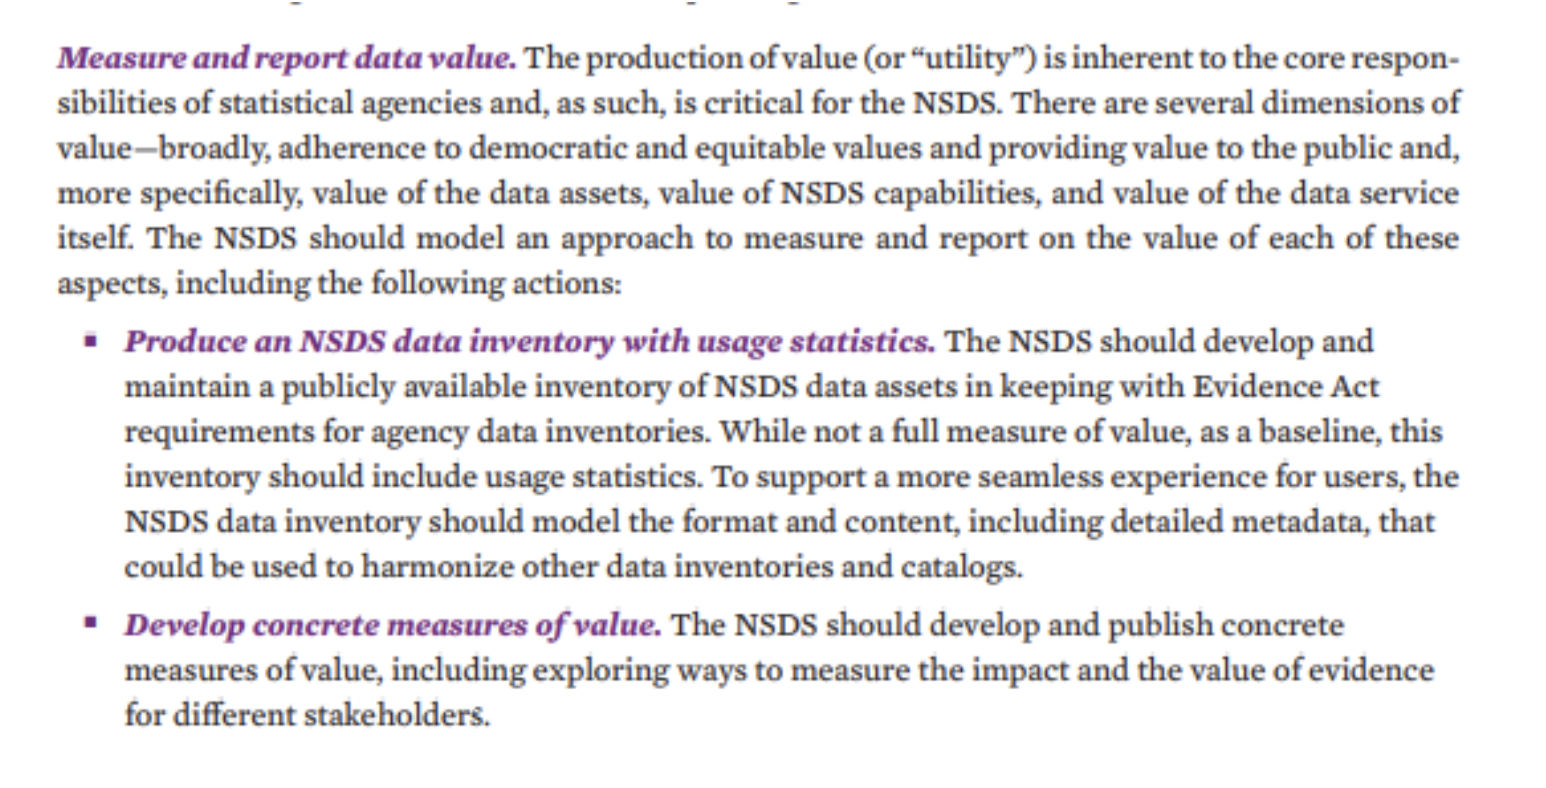
\includegraphics[scale=0.50]{Advisory.png}
  \caption{Recommendation of ACDEB}
  \label{fig:advisory}
\end{figure}

The platform can also support the Standard Application Process by providing information to researchers about the use of federal data assets in the Federal Statistical Research Data Center system. 

\subsection {History}
The project began in 2016 when NYU was asked by the US Census Bureau to build a secure environment to host confidential microdata to inform the decision making of the Commission on Evidence-Based Policymaking. It quickly became apparent that simply hosting data was insufficient; a search and discovery functionality was needed to find out 
\begin{enumerate}[label=(\roman*)]
\item \textbf{how} data are used, so that government agencies can better understand the utilization of their data investment portfolio and scientists can find other ways in which data have been used 

\item by \textbf{whom}, so that government agencies and their stakeholders as well as scientists (particularly junior faculty and graduate students) can find experts,

and

\item to study what \textbf{topics} so that government agencies can identify how well their data investments are supporting their mission and scientists can find other work that is complementary to their own.
\end{enumerate}


The challenge was that the information about data use is not readily found - A joint project between the developers of Jupyter - Brian Granger and Fernando Perez - and Julia Lane of NYU was funded by the Alfred P. Sloan Foundation and Schmidt Futures to see if it was possible to use Machine Learning and Natural Language Processing tools to automate the discovery of dataset mentions in scientific documents.  The team developed and hosted the first \href{https://coleridgeinitiative.org/richcontextcompetition}{rich context competition} in 2018; the results were reported in a Sage \href{https://study.sagepub.com/richcontext}{book} published in 2019\cite{source1}. 

A national \href{https://coleridgeinitiative.org/richcontext/richcontextworkshop/}{conference} was subsequently hosted at the National Press Club in November 2019 – also funded by Schmidt Futures and the Alfred P. Sloan Foundation - which was designed to produce a \href{https://coleridgeinitiative.org/wp-content/uploads/2022/01/WorkshopReport_November-25_final_Jan-6_2020.pdf}{roadmap} to identify the opportunities, gaps, and necessary investments, develop an interdisciplinary community of computer scientists, life scientists, and social scientists who can work together to address the problems and engage key stakeholders, notably funding agencies, and government agencies.


The output from the workshop fed into continuing work and during 2021,  the effort resulted in a \href{https://www.kaggle.com/c/coleridgeinitiative-show-us-the-data}{Kaggle competition}, known as Show US the Data to develop open algorithms that would improve on the previous efforts. Over 1600 data science teams worldwide competed. The winning algorithms were unveiled at a \href{https://www.youtube.com/watch?v=H3uOkBzsAFg}{conference} in October 2021 hosted by the Coleridge Initiative and the open access consortium \href{https://www.chorusaccess.org/}{CHORUS} and they are the ones currently used in the platform.


A pilot was then initiated with one of the CHORUS board members, Elsevier, to test the possibility of connecting agency datasets with a fully curated corpus of publications, Scopus (\hyperref[fig:links]{Figure 2}), and policy documents (\hyperref[fig:policy_impact]{Figure 3}).

\begin{figure}
  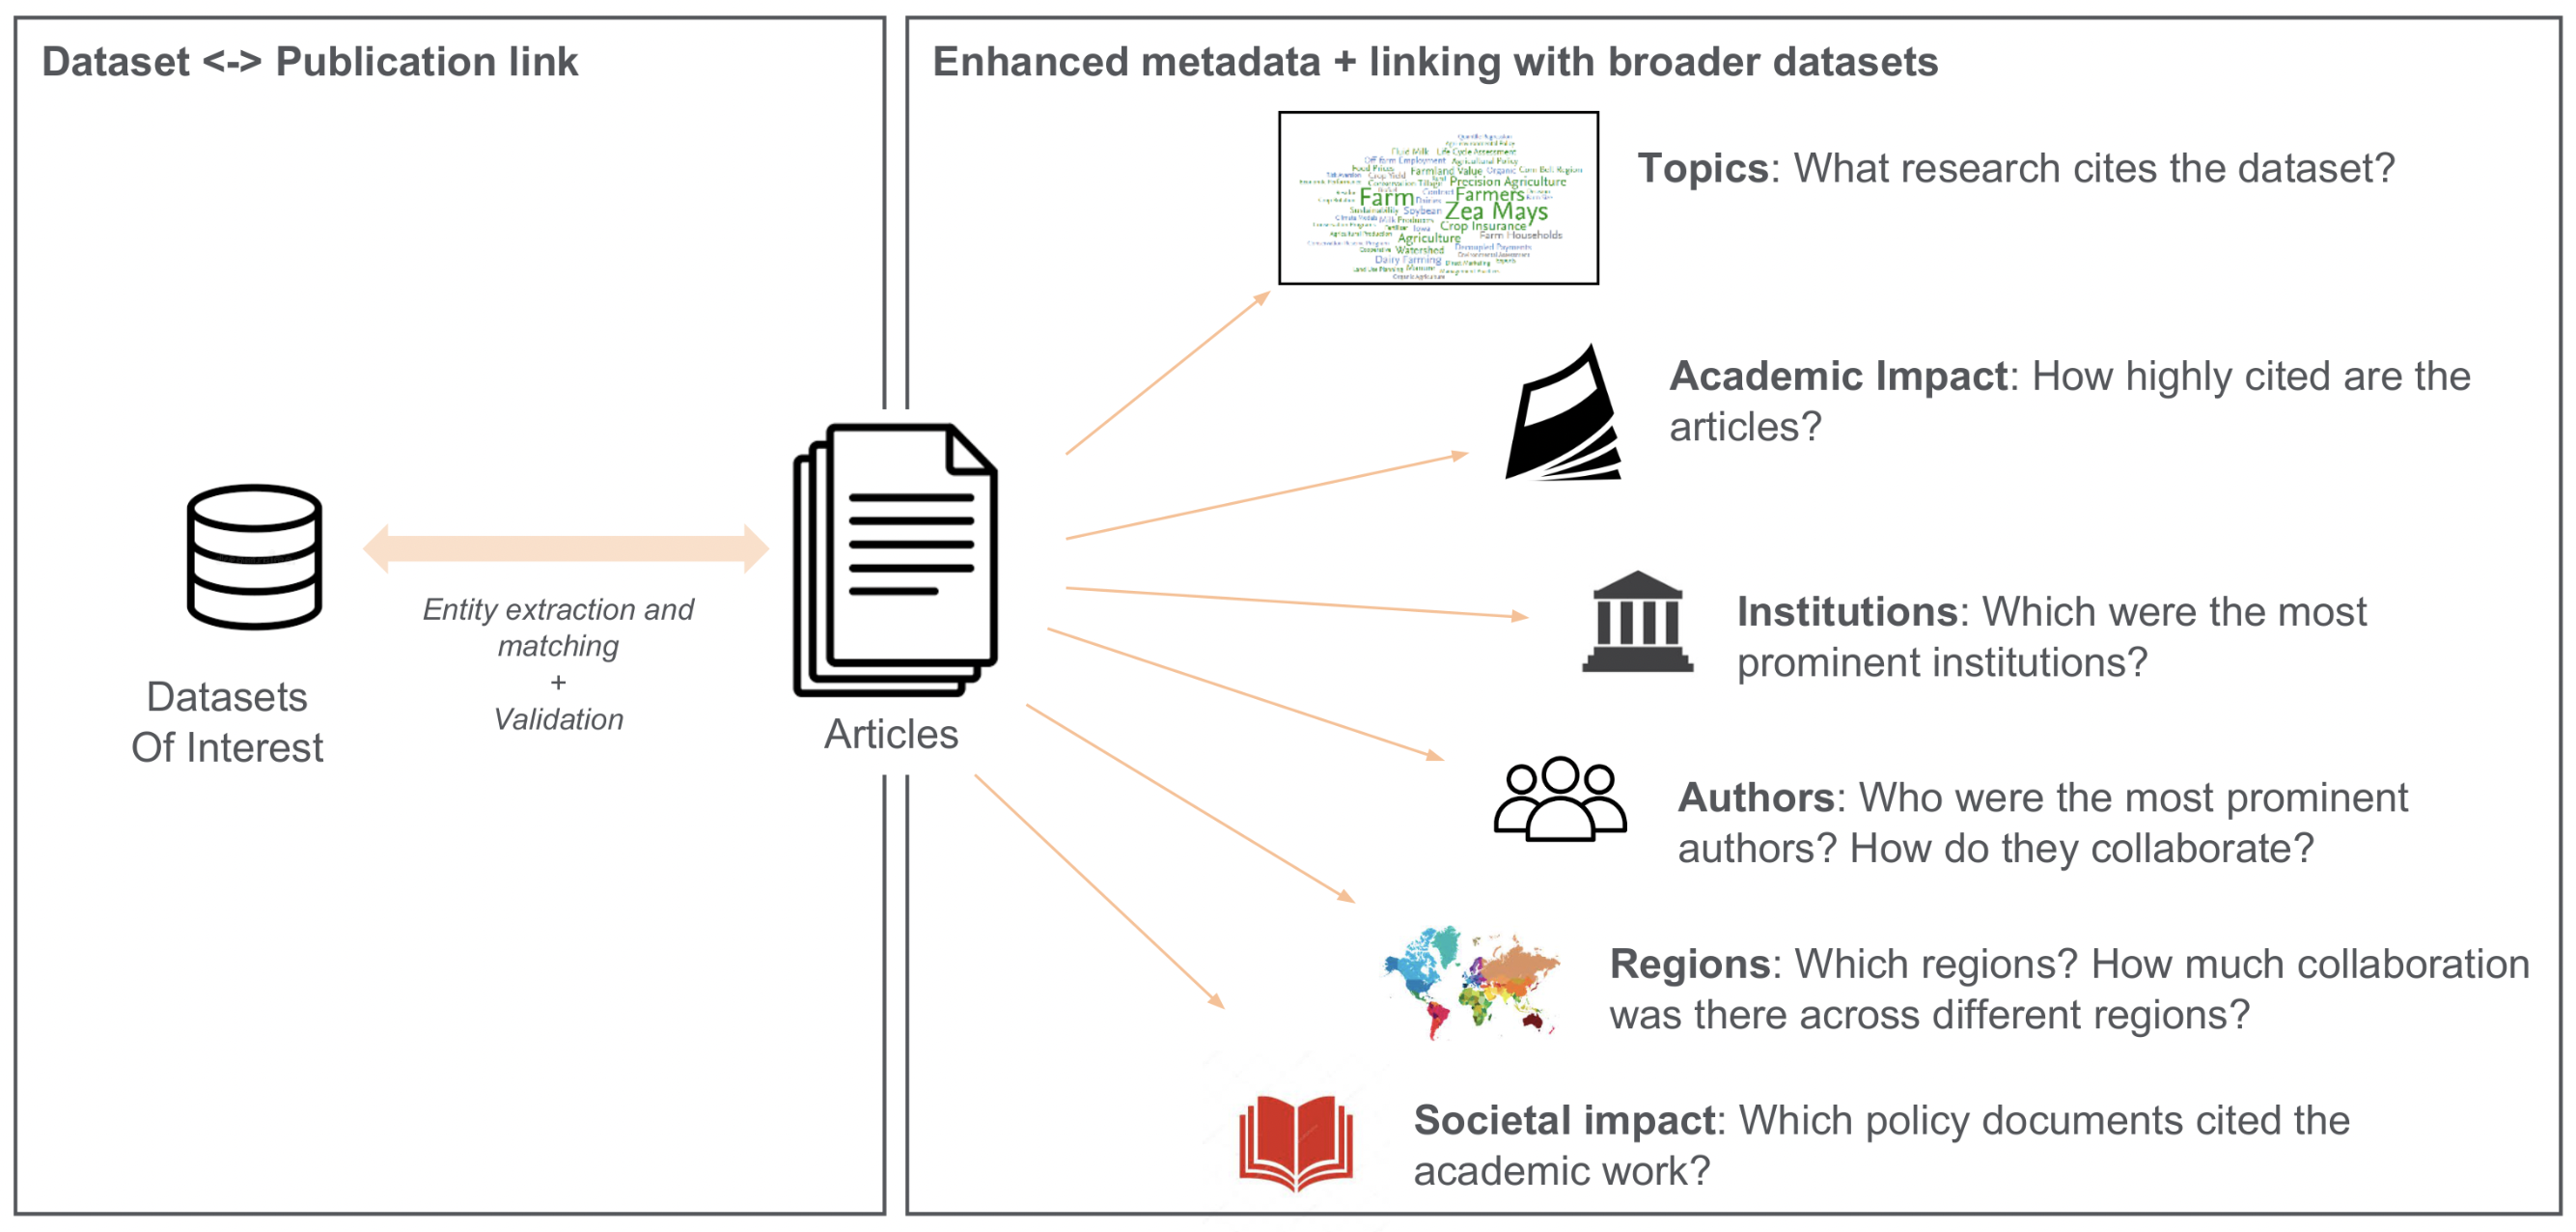
\includegraphics[scale=0.35]{links_dataset_publication.png}
  \caption{The links between agency datasets and publications}
  \label{fig:links}
\end{figure}

\begin{figure}
  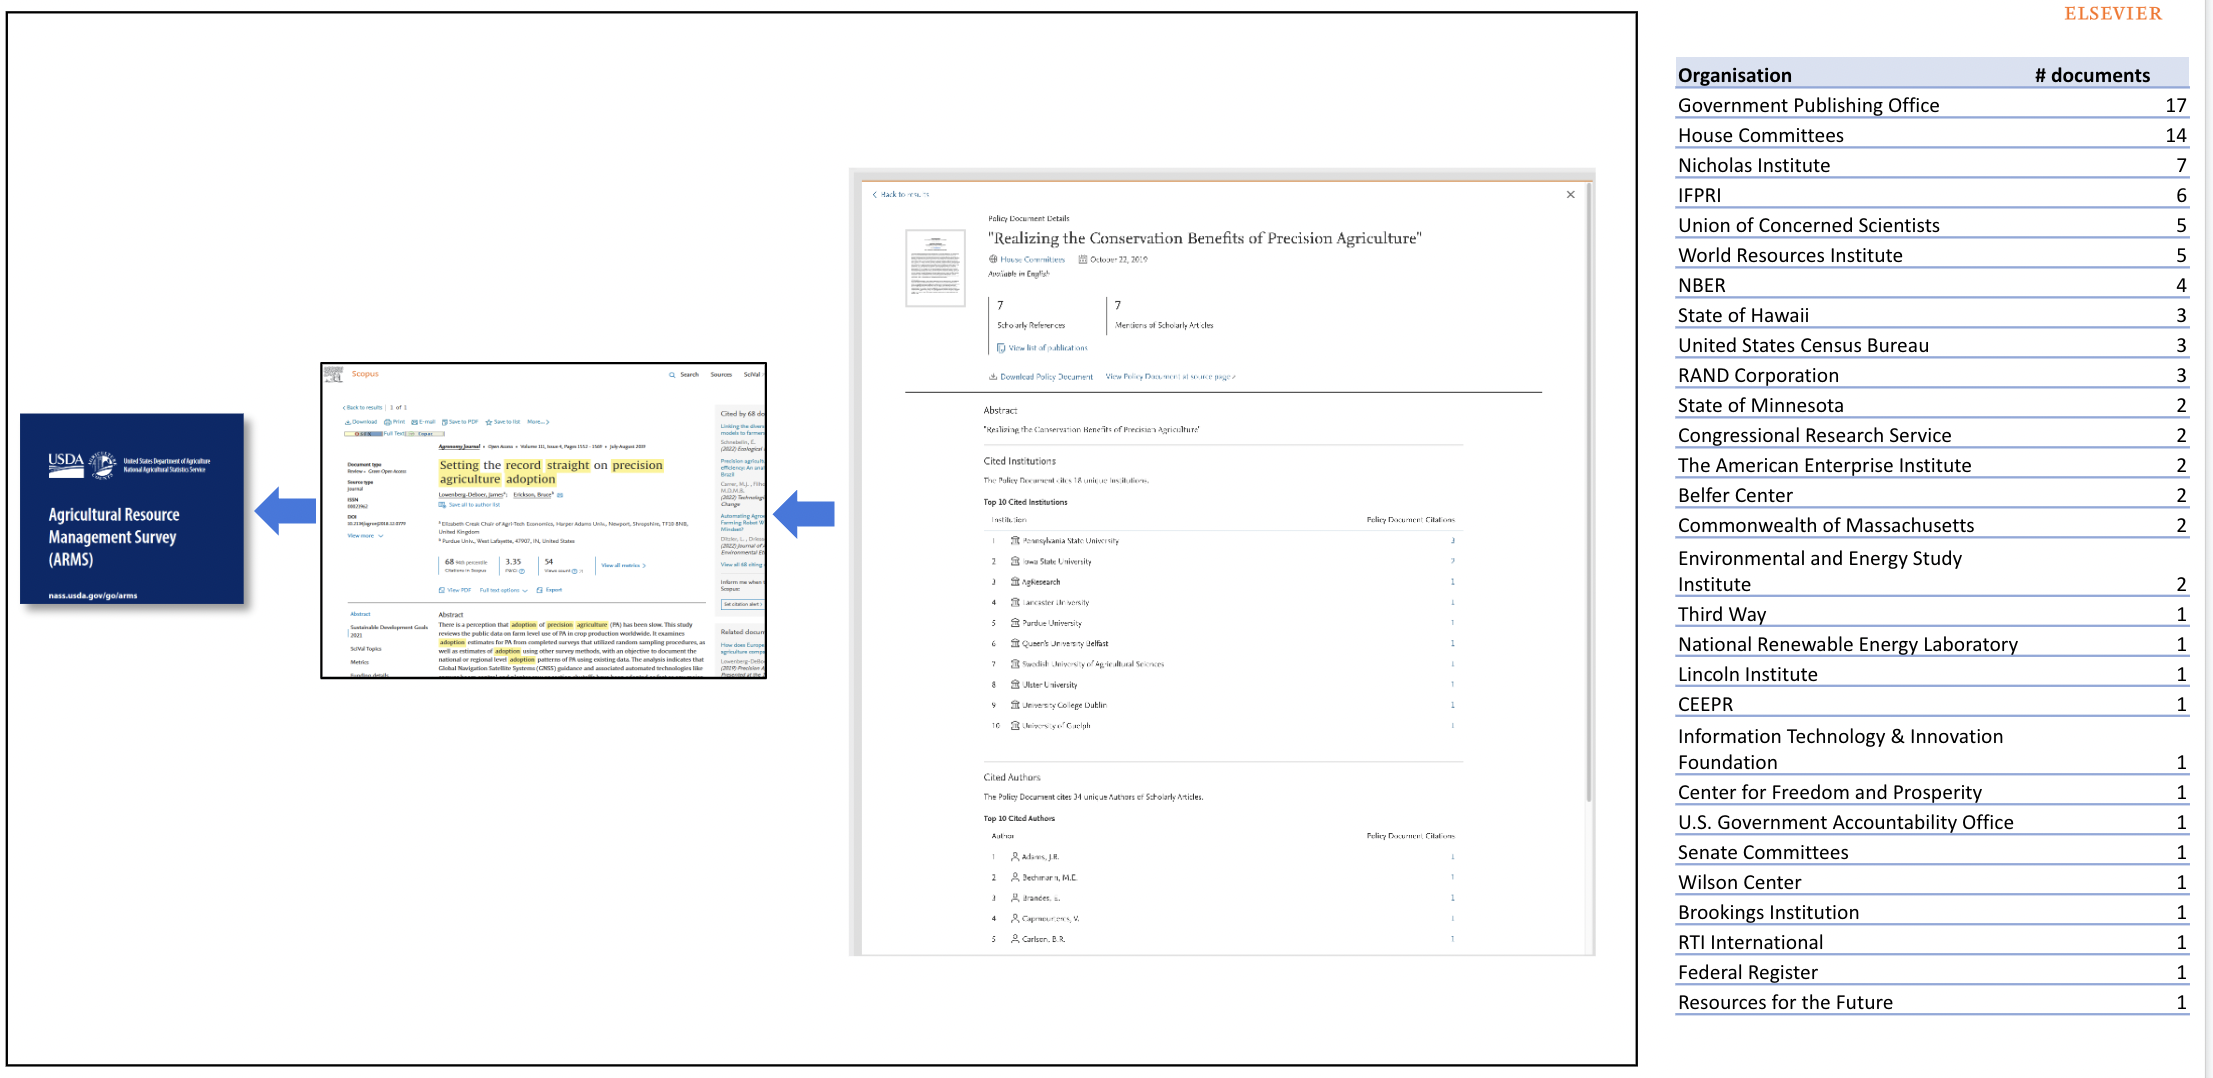
\includegraphics[scale=0.42]{policy_impact.png}
  \caption{The potential next links to policy impact}
  \label{fig:policy_impact}
\end{figure}

\subsection{Academic and Research Partners}
The project is the result of a collaboration among six academic partners.   The role of each is described below.

\underline{\textbf{NYU}}: New York University (NYU) is responsible for overall coordination and management of the effort to develop and implement the platform. The NYU team is the primary agency contact.

\underline{\textbf{Elsevier}}: Elsevier provides the information infrastructure - the curated corpus of documents such as publications and patents - that provides the basis on which to run the algorithm, optimizes the search space, applies the existing algorithms to search and discover specific datasets, and produces metadata to feed into the validation process and the API, dashboards, and Jupyter Notebooks.

\underline{\textbf{The Institute for Data Intensive Engineering and Science (IDIES) at Johns Hopkins}} \\ \underline{\textbf{University (JHU)}}: IDIES ingests and processes the metadata output from the ML algorithm into a database that can be validated in the validation tool. then feeds the validated output to the API. IDIES developed the validation tool so that the agencies or their designated collaborators can validate the output. IDIES also developed \href{http://www.sciserver.org/}{SciServer}, a collaborative, web-based science platform. 

\underline{\textbf{Texas Advanced Computing Center (TACC)}}: Designed, developed, and is implementing the API to disseminate the validated metadata received from JHU. TACC also has enabled the front-end tool implementation by enabling the web connector for Tableau software for visualization in a dashboard. TACC will be developing a browser-based dashboard.

\underline{\textbf{University of Texas at San Antonio (UTSA)}} is validating the ML output for some agencies.  They will also work to support ML model development and the researcher engagement at conferences. Their team will play an important role in analyzing and promoting the progress and success of the project.

\underline{\textbf{University of Maryland, College Park (UMD)}} is developing a website that describes the methodology, approach, and relevant materials for the user community.  They will jointly host one or more workshops for researchers to react to the findings and measurement.

\subsection{Current Agency Partners}
\underline{\textbf{National Center for Science and Engineering Statistics (NCSES)}}: NCSES supported the work \\from the earliest stages. Their goal was to show how NCSES data were being used and tie the information into their revamped website.   Later, the development of usage statistics is likely to be important as they establish the National Secure Data Service.

\underline{\textbf{US Department of Agriculture}}: Economic Research Service (ERS) also supported the work from the earliest stages. It set the initial direction of tool development and implementation.  The National Agricultural Statistical Service (NASS) worked with ERS to identify the initial USDA data sets and possible visualization tools, identified validators (either internal or external). They also will conduct research to develop a theory of change and will develop targeted messages to survey respondents to increase overall response rates.

\underline{\textbf{Department of Education}}: National Center for Education Statics (NCES) has a number of goals: 
\begin{description}[labelindent=1cm] 
\item [Relevancy] Determine who is using NCES data, including networks of dominant users; 
\item [Priority] Understand which data sets are being used the most and which the least; 
\item [Equity] Gain an equity perspective on use of NCES data; 
\item [Community] Build partnerships with researchers who are conducting research in areas of interest to NCES. 
\end{description}

\underline{\textbf{Department of Commerce}}: The National Oceanic and Atmospheric Administration (NOAA)’s primary objective was to develop a reusable data discovery interface. The overall goal for NOAA is to use machine learning to find citations to NOAA datasets in journal articles and other scientific literature. This knowledge will help highlight the value of NOAA’s open data, track the provenance of data used in scientific research, and help new users find trusted data that is relevant to their research topic.

\underline{\textbf{National Institutes of Health}}: The primary objective is to provide a rich and innovative set of tools for addressing data sharing problems by enabling search and discovery for the subsequent use of NIH funded digital data assets. The NIH project is sponsored by the Office of Data Science Strategy.  It will identify a subset of HIV datasets found in Mendeley Data\footnote{\url{https://data.mendeley.com}} and find the publications that cite those datasets.  It will expand information the use of data in the Mendeley data repository, such as number of views and downloads to include other aggregate measures generated from the Democratizing Data platform such as diversity of use, use within specific disease ecosystems and ecosystem services, use within particular communities, and use of particular historical significance\cite{source2} . The team will also develop dataset use at the researcher level, to identify and encourage experts who share their expertise, as well as at the institutional level to help inform program investment decisions. The platform will enable NIH/ODSS to extend to and engage with their associated communities, following on from the January 2022 \href{https://datascience.nih.gov/data-infrastructure/search-workshop}{ODSS dataset search workshop}\cite{source2}.  

\section{WORKFLOW OVERVIEW}
\label{sec:Chapter3}
There are three main workflow stages: identifying and finding datasets in publications (process); providing agency and researcher access to information through APIs, Jupyter Notebooks and usage dashboard (access and disseminate), and getting feedback from the user community (feedback).

\subsection{Process}

\begin{figure}
  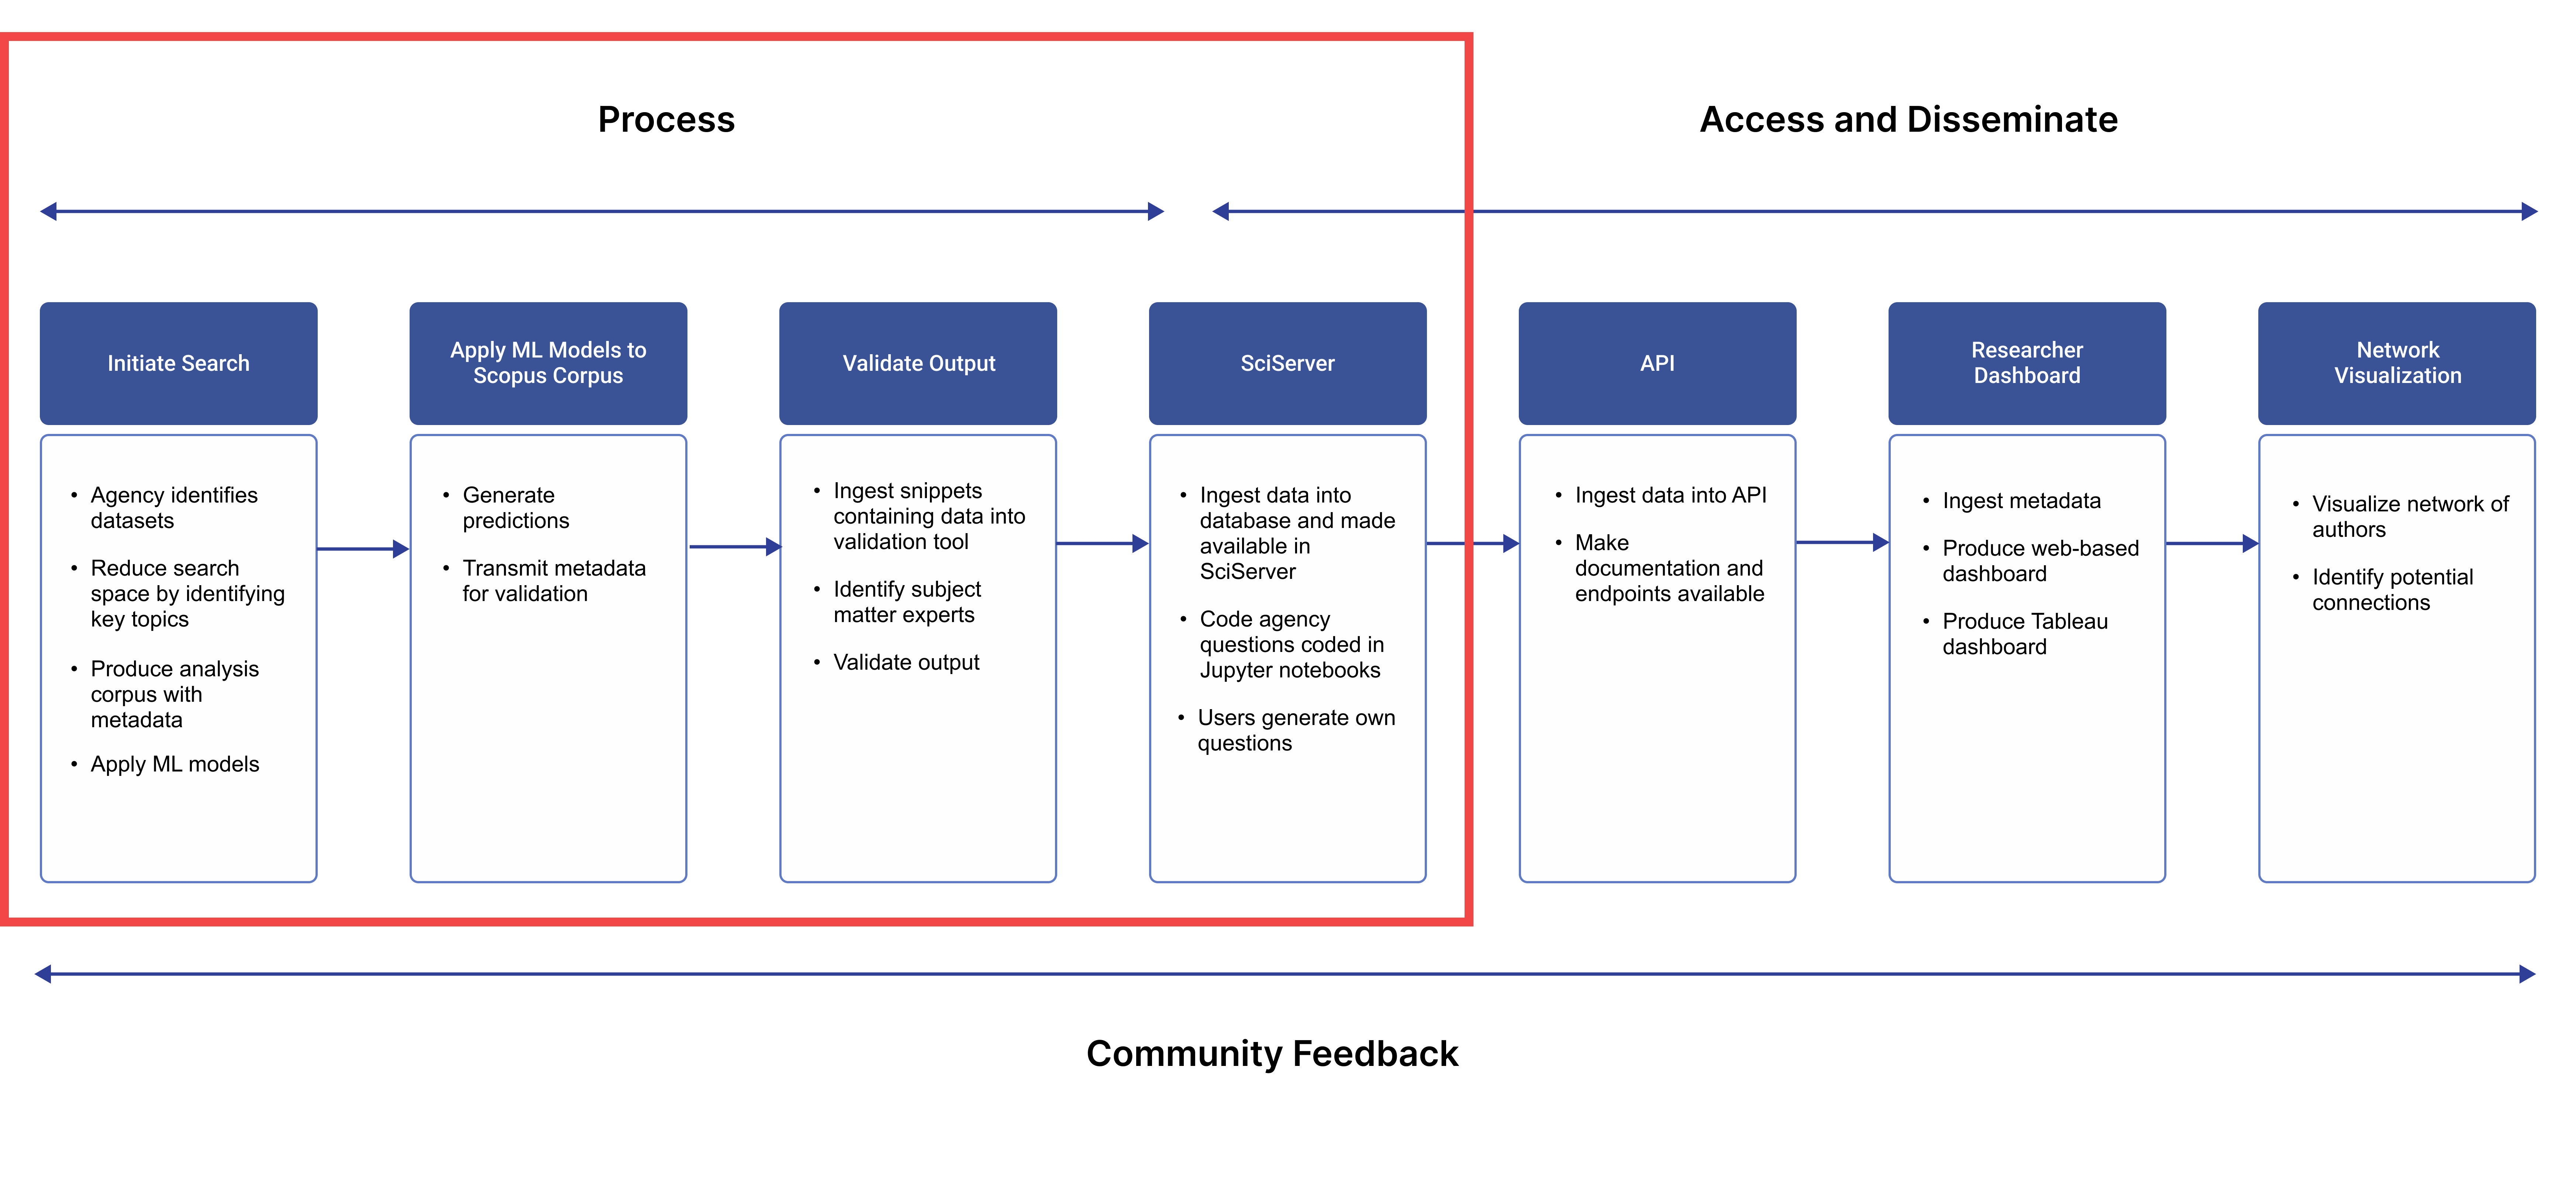
\includegraphics[scale=0.20]{Process.png}
  \vspace{-2.5ex}
  \caption{Process}
    \vspace{-0.97ex}
  \label{fig:process}
\end{figure}

\begin{description}
\item [Initiate search:] An agency identifies a list of datasets of interest (target datasets), ideally including commonly used dataset aliases and, where available, the dataset digital object identifier (DOIs).  Elsevier works with NYU to identify a search corpus of full text publications on which the ML models can be run.  For more details see \hyperref[sec:Chapter5]{Chapter 5}.


\item [Apply ML models:] Elsevier runs the three ML models to identify candidate datasets mentioned in publications within the search corpus, producing as output:\begin{enumerate*}
    \item the dataset-publication pairs (dyads)
    \item snippets of text containing the mention to assist in validation and
    \item associated metadata on ML performance and other relevant runtime parameters.
\end{enumerate*} Machine Learning algorithms are applied to the licensed full text records in the search corpus to identify those research outputs which contain candidate datasets. The ML algorithms are then further supplemented with matching routines that search for closely related strings (fuzzy matches). The final step in the Elsevier workflow is to generate the metadata for the research outputs identified as containing the datasets. For more details, see \hyperref[sec:Chapter6]{Chapter 6}. 

\item [Validate:] The output of those models predicts whether a dataset is mentioned, and Elsevier provides the metadata (journals, authors, institutions, geographic locations and research topics inter alia) associated with those publications to IDIES at JHU for validation. 

\end{description}
IDIES retrieves the output information from Elsevier via a predefined secure transport mechanism (in this case delivery of data to an AWS S3 bucket). It then performs a set of automated validations of the format and consistency prior to loading from the file-based format to a relational database. In this process files are cached within the SciServer (described below) environment for further inspection as necessary.

The metadata are ingested into a database (schema is available in \hyperref[sec:APPENDIXA]{Appendix A}; the metadata table and data dictionary in \hyperref[sec:APPENDIXB]{Appendix B}) and made available to designated agency staff to validate the output in a validation tool.  They validate the data by inspecting snippets and validating the ML identification via a web-based tool.  This is a first pass in the quality control of the output metadata. There is the potential of adding additional features if resources are available. In particular, researchers could provide additional validation of the results of the ML algorithm by providing feedback on publications that may have been missed or mischaracterized, since the validation process creates rich opportunities for participation and engagement. For more details, see \hyperref[sec:Chapter7]{Chapter 7}.

Once complete, the full result, including validation is sent to TACC to be ingested in the official API for consumption by end-users.

An administrative dashboard is also being built; that documentation will be made available in Version 2 of this user guide.

The full technical description of this workflow is available in \hyperref[sec:APPENDIXC]{Appendix C}.

\subsection{Access and Dissemination}
There are three access modalities: Jupyter Notebooks, an Application Programming Interface (API), and an interactive usage dashboard.  Each is designed to provide different insights into answering the core \hyperref[subsec:Agencyquestions]{Agency Questions} that are the reason for building the Search and Discovery Platform.

% TODO: insert figure
\begin{figure}
  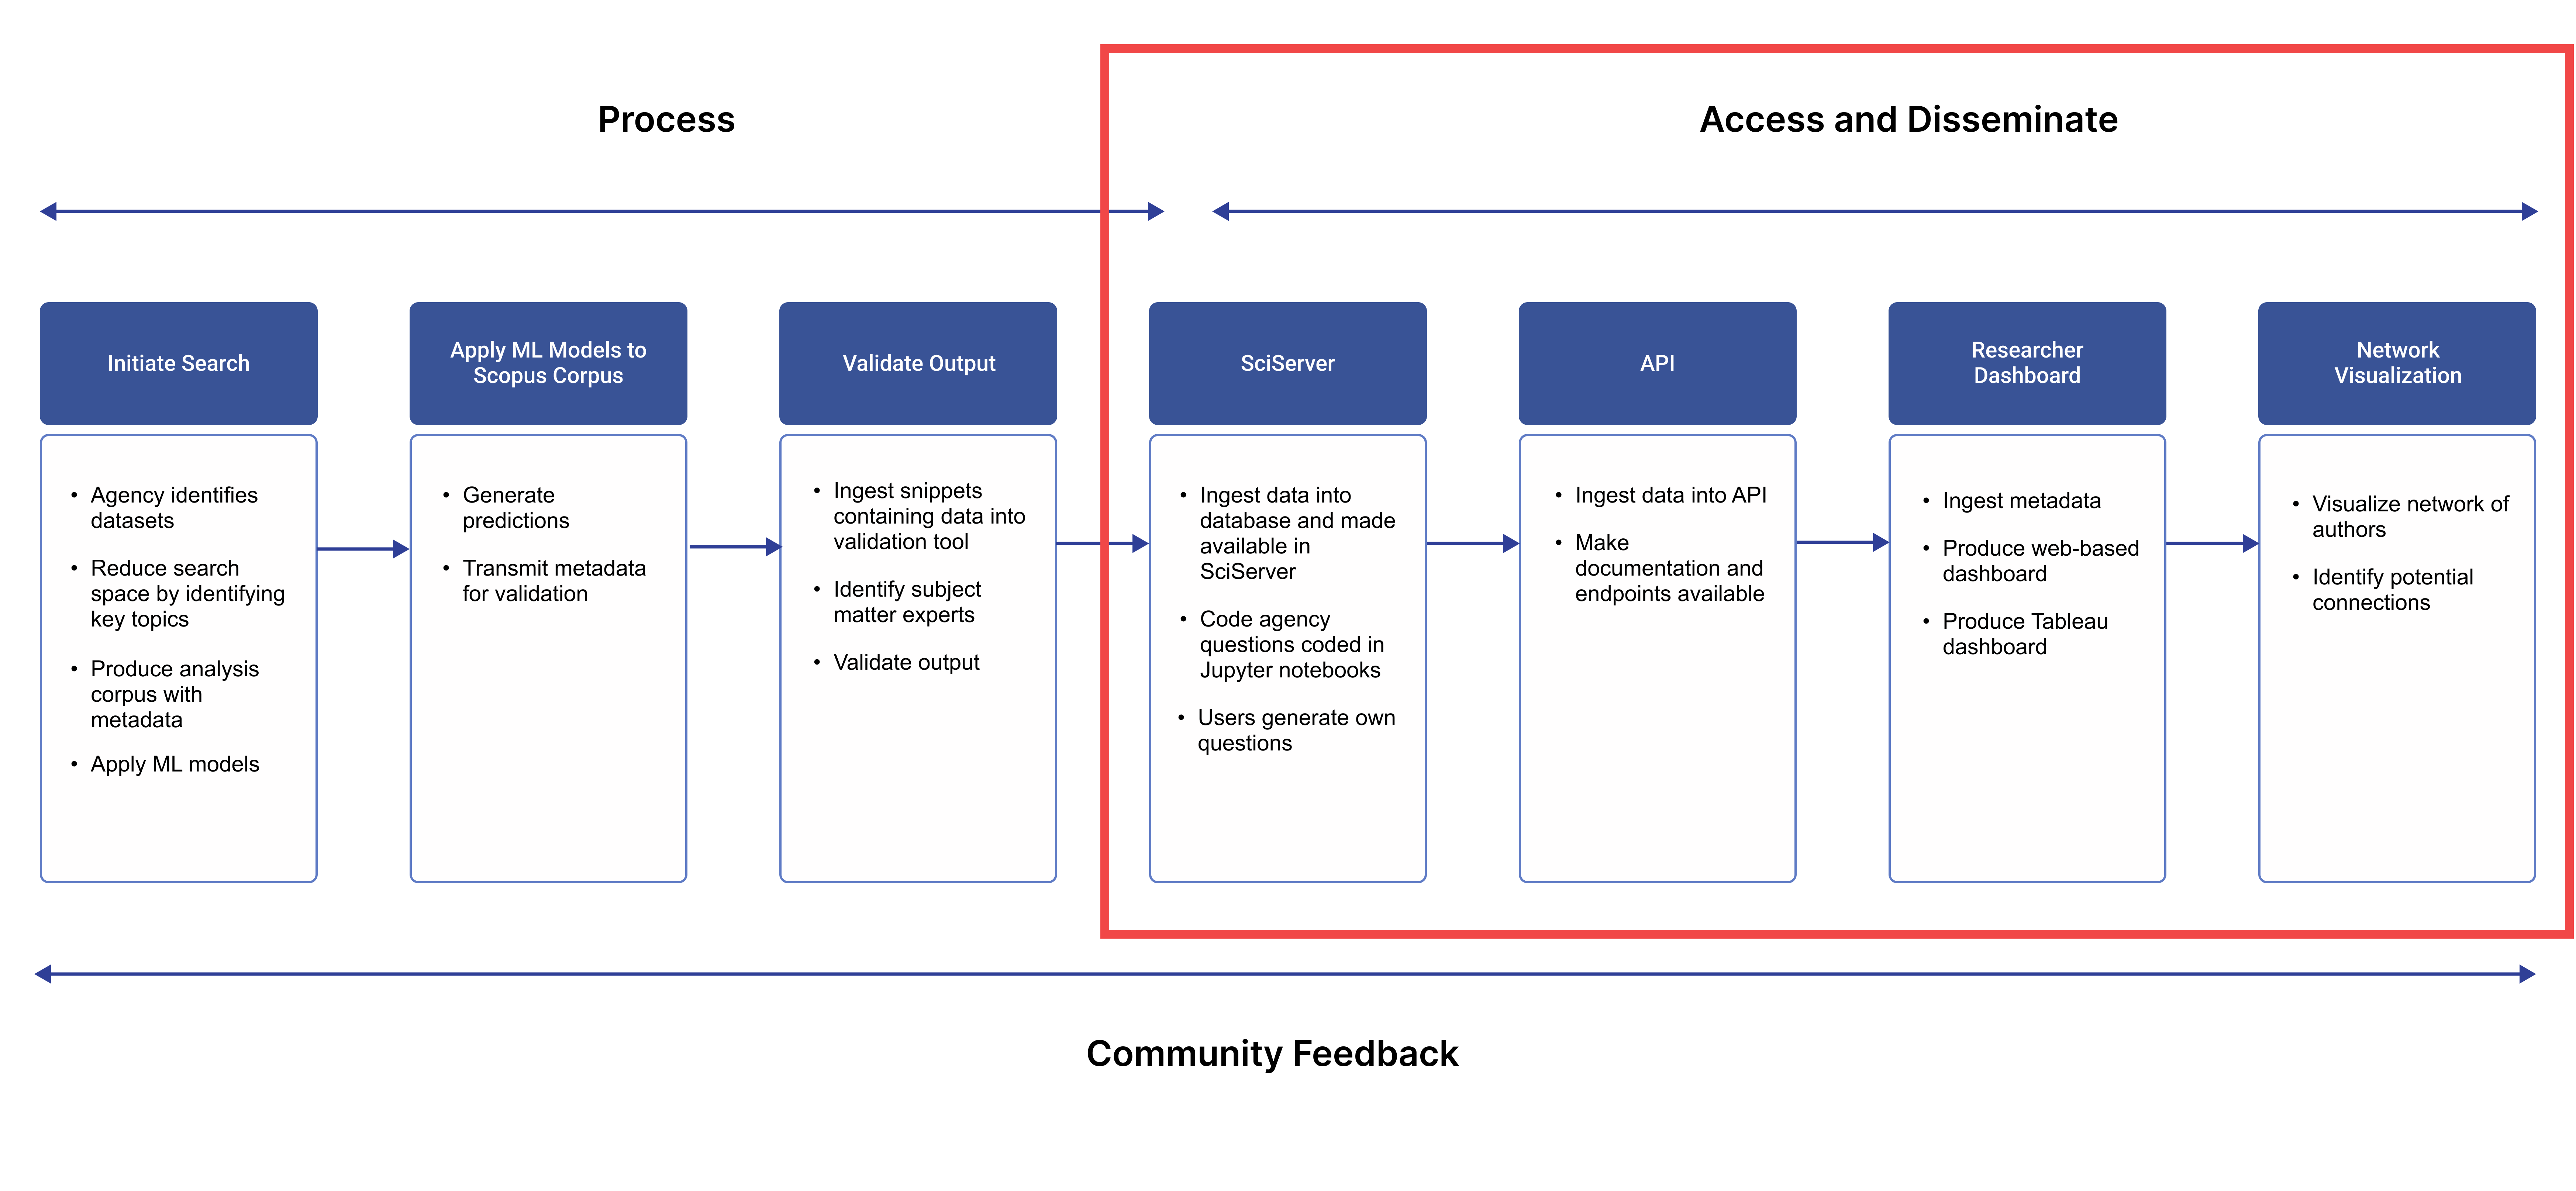
\includegraphics[scale=0.20]{Access.png}
  \vspace{-2.5ex}
  \caption{Access and Disseminattion}
    \vspace{-0.97ex}
  \label{fig:access}
\end{figure}

\begin{description}
\item [Jupyter Notebooks:] The Jupyter Notebooks can be accessed through SciServer \url{https://www.sciserver.org}, which is a science platform built and supported by the Institute for Data Intensive Engineering and Science (IDIES).  Sciserver builds upon and extends the SkyServer system of server-side tools that introduced the astronomical community to SQL (Structured Query Language) and has been providing the Sloan Digital Sky Survey catalog data to the public. 

The Jupyter Notebooks are structured to enable researchers to access a database that contains the metadata. Researchers can either program their own queries or access a preprogrammed set of 20 questions about use of the data. SciServer allows researchers to collaborate using hosted data sets in a secure environment, among many other features. For more details, see \hyperref[sec:Chapter8]{Chapter 8}.

\item [Application Programming Interface (API):] The API allows users to download the metadata in order to create their own dashboards or methods of analysis. The endpoints reflect the key information requested by the agencies - publications, citations, authors, institutions, locations, and journals.  The API has a web data connector that allows the metadata to be downloaded into Tableau software to create visualizations. For more details, see \hyperref[sec:Chapter9]{Chapter 9}.

\item [Dashboard:] The dashboard and other visualizations illustrate:\begin{enumerate*}[label=(\arabic*)]
    \item how data are being used for research;
    \item the primary topics of the research;
    \item the researchers who have published;
    \item how often that research has been cited; and 
    \item institutions affiliated with the researchers.
\end{enumerate*} The dashboards can be structured to inform the agency that is producing the data or also to be a community dashboard that is accessed by the research community and greater public. The dashboard is a type of researcher “leaderboard”, identifying the top researchers for different datasets based on the number of their publications and citations. This enables an understanding of who is using the data and their topics of study and helps build collaborative communities. The ancillary benefit to the researchers is a place where their publications can be widely seen and cited in future research, thus encouraging other agencies and collaborators to join in.
\end{description}

In addition, the project team created a sample of five-minute podcasts with top researchers to discover more about their research and how it benefits the public.  The researchers were able to provide advice to other researchers using or considering using the data sets, as well as suggestions for how agencies could improve their data and make it more useful.  The sample podcasts were published in the Harvard Data Science Review and are available \href{https://hdsr.mitpress.mit.edu/pub/gnf4pmig/release/3}{here}. As participation increases, these podcasts can be embedded in the API or dashboard, providing practical advice to researchers considering using the identified data sets.  For more details, see \hyperref[sec:Chapter9]{Chapter 9}.

\section{CORPUS DEVELOPMENT}
\label{sec:Chapter4}
\subsection{Source Data}
The data that Elsevier searches as part of its contribution to Democratizing Data is drawn from Scopus. Scopus is the largest abstract and citation database of peer-reviewed literature: scientific journals, books and conference proceedings. As at May 2022, Scopus contained 87 million records, from over 7,000 publishers over 100 countries. Around 11,000 new records are indexed every day\cite{source3,source4,source5} . 

Elsevier is itself a significant publisher of research. During 2019, Elsevier accounted for the review, editing and dissemination of 18\% of the world's scientific articles. Scopus draws on this rich publishing heritage but also benefits from relationships with other publishers, most of whom have provided licenses that enable Elsevier to search the full text in order to identify key metadata or data elements. Nevertheless, there are some exceptions. For example, for the Democratizing Data project Elsevier is not licensed to undertake full text searchers from Springer Nature so their records must be excluded from the search routines.

\subsection{Seed Corpus}
The standard corpus creation process used by Elsevier starts with the creation of a seed corpus based upon the target datasets and aliases (or alternative names) for each dataset. In addition, some agencies are able to provide either references to a sample of actual articles in which the datasets have been used or to the names of candidate journals in which articles are likely to be found.

Having high quality information from the relevant agency helps to ensure that the search space is more targeted to the likely publications; this helps improve precision and recall, in particular ensuring that false positives are minimized.  The target dataset names and aliases are recorded and form part of the job run metadata.

The seed corpus is created using exact string matching of the target datasets and aliases against Elsevier’s Science Direct database. This database contains research outputs published by Elsevier (over 2,500 journal and 40,000 book titles). The Wikipedia entry for Science Direct can be found \href{https://en.wikipedia.org/wiki/ScienceDirect}{here}. 

From the matched publications, Elsevier identifies a set of research Topics.  A \textbf{Topic is a collection of publications with a common intellectual interest} and can be large or small, new or old, growing or declining. A Topic is defined to be where the direct citation linkages within the Topic are strong and the direct citation linkages outside the Topic are weak. Only the indexed publications are included in Topics. There are 96,000 Topics and these are grouped into 1,500 Topic Clusters. Over time, new Topics will surface, and as Topics are dynamic, they will evolve. For the search corpus creation, the Elsevier team employed the more detailed Topics. A publication can belong to only one Topic and a Topic can belong to one Topic Cluster. More on Topics can be found in the footnote below\footnote{\url{https://www.elsevier.com/solutions/scival/features/topic-prominence-in-science}\\\url{https://www.elsevier.com/__data/assets/pdf_file/0006/548313/Topic-Prominence-Advanced-Webinar.pdf}}. 

The Topics, together with any other parameters (e.g., date range) specified by the agency, are then used to identify the corpus of full text articles that form the basis of the Search Corpus. At this point, the publishers of the full text articles are checked and those records are excluded from the corpus where the license agreement does not allow for Elsevier to undertake full text analysis.

\subsection{Coverage of Full Text Research Outputs}
The following table provides a summary of full text records that are available and searchable based on the calendar year of publication during the period 2017 to 2021. Full text records are, of course, also available for earlier periods although as one goes further back in time, the number of full text records decreases. This table is designed to illustrate the possibilities in the search space for what we have found to be typical periods of interest. 

\vspace{0.5cm}

\begin{table}[h!]

{\renewcommand{\arraystretch}{1.5}%
\begin{tabularx}{1\textwidth} { 
  | >{\raggedright\arraybackslash}X 
  | >{\raggedright\arraybackslash}X 
  | >{\raggedright\arraybackslash}X 
  | >{\raggedright\arraybackslash}X
  | >{\raggedright\arraybackslash}X
  | >{\raggedright\arraybackslash}X 
  | >{\raggedright\arraybackslash}X |}
 \hline
 {\bf Calendar Year} & {\bf Scopus Records} & {\bf Records with Full text} & {\bf Elsevier’s own Full Text  Records} & {\bf Full Text Records Licensed and available for Search} & {\bf Licensed as \% of Full Text Records} & {\bf Licensed as \% of Scopus Records} \\
 \hline
 {\bf 2021 }& 4,079,818 & 3,826,784 & 701,724 & 3,428,470 & 89.59\% & 84.03\% \\
 \hline
 {\bf 2020 }& 3,856,004 & 3,583,017 & 645,188 & 3,233,503 & 90.25\% & 83.86\% \\
 \hline
 {\bf 2019 }& 3,644,970 & 3,392,420 & 597,381 & 3,091,172 & 91.12\% & 84.81\% \\
 \hline
 {\bf 2018 }& 3,455,000 & 3,152,839 & 576,948 & 2,881,415 & 91.39\% & 83.40\% \\
 \hline
 {\bf 2017} & 3,270,051 & 2,843,709 & 553,854 & 2,594,161 & 91.22\% & 79.33\% \\
 \hline

\end{tabularx}
\caption{Full text records available and searchable based
on the calendar year of publication during the period 2017 to 2021.}
\label{table:1}
}
\end{table}

\vspace{0.5cm}

As more fully described in the next chapter, the Machine Learning algorithms are applied to the licensed full text records in the corpus to identify those research outputs which contain candidate datasets. The ML algorithms are then further supplemented with fuzzy matching routines. The final step in the Elsevier workflow is to generate the metadata for the research outputs identified as containing the datasets. 

\section{THE ML ALGORITHMS}
\label{sec:Chapter5}

To support the identification of datasets within a set of full text publications, the community was engaged through a Kaggle competition \url{https://www.kaggle.com/competitions} in 2021 to develop and identify the best Machine Learning (ML) and Natural Language Processing (NLP) tools. About 1,600 data science teams entered, and seven winners were identified and provided their data, code and methodology as open-source tools for public use\cite{source2,kaggle,ghani,source7} . Of these seven, Elsevier uses the top three to identify datasets within the full text of the search corpus. 

\subsection{The Kaggle Models}
\begin{description}[style=nextline]
\item [Model 1 (Deep Learning - Sentence Context)]
This model’s approach is to use a deep learning-based approach to learn what kind of sentences have references to a dataset. This model takes the longest to run, but also is the most robust to new datasets. It evaluates all of the text within the document.

\item [Model 2 (Deep Learning - Entity names)]
This model’s approach extracts names of entities from the text and uses a deep learning-based approach to classify an entity as being a dataset or not. This model runs faster than model 1, but is slightly less robust to new datasets.

\item [Model 3 (Pattern Marching)]
This model takes a rule-based approach to search for patterns in the document that are similar to a list of existing datasets. This is the fastest model to run, but is the least robust.

\end{description}

During the Kaggle competition, it was determined that the ML models were able to pick up a wider variety of ways in which authors refer to the same datasets than was possible through simple string searches. This was especially true for the winning model “Context Similarity via Deep Metric Learning” which learnt from the context and did not just rely on the way in which the aliases were written in the training set. 

In terms of the computer processing, it is simpler and faster to run approaches not relying on Deep Learning methods: Models 2 and 3 performed well if applied to publication domains like the one used on the Kaggle competition. The competition also demonstrated that there was little overlap in the datasets identified by the different models. 

\begin{table}[h!]

{\renewcommand{\arraystretch}{1.5}%
\begin{tabularx}{1\textwidth} { 
  | >{\raggedright\arraybackslash}X
  | >{\raggedright\arraybackslash}X 
  |}
 \hline
 {\bf Model Name} &{\bf Methods Used}  \\
 \hline
 Context Similarity via Deep Metric Learning & Searching candidates in certain format + Filtering out prediction based on keywords + Searching based on the frequency of dataset appearance + Masked language model  \\
 \hline
 Transformer-enhanced Heuristic Search & Searching candidates in certain format + Searching based on the frequency of dataset appearance + Models learning from candidate strings  \\
 \hline
  Simple and Strong Baseline & Searching candidates in certain format + Filtering out prediction based on keywords + Searching based on the frequency of dataset appearance  \\
 \hline
 
\end{tabularx}
\caption{Top ML Models From Kaggle Competition: Models and Methods.}
\label{table:1}
}
\end{table}

\subsection{The Application of the Models}
Building on the outcomes and findings of the Kaggle competition, in undertaking the full text search, Elsevier employs all three of the winning Kaggle models. In addition to the identified dataset, each model generates a score that reflects the certainty of the model about the identified mention. The generation of the score is built into each Kaggle algorithm. Elsevier does not apply any thresholds with regard to the Kaggle scores, but rather ingests the full output of datasets generated from the algorithms.

The text identified by the models as being a potential dataset as well as their scores are extracted and stored. In addition, at this point and where licenses allow, a data snippet is generated from the full text showing the text [235 characters] immediately before the candidate dataset text string and the text [235 characters] immediately after the candidate dataset text string. This snippet is used in the validation process i.e. used to identify whether a match is a true match or a false positive.

There is a range of logical possibilities for each full text publication record searched:

\begin{itemize}
    \item No dataset found in the publication;
    \item Single dataset found (extracted and single output record produced). This record may or may not be from a target dataset (target dataset in this respect being a dataset provided by the agency or one of its aliases);
    \item Multiple references to a single dataset found (extracted and multiple output records produced). This record may or may not be from a target dataset(s);
    \item Single reference to multiple datasets found (extracted and multiple output records produced). This record may or may not be from a target dataset(s);
    \item Multiple references to multiple datasets found (extracted and multiple records produced). (Again, these may or may not be to target dataset).
\end{itemize}

\subsection{Finding Target Datasets}

At this point, the Kaggle algorithms have been applied to the full text and have identified generic datasets. The next step is to identify, from within the Kaggle identified subset of records, the target datasets defined by the client. This is achieved by applying a fuzzy text matching using both the target dataset names and the aliases that have been provided or added.

The fuzzy matching algorithm is an open-source package called FuzzyWuzzy developed in Python. Details about the package can be found \href{https://www.datacamp.com/tutorial/fuzzy-string-python}{here}. The fuzziness allows for syntactic differences between the datasets. While running this process it is possible that additional aliases will be found. If that is the case, they are identified and recorded. As with the Kaggle algorithms, a score is generated for each identified pair (i.e., a candidate detection and a target dataset) which is based on the sequences of common characters in both the detection and the target dataset. A threshold is set of the fuzzy scores and only the ones with a score greater than the threshold are kept as a match. The threshold value is determined based on the distribution of the scores across all pairs and the mean character length of the target datasets and aliases. A separate threshold is therefore generated and employed for each of the target datasets in the batch of datasets within the process run.

The fuzzy text matches results in a set of candidate matches or dyads being identified (i.e., where a publication record is linked to a target dataset). The logical possibilities described for the Kaggle algorithms also apply here. Elsevier can generate an output that shows only the target datasets in each publication record or alternatively an output which shows all possible datasets (i.e., including non-target datasets). The core output of this step is thus a results file that for each match found shows: publication ID; target dataset ID; a Kaggle algorithm ID; a Kaggle algorithm score; the data snippet, the candidate dataset text string as found by the fuzzy text matching; and fuzzy text score.

Once the dyads have been identified from the matching process, the required metadata needs to be created. Apart from the data generated through the application of the Kaggle and fuzzy text algorithms, this metadata is generated from the information that is held within Scopus. Scopus includes information that can be used to generate a range of metrics at either the article or journal level, for example the \href{https://www.elsevier.com/connect/editors-update/citescore-a-new-metric-to-help-you-choose-the-right-journal}{Citescore} for a journal, the field weighted citation impact (FWCI) and the number of citations for an article. These metrics are, of course, subject to change over time (e.g., as other research makes reference to an article) and hence the metadata we generate are presented as extant at a specific point in time. Elsevier also provides the relevant research classification information (Research Topics, All Science Journal Classification) for the record. Each metadata field is carefully defined in a data dictionary and in a manner that facilitates subsequent validation checks (e.g., are formats as specified or numbers within the valid range). The metadata information is generated in \href{https://en.wikipedia.org/wiki/JSON}{JSON} format to facilitate subsequent automated machine processing including automated checks on the file formats.

\subsection{Future Research}
The Kaggle competition asked participants to extract dataset mentions from a document. At a high level, the competition asked participants to define a function that did the following:

% Do I need to formulate this as a math equation
f(document) = “dataset 1\textbar\hspace{1pt} ... \textbar\hspace{1pt} dataset n”

Where “document” is a JSON-formatted version of the text of the original document. Each of the top three submissions took a unique approach to the competition and offer valuable insight into how to solve this problem. The top two submissions incorporated deep learning-based methods, but the third-placed submission is a rules-based model. The top models all brought their own preprocessing, classification, and post-processing schemes. After the competition, in applying the submissions to new data, some shortcomings of this approach became apparent:

\begin{enumerate}[label=\arabic*.]
\item Participants didn’t have to offer a confidence value for the detected values. Instead, each model heuristically removes what they considered to be poor submissions.
\item Participants didn’t have to submit where in the document they detected the dataset
\item The constraints on model speed were not tight enough

\end{enumerate}

Elsevier has made a secure environment available to estimate the models in the Elsevier International Centre for the Study of Research (ICSR) Laboratory. The environment is being accessed by team members, and, in future, other researchers to reestimate the ML models. In the short-term, the optimization and improvement of the methods developed via the Kaggle competition is being explored.  In particular, the team is reconsidering the problem in the following way. Rather than asking for functions that satisfy the relationship:

f(document) = “dataset 1\textbar\hspace{1pt} ... \textbar\hspace{1pt} dataset n”

we instead ask for functions that satisfy the following relationship:

f(snippet, document) = Pr(snippet contains dataset), dataset token classifications

Where “snippet” is a snippet from the text of the publication which has been identified as possibly containing a dataset reference, and “document” is the entire document. In contrast to the current approach, which asks for a single string as output for an entire document, the proposed approach asks models to produce two outputs for a given snippet and a document. The first is a binary classification for the given snippet and the second is a classification for each token within the snippet.

An example of this format might look like the following: 

snippet:

\begin{figure}[h!]
\centering
  
\includegraphics[scale=0.45]{snippet1.png}
  \vspace{-2.5ex}
  \caption*{}
    \vspace{-0.97ex}
  \label{fig:snippet1}
\end{figure}

This snippet would also be paired with the entirety of the text it was taken from.
The output of the function given the masked snippet and the document could be the following:

Pr(snippet contains dataset) = 1

for clarity, the tokens that are highlighted below correspond to a 1 and otherwise would be a 0

\begin{figure}[h!]
\centering
  
\includegraphics[scale=0.45]{snippet2.png}
  \vspace{-2.5ex}
  \caption*{}
    \vspace{-0.97ex}
  \label{fig:snippet2}
\end{figure}

This formulation of the problem has a few benefits that address the shortcomings of the current approach:

\begin{enumerate}[label=\arabic*.]
    \item We explicitly ask for binary classification of the entire snippet. By doing this we can leverage the metrics and statistics associated with binary classifiers
    \item We ask for the classification of tokens, which helps with the location of valid datasets
    \item By including the entire document with the snippet, models that might leverage the entirety of the text (i.e., simple search methods) can be used, but in some way, the model needs to offer a binary classification for both the sentence and the tokens. This presents a fair way to rigorously compare models as the comparison of binary classifiers is well-studied
    \item By presenting snippets we can offer the opportunity to generate a balanced dataset rather than what might otherwise be an unbalanced dataset with significantly fewer non-dataset words/tokens than dataset words/tokens
    \item This mirrors what we ask the validators to do
\end{enumerate}

The potential benefit is that the revised model would permit agencies to get much better results in two ways.  First, predictions about dataset use would have a higher likelihood of being correct (increased precision), reducing the cost of validations. Second, agencies would be less likely to incorrectly reject mentions (increased recall), increasing the quality of information about dataset use.



\section{VALIDATION TOOL}
\label{sec:Chapter6}
Elsevier produces a JSONL-format of the result of the dyad searches and places it in an AWS S3 bucket to which both IDIES and Elsevier have access, as described by the transfer protocol in \hyperref[fig:process]{Figure 4}. On a periodic basis, a process downloads data from this bucket, mirrors it to a private location on SciServer, performs a basic set of validations (not to be confused with the human validation that occurs later in the process) to verify that the expected data has been delivered in full and is of the expected quality enabling the continuation of the workflow process - specifically the validations. The data are then loaded into an SQL database of the schema described in \hyperref[sec:APPENDIXA]{Appendix A}. Both the database and the original files can be accessed via SciServer (given the appropriate permissions) for further analysis or debugging. 

The database (and file mirror) represent another potential access mode in addition to the TACC API, specifically for those interested in working within the SciServer environment.

\begin{figure}
  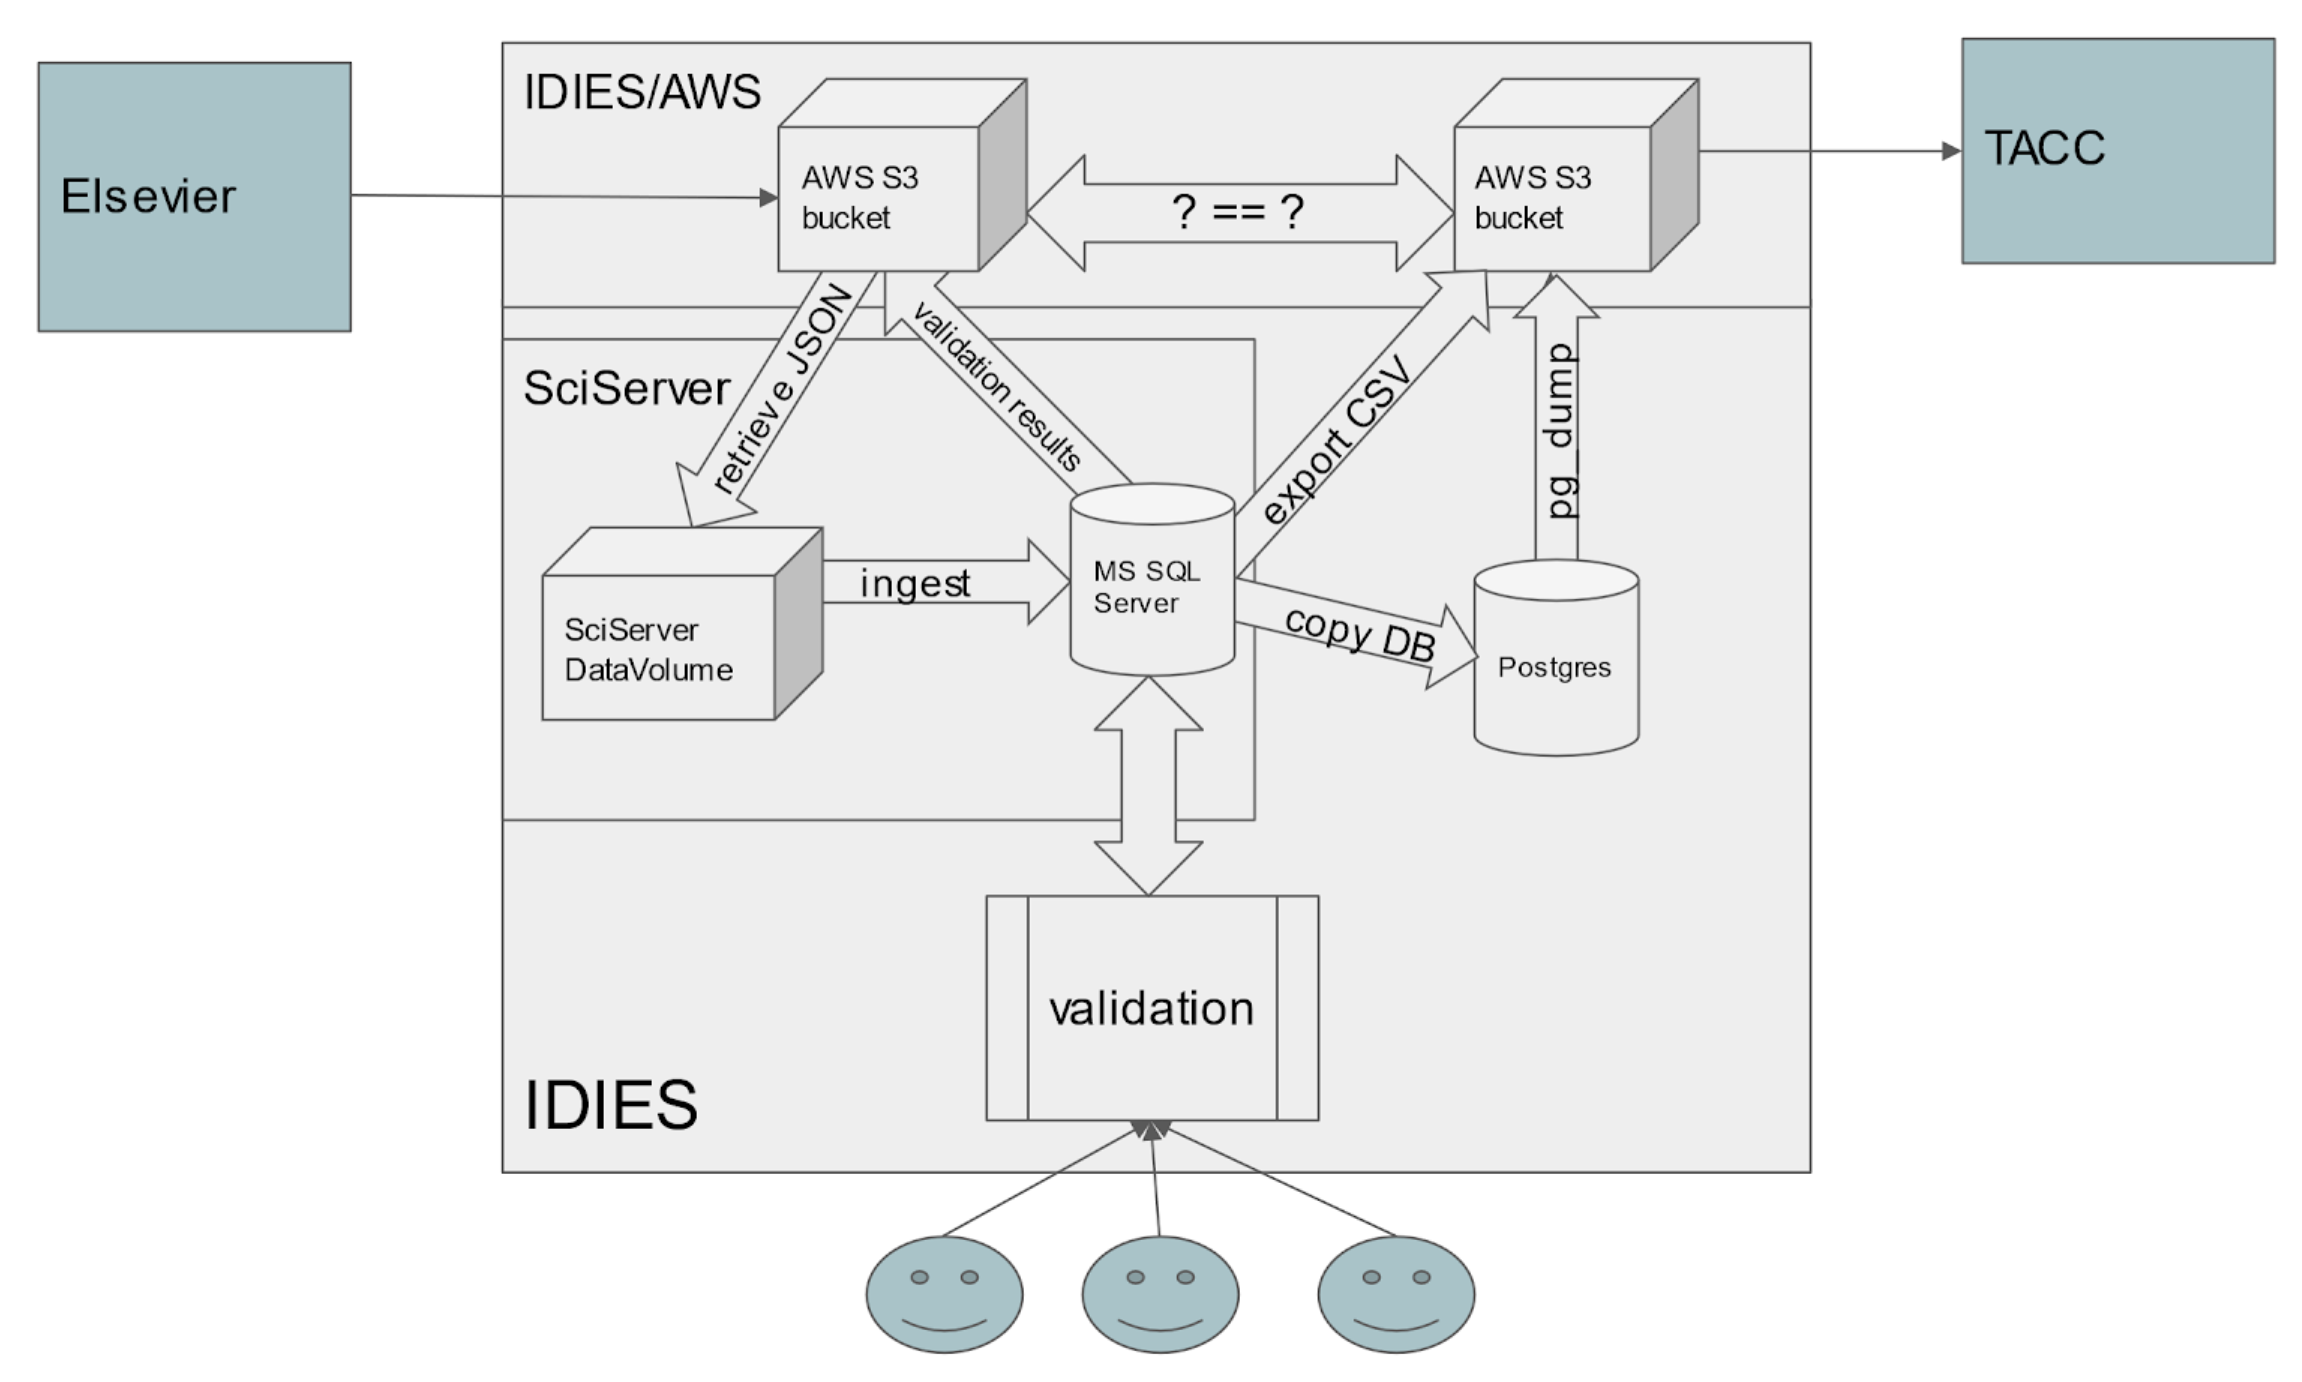
\includegraphics[scale=0.40]{datatransfer.png}
  \caption{Data Transfer Protocol}
  \label{fig:datatransfer}
\end{figure}

\subsection{Validation Tool Specifics}
Each agency has made use of the validation tool to ensure that the ML output is correct. The results: \begin{enumerate}
    \item provide insights into how well the models are identifying datasets, 
    \item find other datasets that are used in conjunctino with the agency datasets to study similar topics, and
    \item identify how researchers make use of each agency's data.
\end{enumerate}

The choice of who will validate depends on each agency.  Many agencies have asked their own subject matter experts to act as validators.  One agency brought in a staff person and made validation one of their tasks. Yet another agency provided funding for a graduate student team from a Hispanic Serving Institution (UT San Antonio) to serve as validators.  Those students are writing a report on their lessons learned that they expect to publish in a scholarly journal and will be active in engaging a diverse community in workshops.

The validation tool is very straightforward, and validators have not hitherto needed training in its use. The tool provides reviewers with snippets from actual publications on which the model has been run and which contain references to the dataset being searched for.  The snippets contain a candidate phrase identified by the model, and the goal is for the validators to determine if these snippets are referring to the correct dataset. 

\begin{description}
\item [Registration.] Validators can’t register themselves in the validation tool. An account is created for them by project personnel, and they will receive their credentials by email. Democratizing Data personnel manage the text snippets that users can review and assign new batches of snippets upon request.   

\item [Sign-in.] The validation tool landing page has a login form for users to sign in.

\item [Review.] When the users log in, they see a bar with the number of snippets assigned and the number of snippets already reviewed. Project personnel initially assign each reviewer a set of snippets to review and can assign additional ones upon request. The reviewers are asked two questions for each snippet:

\begin{itemize}
    \item \textbf{Does the highlighted text in the snippet refer to a dataset?} Confirm whether the machine learning algorithm was correct in considering the phrase as a reference to a dataset in general.
    \item \textbf{Does the highlighted text in the snippet refer to the dataset below?} Confirm whether the model correctly matched the dataset candidate to one of those dataset names provided by the agencies.
\end{itemize}
\end{description}

\begin{figure}
  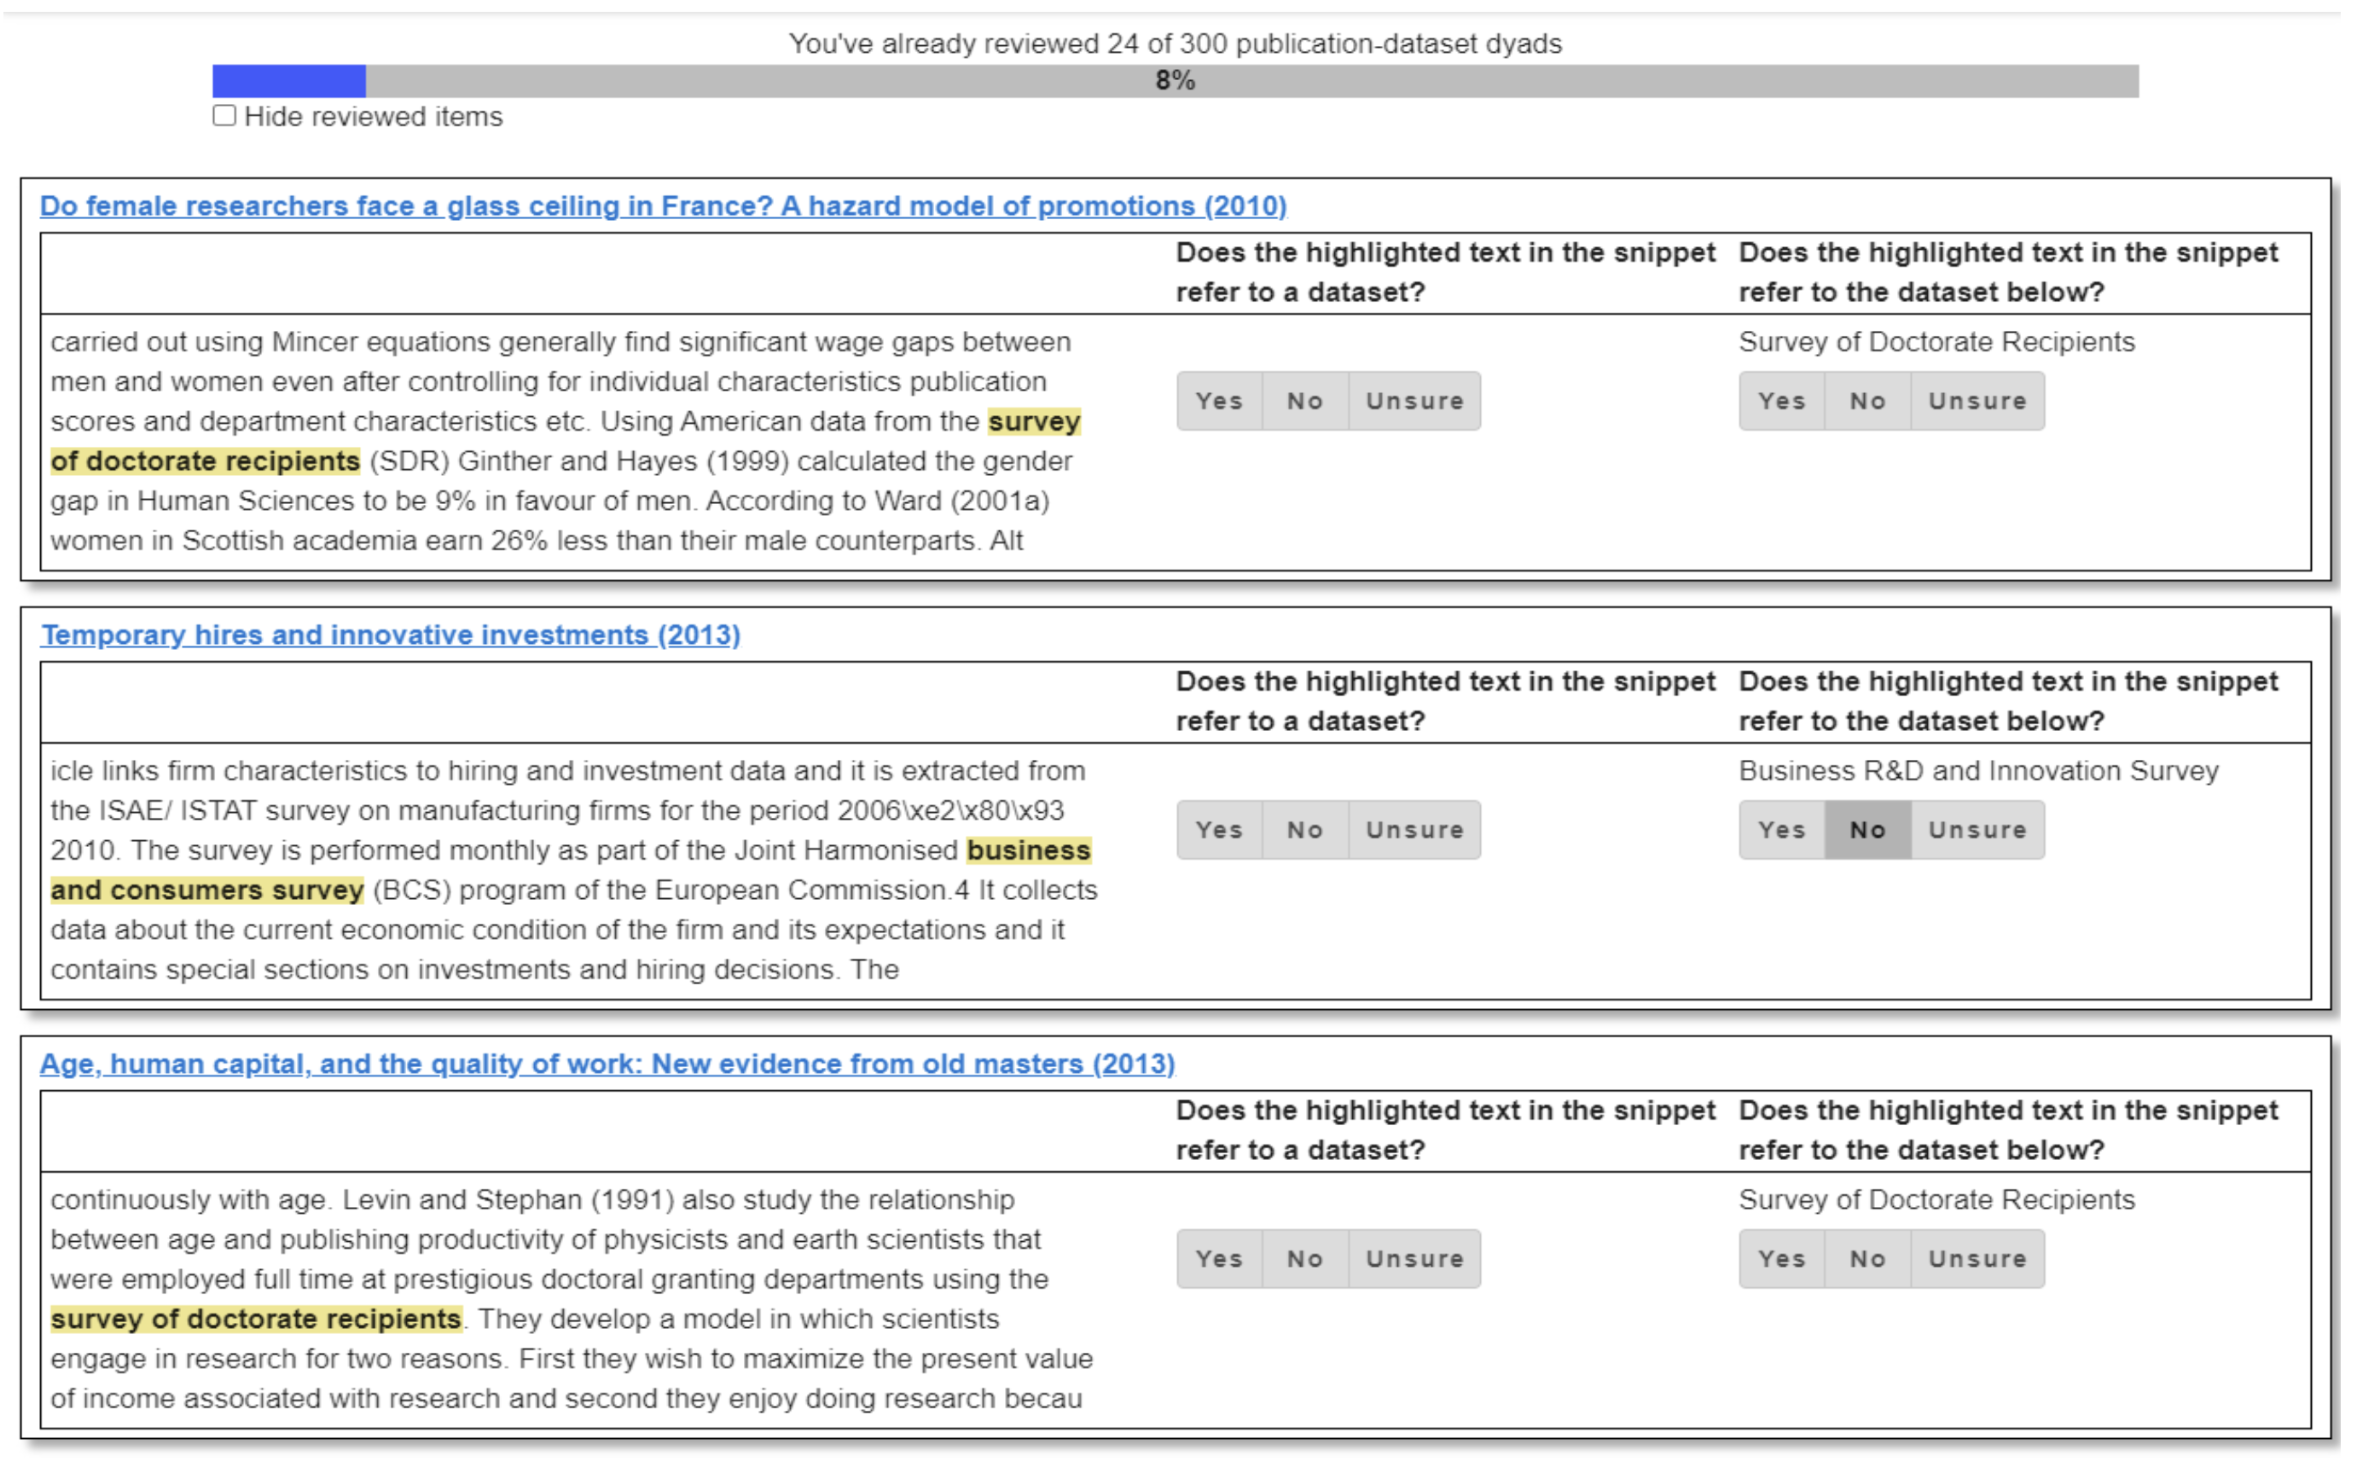
\includegraphics[scale=0.40]{validation_tool.png}
  \vspace{-2.5ex}
  \caption{Screenshot of Validation Tool}
  \label{fig:validation_tool}
\end{figure}

For each question, the reviewer clicks on one box, choosing either yes, no, or unsure. As soon as the users answer the two questions, the text snippet grays out, and they can click the “Modify Review” button to review the text snippet again, changing the answers. Reviewers can also hide/unhide snippets that have already been reviewed by checking/unchecking the checkbox at the top of the page. 

At the very bottom of the page, the users can select the number of snippets per page to display. Only ten snippets per page are displayed by default, and up to 50 snippets per page can be displayed.

\begin{figure}
  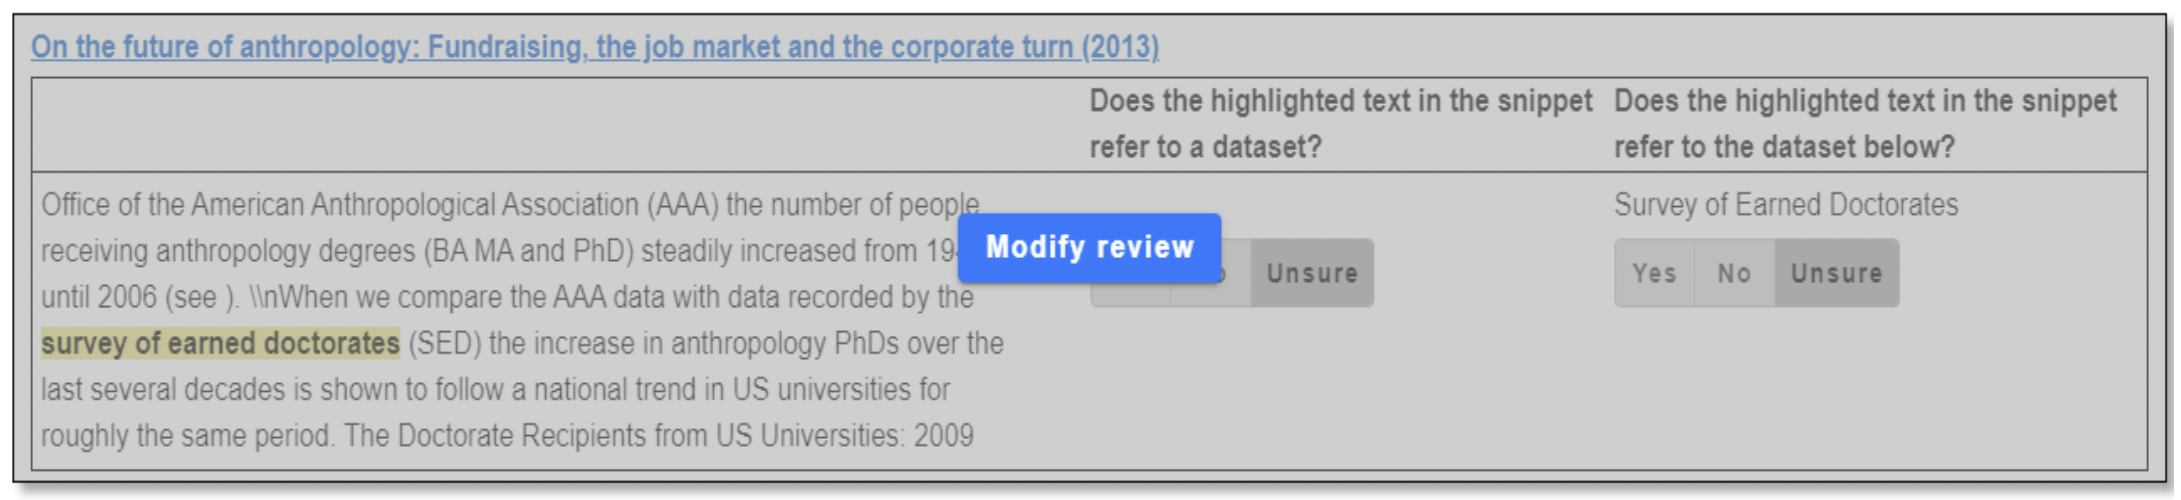
\includegraphics[scale=0.40]{review.png}
  \caption{Screenshot of Reviewed Snippet}
  \label{fig:review}
\end{figure}

Users will see a message thanking them when they review all the snippets on the list. Rich context personnel will assign more snippets to review upon request, and users will receive an email notifying them about the new assignment.

\begin{figure}
  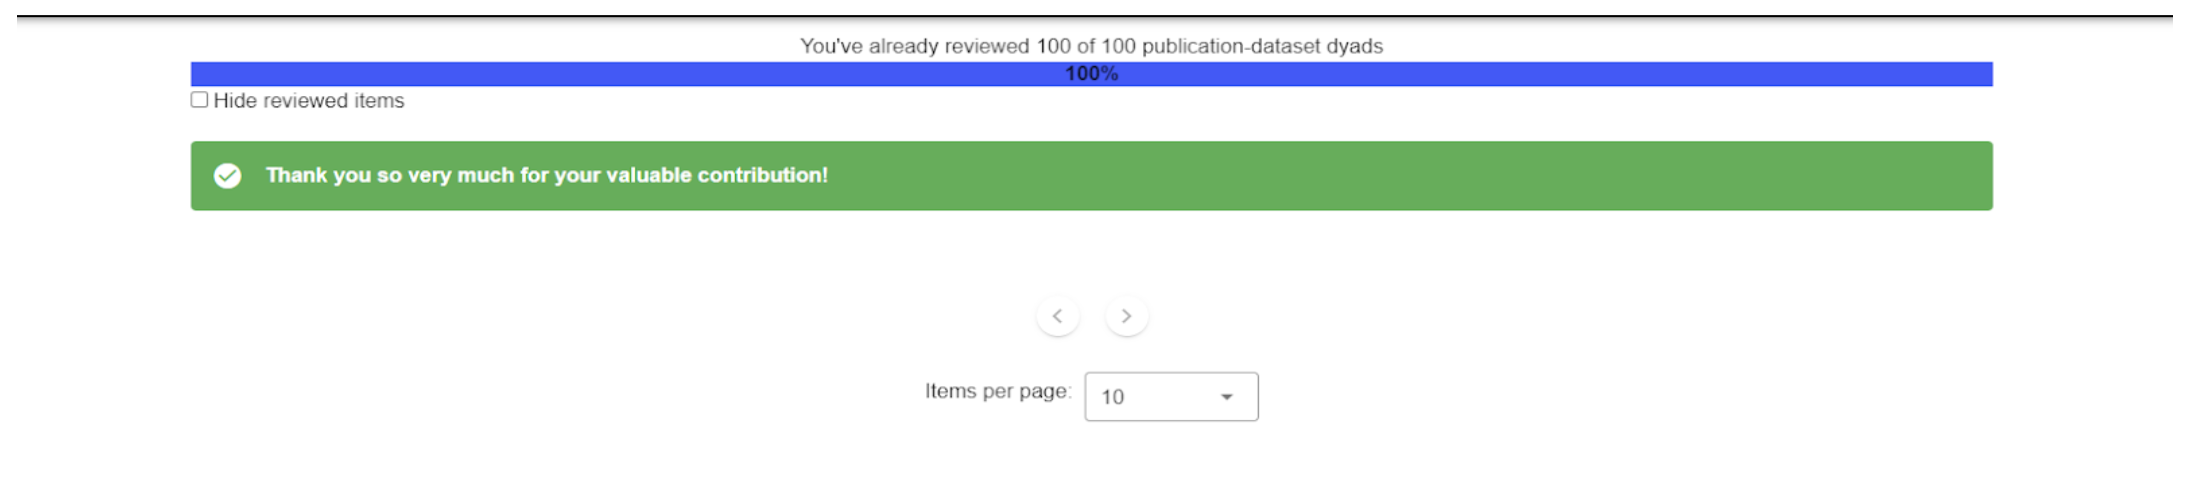
\includegraphics[scale=0.40]{items_per_page.png}
  \caption{Screenshot of Items per page}
  \label{fig:items_per_page}
\end{figure}

\section{JUPYTER NOTEBOOKS AND SCISERVER}
\label{sec:Chapter7}

The Jupyter Notebooks access the database of metadata using an existing successful platform called SciServer. SciServer is built and supported by Johns Hopkins’ Institute for Data Intensive Engineering and Science (IDIES) that builds upon and extends the SkyServer system of server-side tools that introduced the astronomical community to SQL (Structured Query Language) and has been providing the Sloan Digital Sky Survey catalog data to the public\footnote{SciServer uses a Docker/VM based architecture to provide interactive and batch mode server-side analysis with scripting languages like Python and R in various environments including Jupyter (notebooks), RStudio and command-line in addition to traditional SQL-based data analysis. Users have access to private file storage as well as personal SQL database space. A flexible resource access control system allows users to share their resources with collaborators, a feature that has also been very useful in classroom environments. All these services, wrapped in a layer of REST APIs, constitute a scalable collaborative data-driven science platform that is attractive to science disciplines beyond astronomy.}.  It is particularly appealing because, although it was originally designed to support astronomy research, it expanded to include several research and education tools that made access to hundreds of Terabytes of astronomical data easy and intuitive for researchers, students, and the public\cite{source8,source9} . For example, one component of the previous system was Galaxy Zoo, a citizen science project that resulted in reliable classifications of hundreds of thousands of galaxy images – a task that was expected to take multiple staff up to 5 years to complete. In the first Galaxy Zoo, more than 40 million classifications were made in approximately 175 days by more than 100,000 volunteers.\cite{source10}  The current SciServer system has scaled out these tools for multi-science-domain support, applicable to any form of data, including oceanography, mechanical engineering, social sciences, and finance. In addition, SciServer features a learning environment that is being used in K-12 and university education in a variety of contexts, both formal and informal.

\subsection{Accessing SciServer}
The team has developed a fully-fledged schema and data dictionary and developed Jupyter Notebooks that are accessible through SciServer. Users can first register an account at \url{https://apps.sciserver.org} and then contact the team at \href{mailto:sciserver-helpdesk@jhu.edu}{sciserver-helpdesk@jhu.edu} requesting access to Democratizing Data resources, indicating the reasons for the request and their SciServer username.

When access has been granted, example Jupyter notebooks are available on a shared volume alongside the data (see \url{https://apps.sciserver.org/dashboard/files/datavolumes/56} for the base data directory and \url{https://apps.sciserver.org/dashboard/files/datavolumes/56/notebooks} for notebooks). The expectation will be that the user is familiar with the use of Jupyter as an interface, has a basic understanding of scripting (typically in Python), and is comfortable with SQL data retrieval.

\begin{figure}
  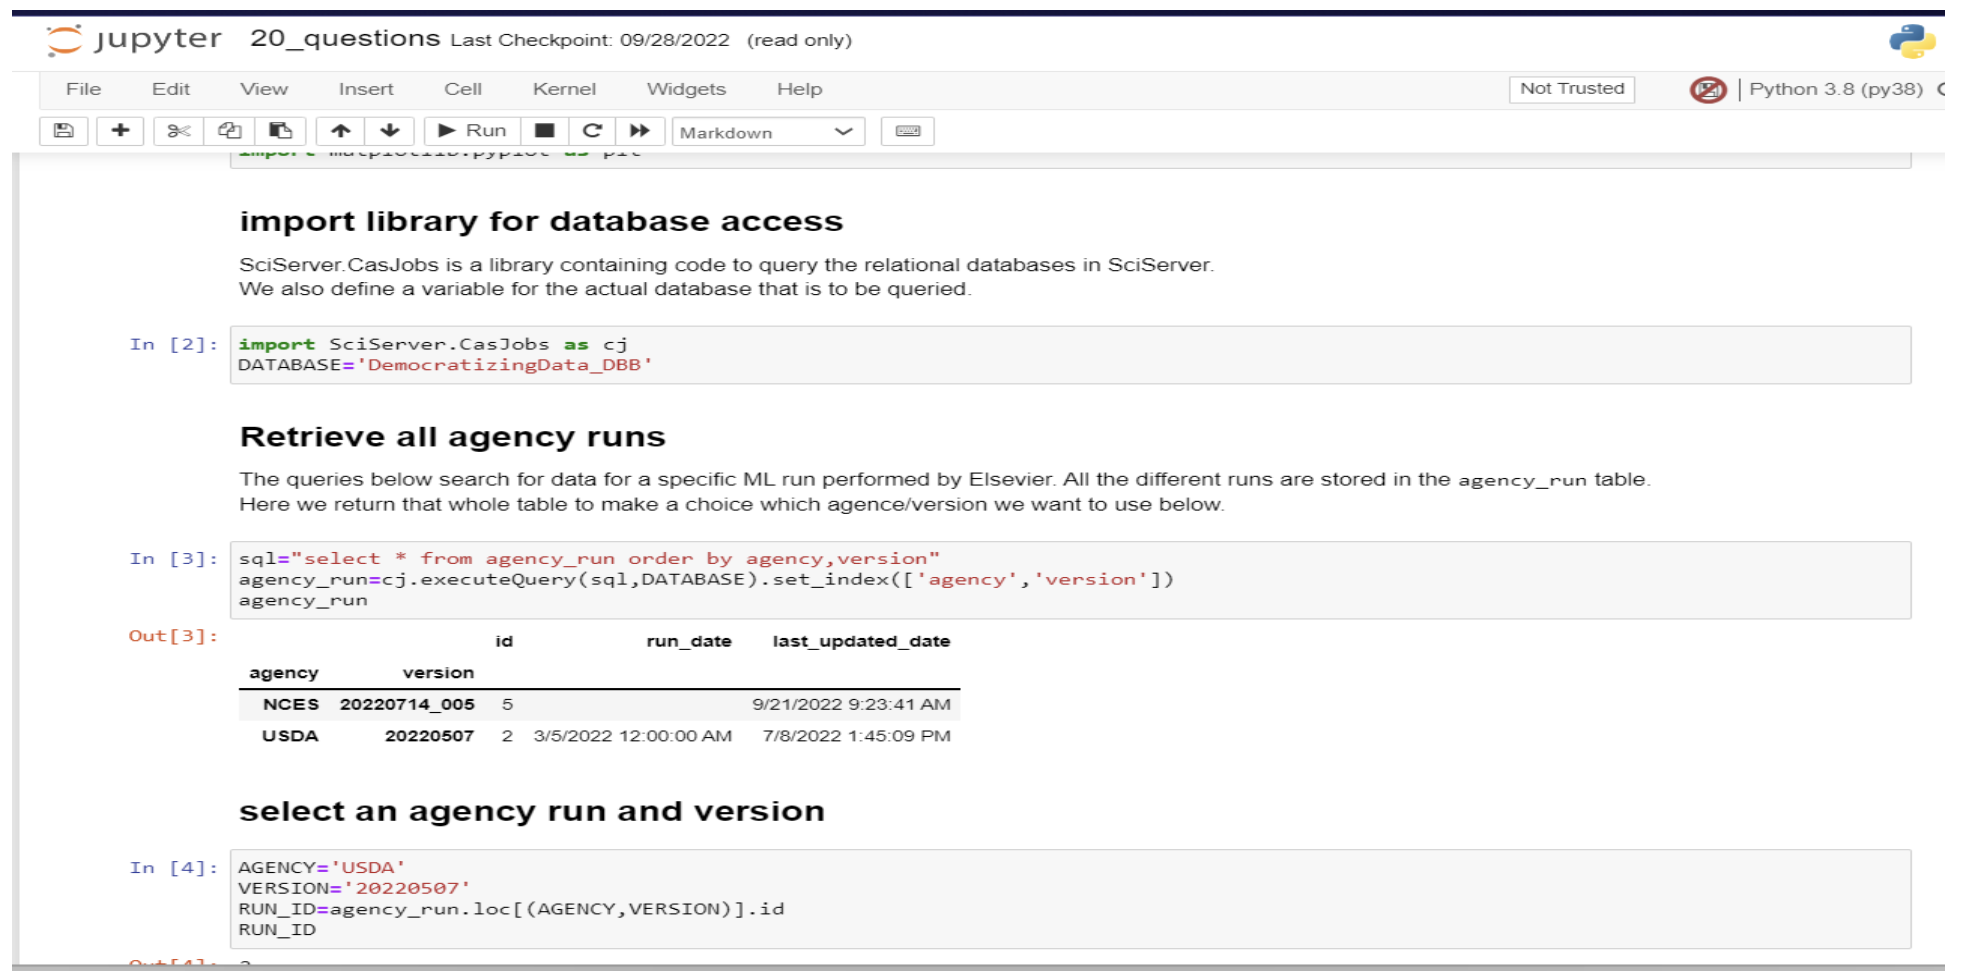
\includegraphics[scale=0.47]{Jupyter_notebook.png}
  \caption{Example of Jupyter Notebook content}
  \label{fig:jupyter_notebook}
\end{figure}


\subsection{Databases on SciServer}

With a SciServer account and the appropriate permissions, a user can query Democratizing Data databases via either the CasJobs interface (see \url{https://www.sciserver.org/about/casjobs/}) or via the CasJobs Python SDK (see \url{https://www.sciserver.org/docs/sciscript-python/SciServer.html#module-SciServer.CasJobs}). 

In addition to a master database (ShowUsTheData\_v3) which contains records for all the agencies processed, there are databases available for individual agencies (possibly containing multiple so-called “runs”) with names of the form “DemocratizingData\_\{AGENCY\_NAME\}”. These agency-level databases provide data in a manner closer to the API (see \hyperref[sec:Chapter8]{Chapter 8}), e.g., validated data without licensed snippet information. Individual users may or may not see some or all of these depending on their access level. For more information on the database schema, please see \hyperref[sec:APPENDIXA]{Appendix A} and \hyperref[sec:APPENDIXB]{Appendix B}.

\section{APPLICATION PROGRAMMING INTERFACE (API)}
\label{sec:Chapter8}
The Application Programming Interface (API) lets agencies and interested stakeholders be able to programmatically pull the metadata and process/display as they wish. Version 2 of the API is currently available to stakeholders and is updated with agency specific data as it is validated and ready for release. 

The API is built using the FastAPI, a Python-based backend which provides routes to database objects with a dynamically generated set of documentation and OpenAPI specifications. The API is containerized and served from Kubernetes and performs calls to functions from the PostgreSQL database. These PostgreSQL function calls optimize query time by making reference to pre-computed database entries in order to decouple query runtime from query complexity. Database updates are propagated to the API via a rollover mechanism that ensures the API will always be performant enough to drive User Interface (UI) applications with minimal downtime. For future capabilities, Fast API can also be integrated with TAPIS (TACC APIs) to provide authentication and fine-grained access controls as needed. 

\subsection{API Prototype}
The prototype Show Us The Data API was a RESTful service that wrapped filter/join functions from the original database schema. The prototype API demonstrated that results from the database could be consumed by external services and clients. The initial prototype was used as an initial springboard for the production API reflected in section 8.2

\subsection{API Version 2}
Version 2 enables two modes of access to the data set.   The first mode supports access for those agency Tableau users who are unable to consume directly from a RESTful API. They can access the data via Web Data Connector and Postgres. The second mode provides access through a RESTful API that supports a generalized Democratizing Data user interface/web client, and provides agencies with the capability of building their own web clients

The Version 2 API includes the following elements:
\begin{itemize}
    \item TACC-hosted PostgreSQL database that retains production ready, validated data within tables. For complex queries, materialized views are used to maintain query performance;
    \item Web Data Connect that allows Tableau to retrieve data from the production Postgres Tables and materialized views;
    \item Production, Pre-production and Development Postgres instances, with access for Democratizing Data to develop and push data directly to the Postgres environment with a rollover-based deployment process for new production data and schema changes;
    \item (In progress) Automated testing to ensure endpoints and producing proper data when new agency information is pushed to the API;
    \item (In progress) Landing page for agencies that will answer high level questions and provide further information on how to access additional detailed data.
\end{itemize}

API endpoints are dependent on what the new data set schema is capable of providing, with requirements for additional endpoints flowing to the Democratizing Data schema team in an iterative development process. The current endpoints are listed in the OpenAPI specification, many of which currently support the “main questions” requirements. These are documented at \url{https://democratizing-data.tacc.utexas.edu/docs} as well as here \url{https://prod.democratizing-data.tacc.utexas.edu/redoc}  and  \url{https://prod.democratizing-data.tacc.utexas.edu/docs#}

\section{USAGE DASHBOARD}
\label{sec:Chapter9}
Beyond offering an API, the platform currently provides a prototype usage dashboard that enable agencies to visualize answers to \hyperref[subsec:Agencyquestions]{agency questions}. The initial example for USDA can be viewed \href{https://public.tableau.com/app/profile/democratizing.data/viz/DemocratizingData-WebDataConnector-USDA-NewLayout/Publications}{here}.

As the project evolves, and agencies share resources, it is expected that new dashboards will evolve, as USDA/NASS has shown with their approach \href{https://public.tableau.com/app/profile/national.agricultural.statistics.service/viz/5WsofNASSDataUsage/The5Ws}{here}. The proposed production version for a common agency baseline website is in wireframe stage and described in the following sections.

\subsection{Basic Usage Information}

The initial agency landing page will provide basic usage information, as required by the Foundations of Evidence-based Policymaking Act.  Agencies have asked that the landing page provide information about how much agency datasets are used in research and how has that usage changed over time.  

% TODO: insert image "figure 9"
\begin{figure}
\centering
  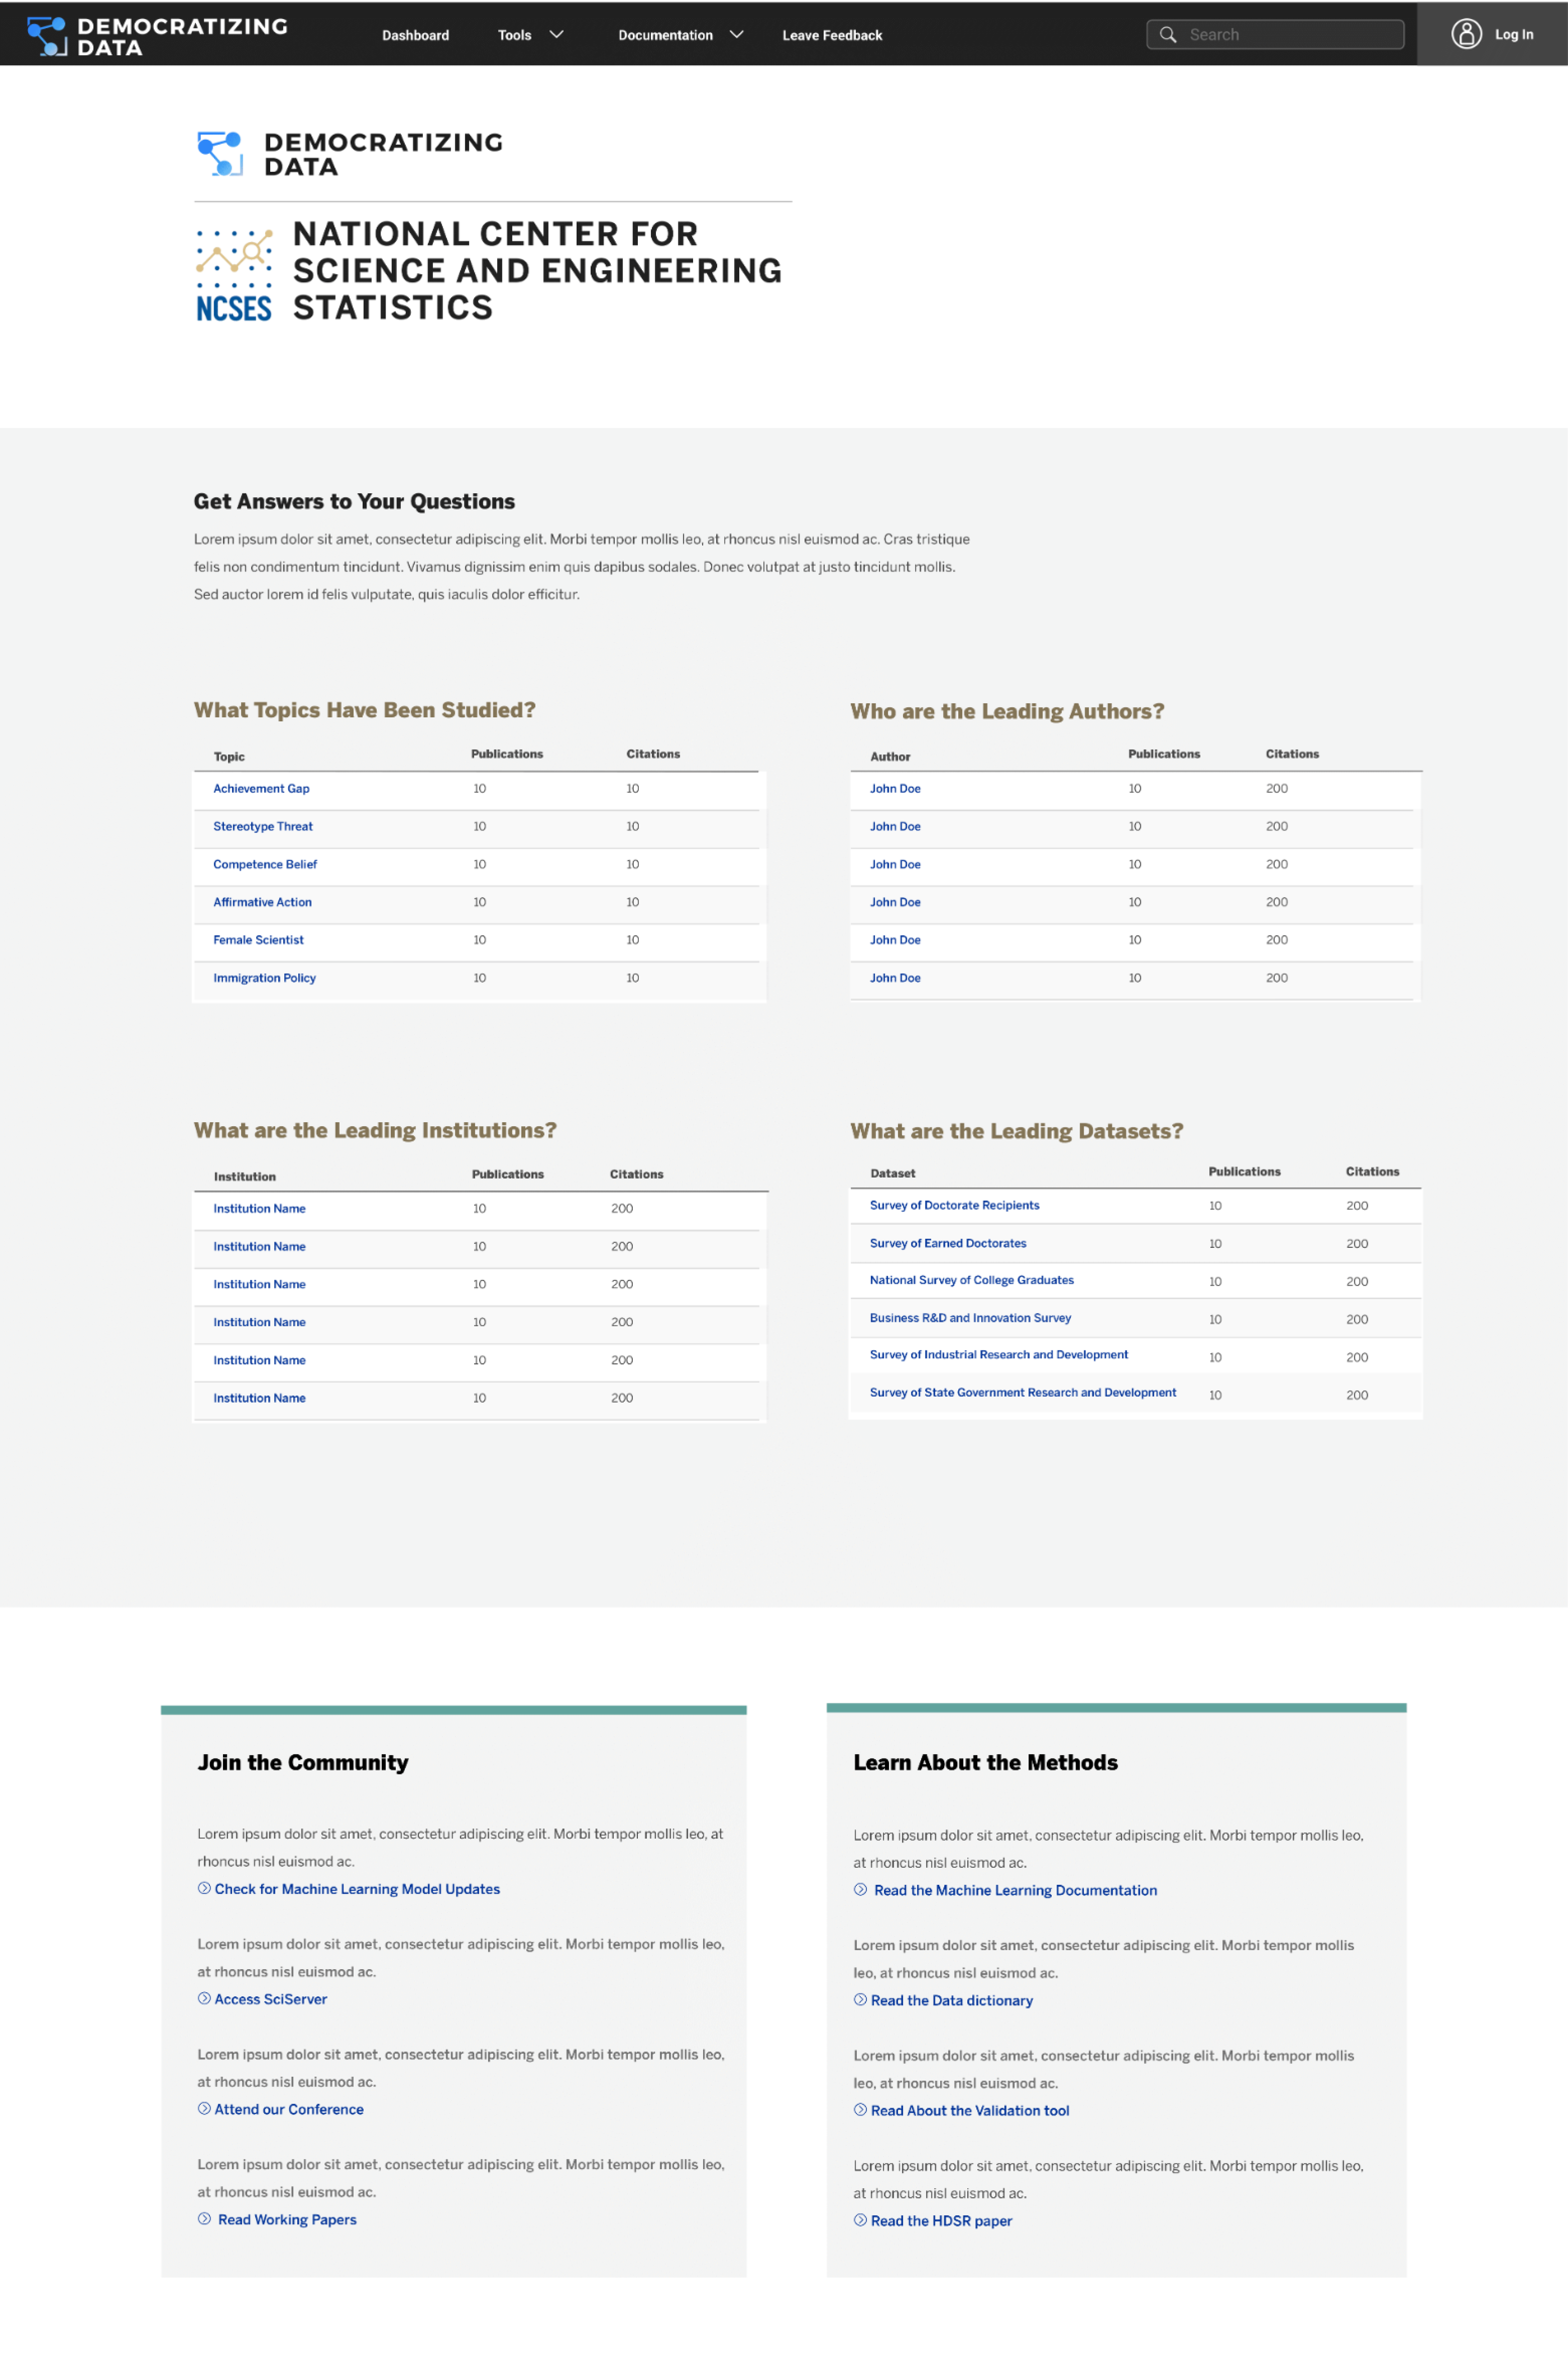
\includegraphics[scale=0.25]{agency_landing_page.png}
  \caption{Agency landing page (NCSES example)}
  \label{fig:agency_landing_page}
\end{figure}

\subsection{Portfolio Information}
Agencies have also asked for reports about their portfolio: i.e., how their data are used.   Their questions include: What topics are agency datasets being used to study, and what publications are associated with each topic? What topics are each one of an agency’s identified dataset used in research and what publications are associated with each topic? What other datasets are being used to study each topic?  \hyperref[fig:review]{Figure 8} shows the answers to those questions.
% TODO: insert image "figure 10"
\begin{figure}
\centering
  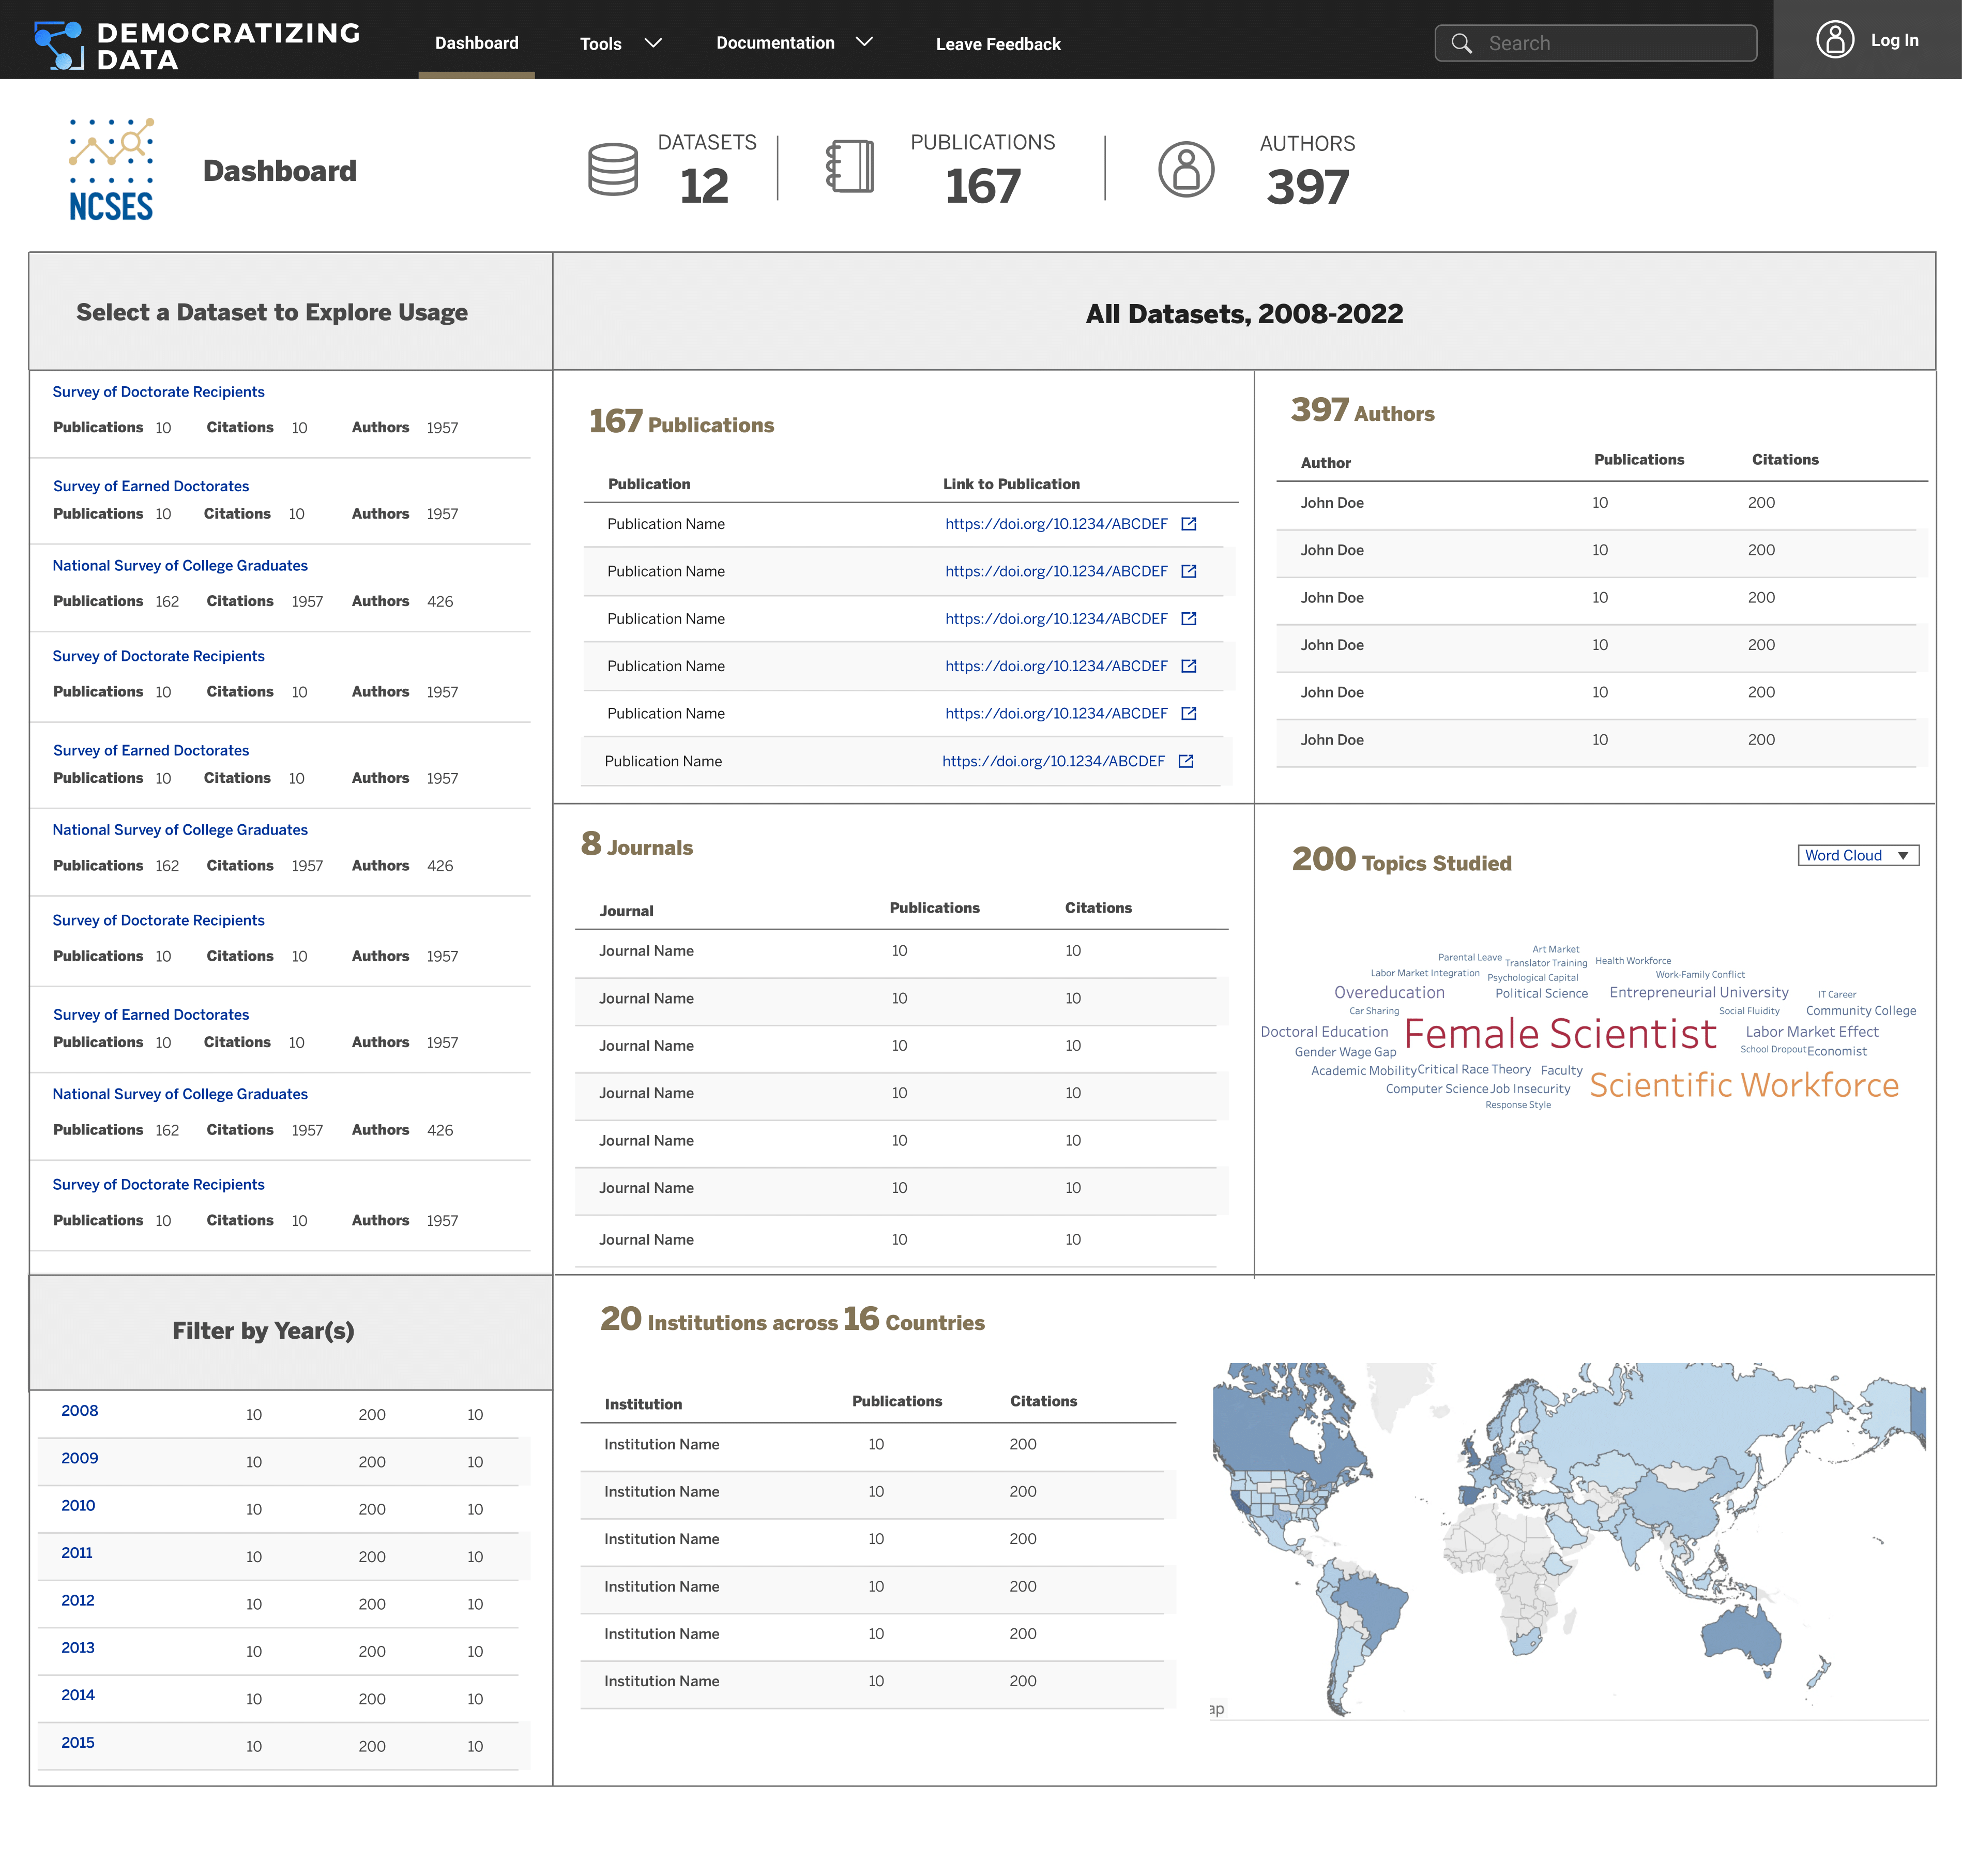
\includegraphics[scale=0.30]{portfolio.png}
  \caption{Portfolio information}
  \label{fig:portfolio}
\end{figure}

\subsection{Drilling into details}
Agencies have also requested information that can also be used by researchers about each dataset in their portfolio, as shown in \hyperref[fig:items_per_page]{Figure 9}.  They have specific questions and the goal of these dashboards is to provide an easy-to-use and clear to understand interface to answer the most pressing questions. Their questions include: who are the main authors using each agency’s datasets?  Who are the main authors using each dataset, and the associated publications? What institutions are the centers of use for each agency dataset and in what geographic locations are the institutions located?  What are the journals publishing work using the dataset?

% TODO: insert image "figure 11"
\begin{figure}
\centering
  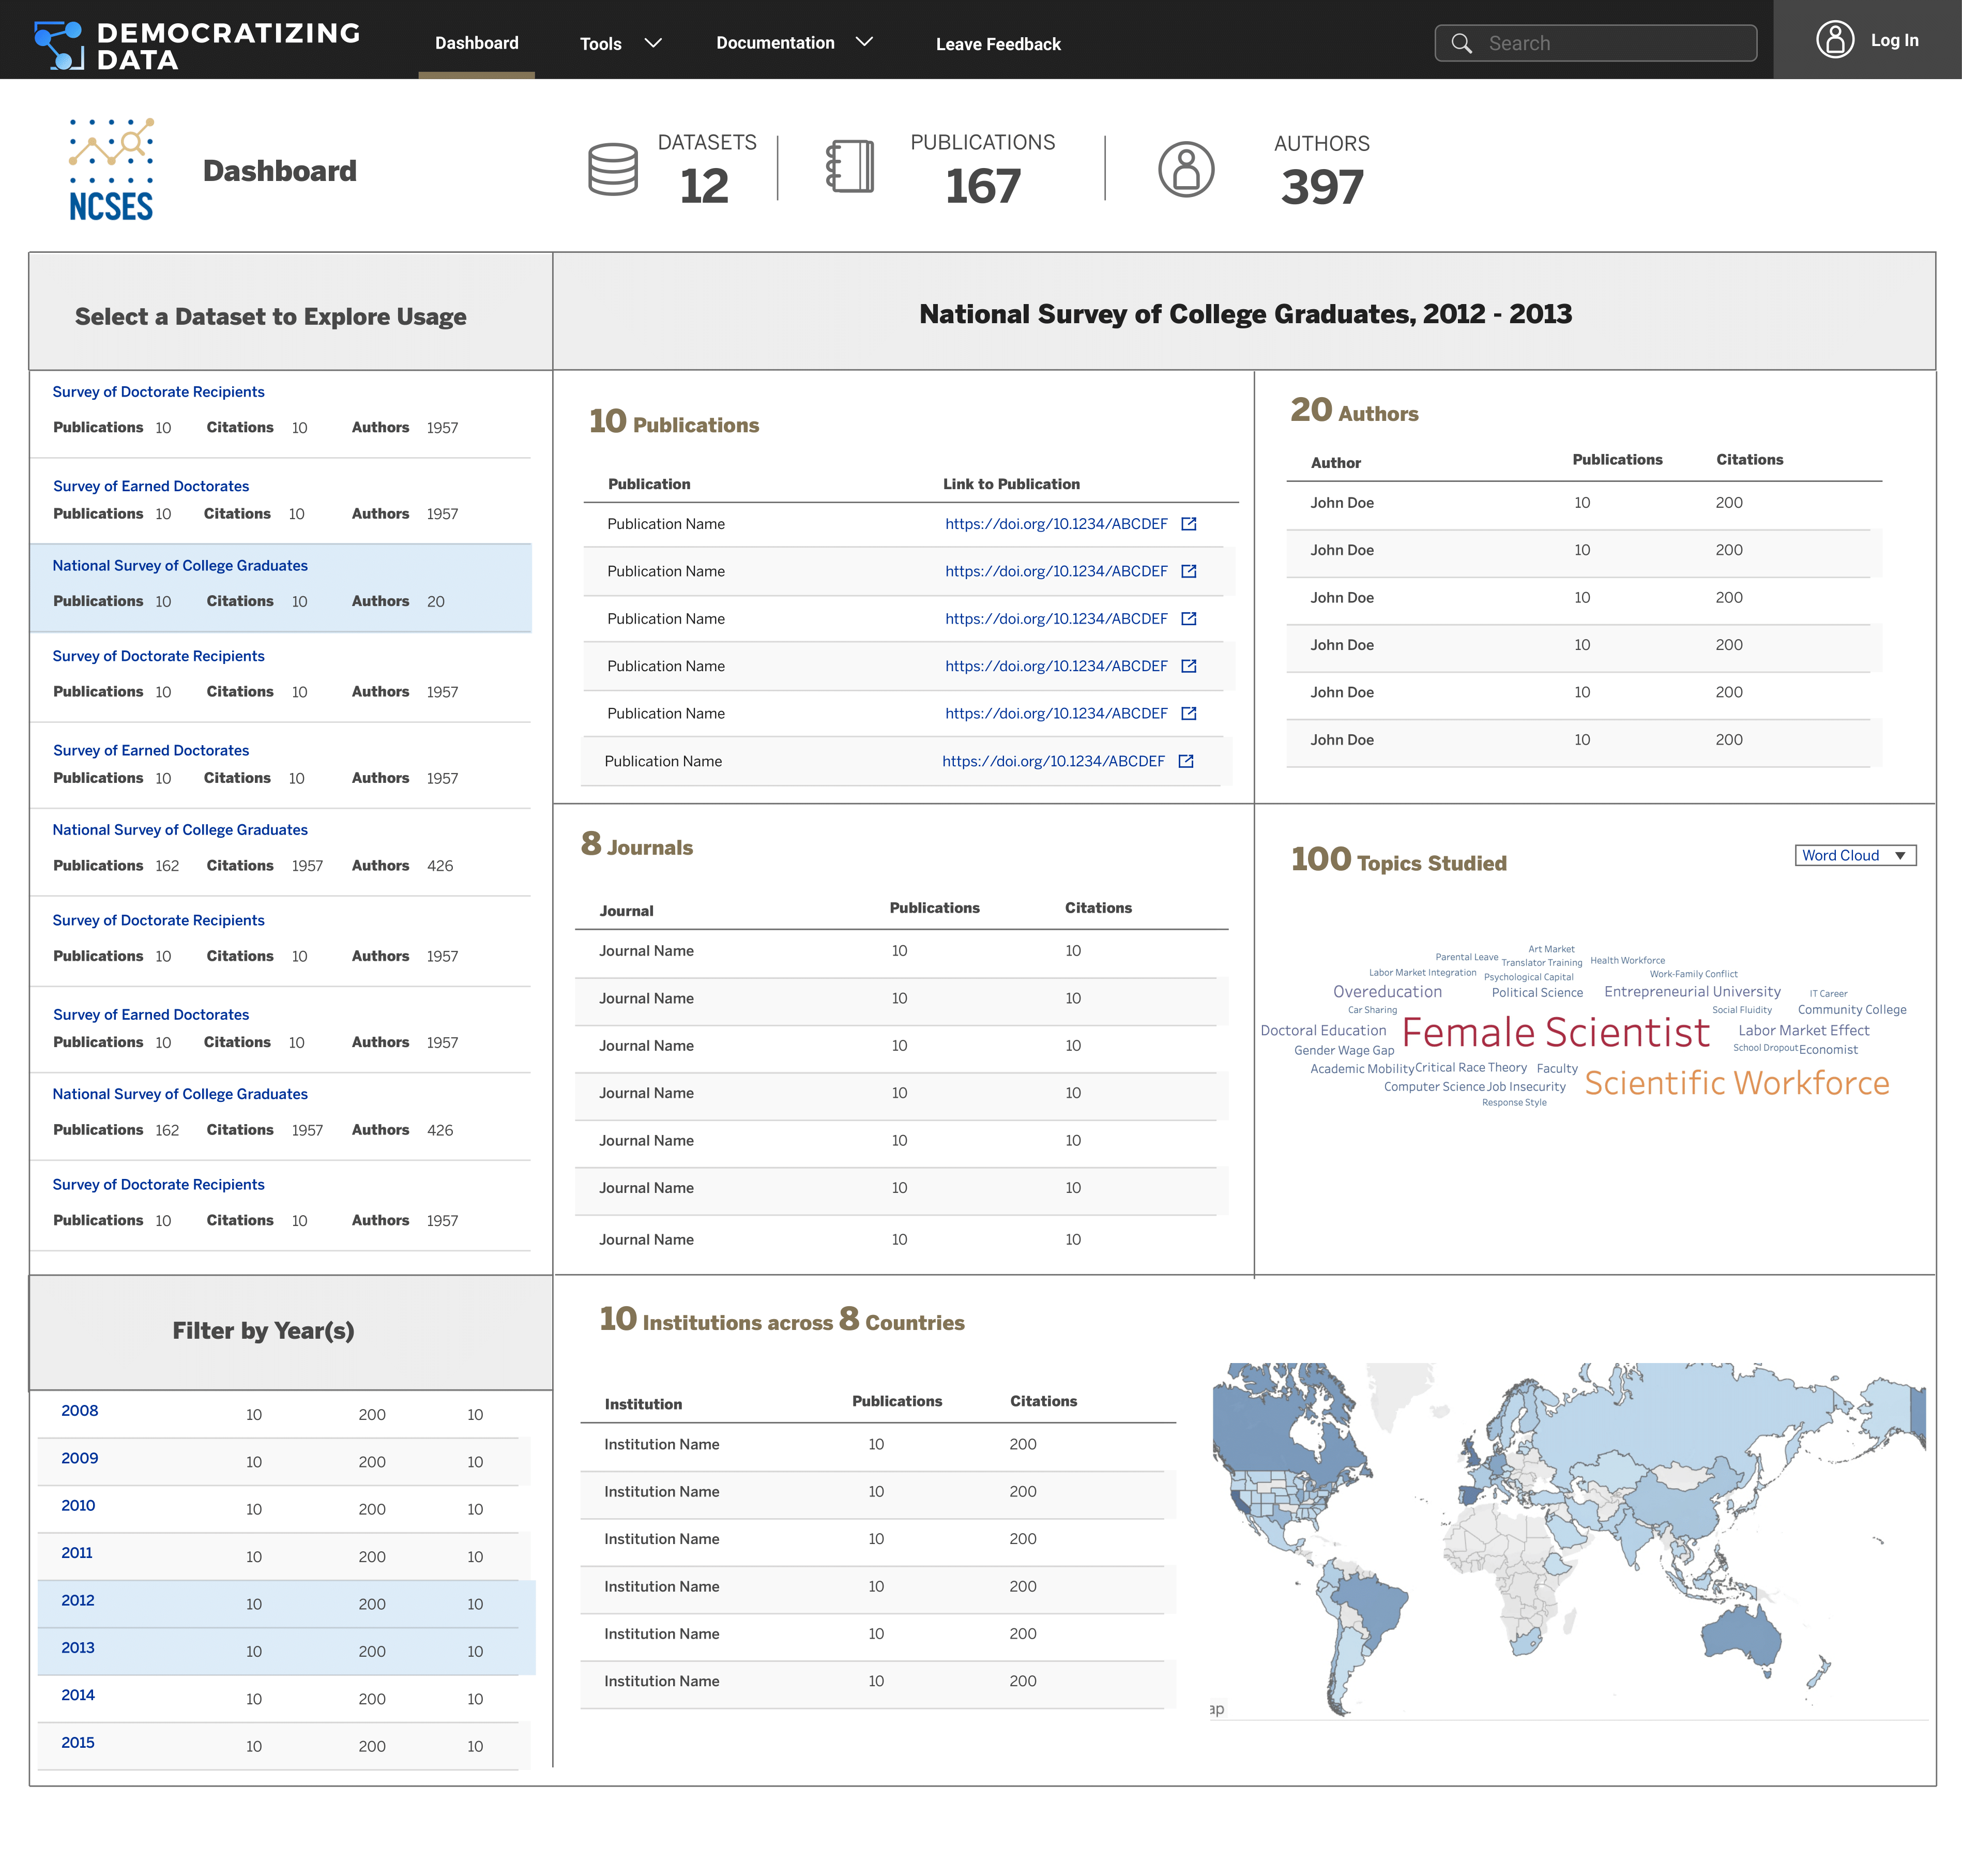
\includegraphics[scale=0.30]{Researcher.png}
  \caption{Researcher dashboard with dataset specific information}
  \label{fig:Researcher}
\end{figure}

\section{DASHBOARD FOR NETWORK EXPLORATION}
\label{sec:Chapter10}
In addition to the researcher dashboard and the access to the database using the Jupyter Notebooks in SciServer, the team is also developing other user-friendly tools using Jupyter Notebooks. The most developed is the Dashboard for Network Exploration, which has been designed to visualize and explore network graphs derived from the target  datasets, and to visualize tables with their associated metadata. 

\subsection{Accessing the Dashboard}
The dashboard can be accessed through 2 different interfaces:
\begin{itemize}
    \item Standalone website: \url{https://showusthedata.idies.jhu.edu/dashboard/} (does not require login).
    \item Within SciServer in a Jupyter Notebook (requires login).
\end{itemize}


% TODO: insert image "figure 12"
\begin{figure}
\centering
  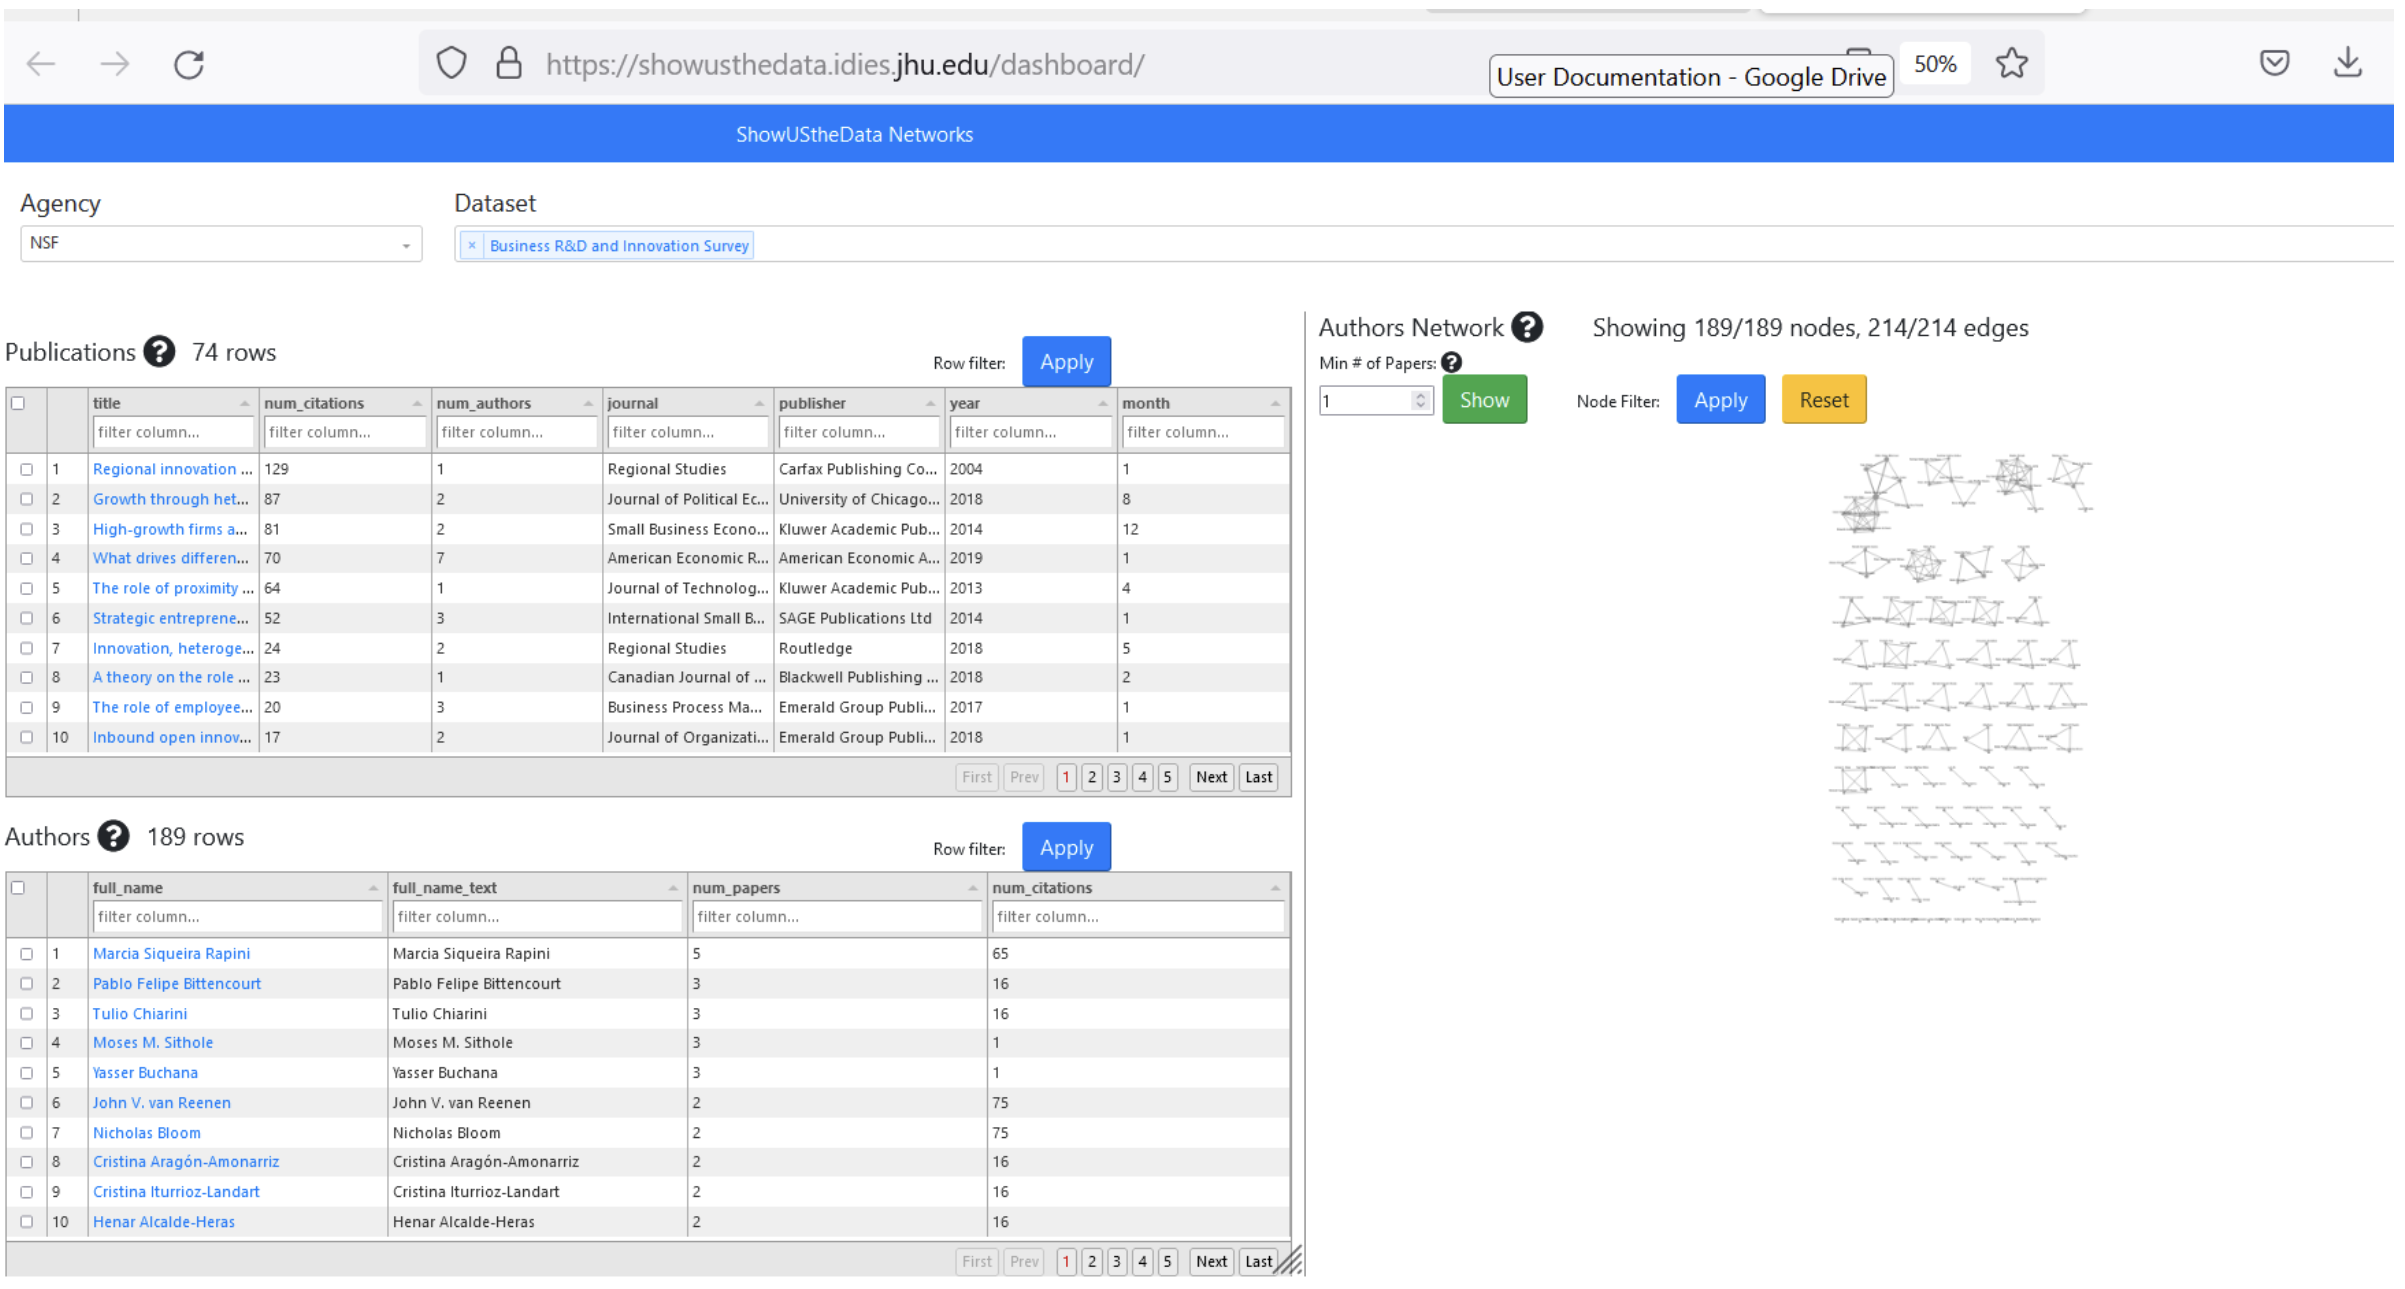
\includegraphics[scale=0.40]{network.png}
  \caption{Network Visualization screenshot}
  \label{fig:network}
\end{figure}

\subsection{Dashboard Filters}
The notebooks provide filtering capabilities, where filtering on the network nodes will filter out their associated rows in the metadata tables, and vice-versa.

\begin{description}
\item [Author.] The nodes of the network are the publication authors.

An edge (link) connecting 2 author nodes is created if those authors appear in the same publication. The size of a network node is proportional to the number of papers published by each author. The width of the edge connecting 2 authors is proportional to the number of papers they have published together.

\item [Institutions.] The nodes of the network are the institutions of publication authors. An edge (link) connecting 2 institution nodes is created if an author from one institution appears in the same publication as an author from the other institution. The size of a network node is proportional to the total number of publications associated to the institution. The width of the edge connecting 2 institutions is proportional to the number of publications their authors have published together.

\item [Topics.] The nodes of the network are the topics related to publications.  An edge (link) connecting 2 topic nodes is created if the 2 topics appear in the same publication. The size of a topic node is proportional to the total number of times it appears in all publications. The width of the edge connecting 2 topic nodes is proportional to the number of publications the topics have in common.

\end{description}

The following tables and respective columns are shown on the left half of the screen:

\begin{itemize}
    \item \textbf{Publications}: title, journal, publisher, year, month, number of citations and authors. The title column is clickable and opens the journal web page with information about the publication.
    \item \textbf{Authors}: name, number of papers and citations. The name column is clickable and opens the scopus web page with information about the author.
    \item \textbf{Topics}: name, number of papers and citations. Topics are related to the publication, as defined by Elsevier.
    \item \textbf{ASJCs}: name, number of papers and citations. These are ALL Science Journal Classification codes assigned to the publications. 
    \item \textbf{Journals}: name, number of papers, and citations.
    \item \textbf{Datasets}: name, number of papers, citations, and authors.
    \item \textbf{Agencies}: name, number of papers, citations, and authors.
    \item \textbf{Institutions}: name, city, country, number of papers, citations, and authors.
    \item \textbf{Countries}: country name, number of papers and citations.
    \item \textbf{Yearly Statistics}: year, number of citations and papers per year.
\end{itemize}

% TODO: insert image
\begin{figure}
  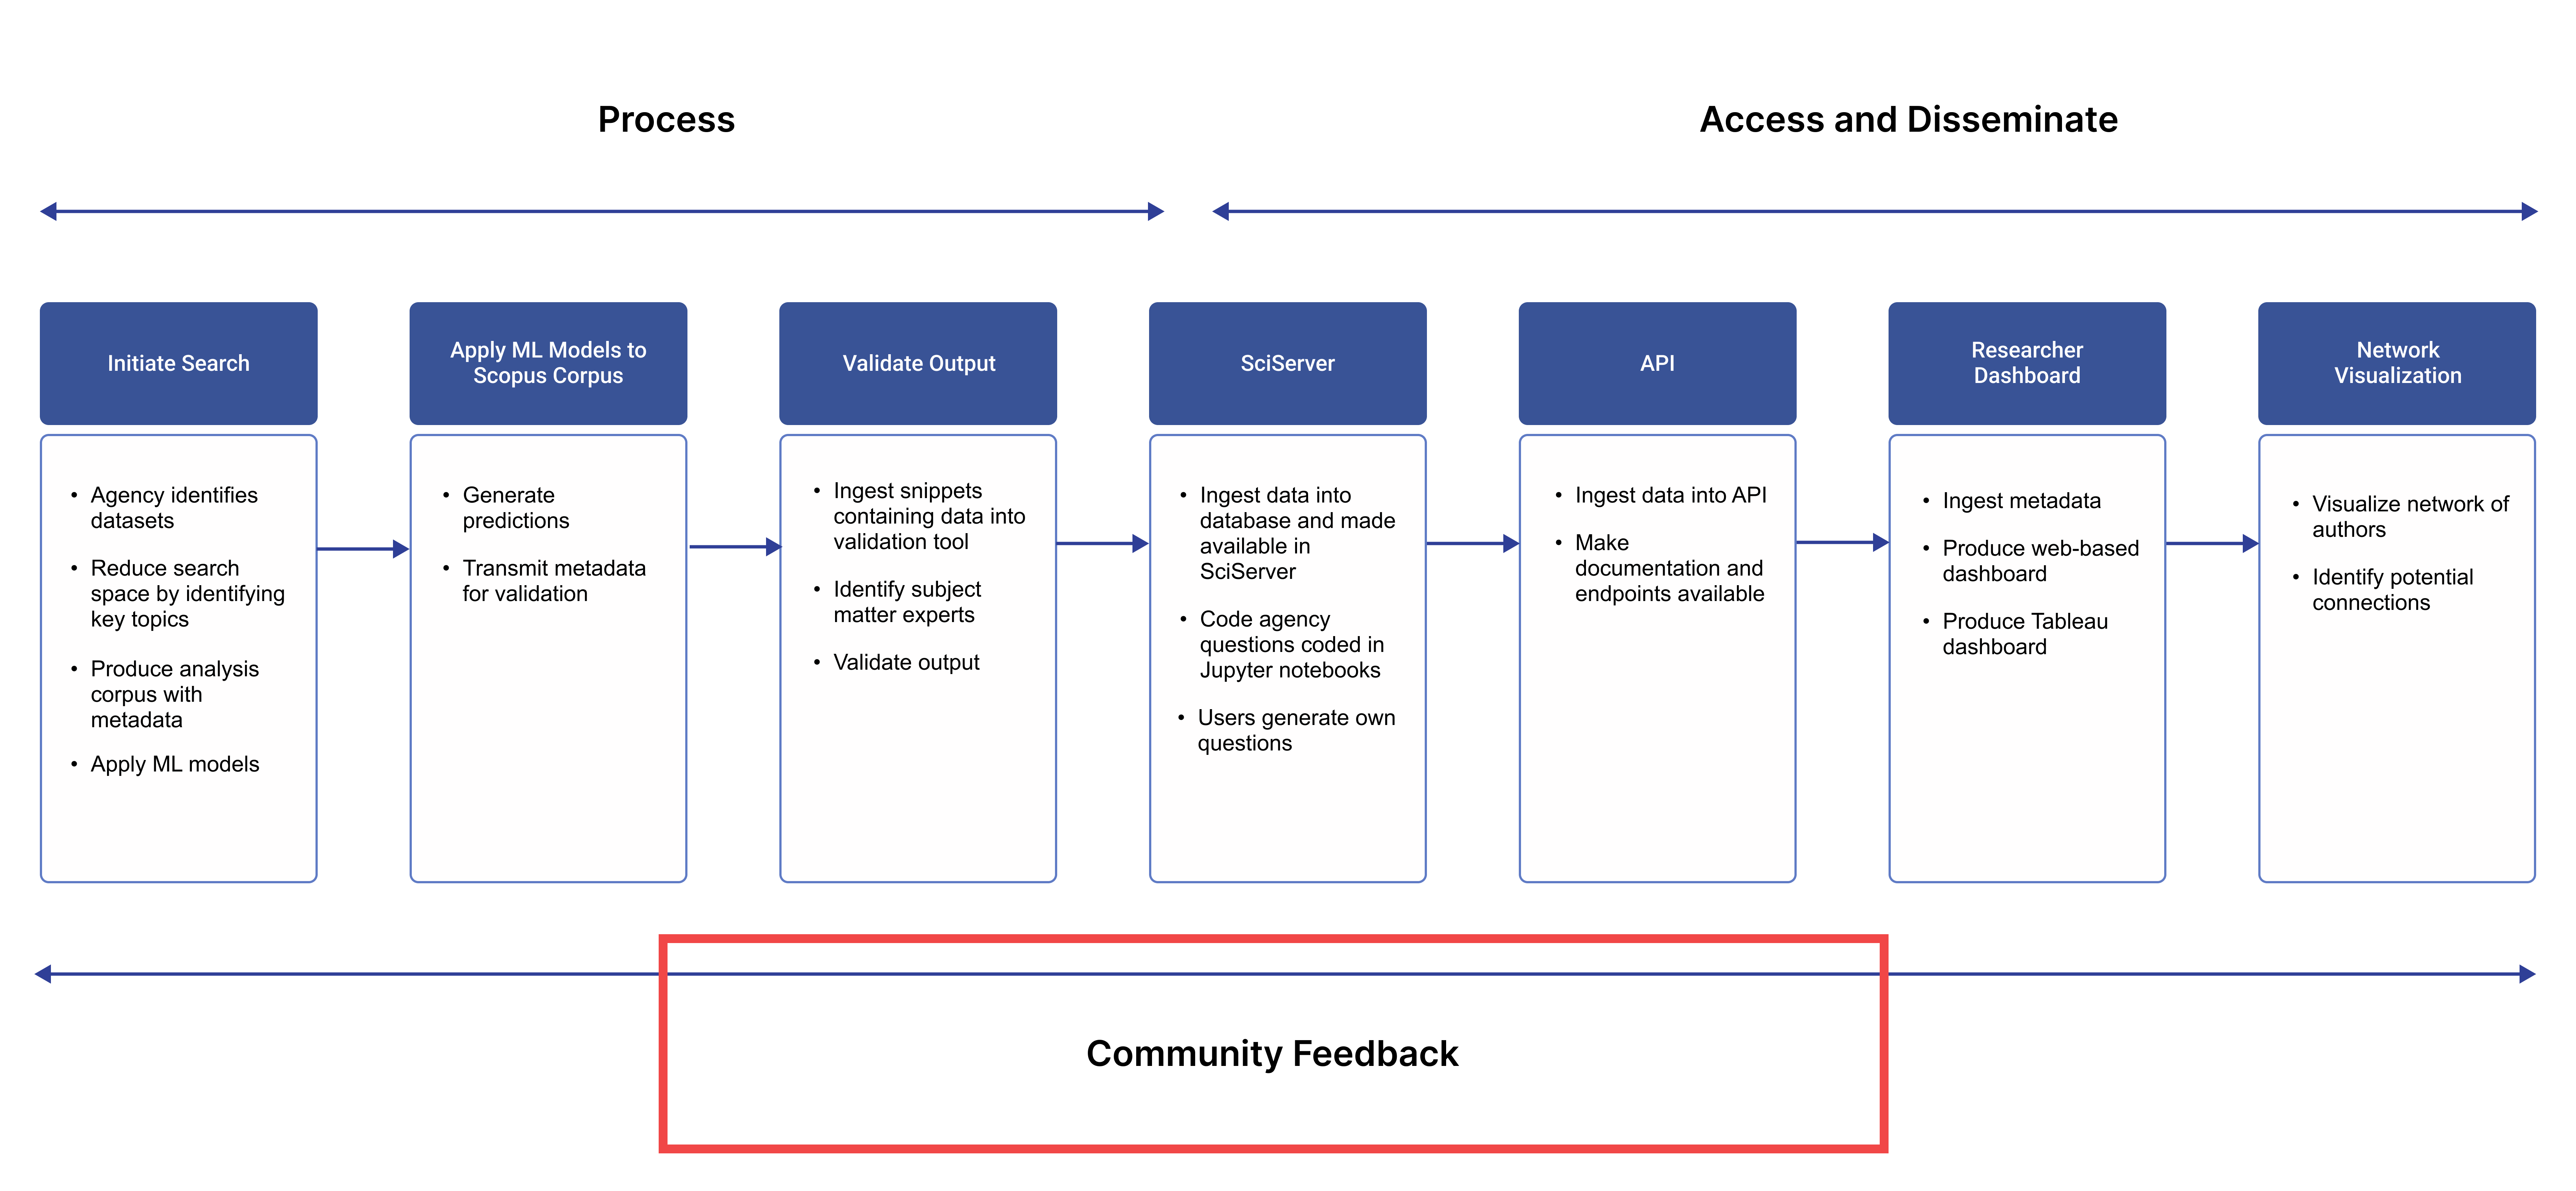
\includegraphics[scale=0.20]{Feedback.png}
  \vspace{-2.5ex}
  \caption{Community Feedback}
    \vspace{-0.97ex}
  \label{fig:feedback}
\end{figure}


\section{COMMUNITY OUTREACH AND ENGAGEMENT}
\label{sec:Chapter11}
One of the key goals of the project is to ensure that the user community – both internal to the agency and external – is engaged in substantive ways through workshops, webinars, and a dedicated website that provides opportunity for comment and feedback. Such engagement is not only mandated by the legislation identified in \hyperref[sec:Response to Legislative Mandate and Committee Recommendations]{Section 2.3}, but also often recommended by National Academies report\footnote{Such as, for example, the CNSTAT report on “\href{https://www.nationalacademies.org/our-work/a-vision-and-roadmap-for-education-statistics-in-2030-and-beyond}{A Vision and Roadmap for Education Statistics}” }.

While each agency will have its own way of engaging with its internal constituents, there are some common threads that could shape the external engagement with researchers, survey respondents, data users, and specific under-represented groups. However, it is expected that each agency will identify the target user community to participate in the early workshops. 

The general format of a user community early workshop would be to explain the platform, provide hands-on experience using Jupyter Notebooks, and to gather feedback on: \begin{enumerate*}
    \item how to improve the functionality of the platform;
    \item usability of the platform; and
    \item future possible collaborations between the agency and the user community and within the user community.
\end{enumerate*}

Multiple workshops could be structured to serve the different potential constituencies. One might focus on survey respondents, who would react to the usage information in the dashboard. Another might focus on users of the Standard Application Process for the Federal Statistical Research Data Centers. A third might include graduate students, postdocs and other junior scholars who have yet to develop the connections to the empirical knowledge base in a research field. 

The workshops will include participation from all the project partners but will primarily be supported by University of Maryland, NYU, and the agencies. The partners are committed to working with the agencies to bring in a diverse and inclusive range of participants, particularly from academic institutions such as Historically Black Colleges and Universities and Hispanic Serving Institutions.

Subsequent workshops could provide input into the theory of change – how investing in data creates value. That theory of change can provide the framework for developing well grounded usage metrics and inform the development of agency questions.  As such, a researcher engagement workshop might bring together both active and potential data users, senior and junior researchers interested in the agency mission areas, as well as evaluation experts.

It is also possible that subsequent workshops include the broader federal community. The Evidence Act requires that agencies engage with the user community, and charged three key federal entities with fulfilling that task.  These include statistical officials (through the Interagency Committee on Statistical Policy), Chief Data Officers (the Chief Data Officer Council) and Chief Evaluation Officers.  

\subsection{Other Outreach}
Other outreach activities are likely to include presentations at professional conferences of researchers and data users, presentations to federal cross-agency councils, such as the Chief Data Officers Council and the Interagency Council on Statistical Policy, and associations such as the Council of Professional Associations on Federal Statistics.  Each agency will be at the center of planning for their outreach activities, with support from the partners. 

\subsection{Learning from Previous workshops and Outreach}
Much previous work can be used in designing the workshops. The Show Us the Data workshop provides a strong basis, since information (reproduced below) was provided by Chief Data Officers, the research community, publishers, and academic institutions.

% why is this just hanging here
\href{https://coleridgeinitiative.org/show-us-the-data/stakeholder-questions/#federal-agencies}{Chief Data Officer and Evidence Officials}

Since the competition focused on uses of data sets in research, the outcomes were most immediately appliable to agencies with scientific mission components. CDOs from agencies for which discovery activities occurred in the competition were invited to review results in one-on-one sessions and then to attend this panel discussion.  The Agencies represented in the discussion were Commerce (NOAA), NSF, USDA, Transportation.   Given that the breadth of data work in an Agency may cross many mission teams, some agencies had multiple team members participate in the discussion session Their detailed responses are summarized in \hyperref[subsec:CDOE]{Appendix D: CDOS}.

% TOD0: insert figure 13
\begin{figure}[t]
\centering
  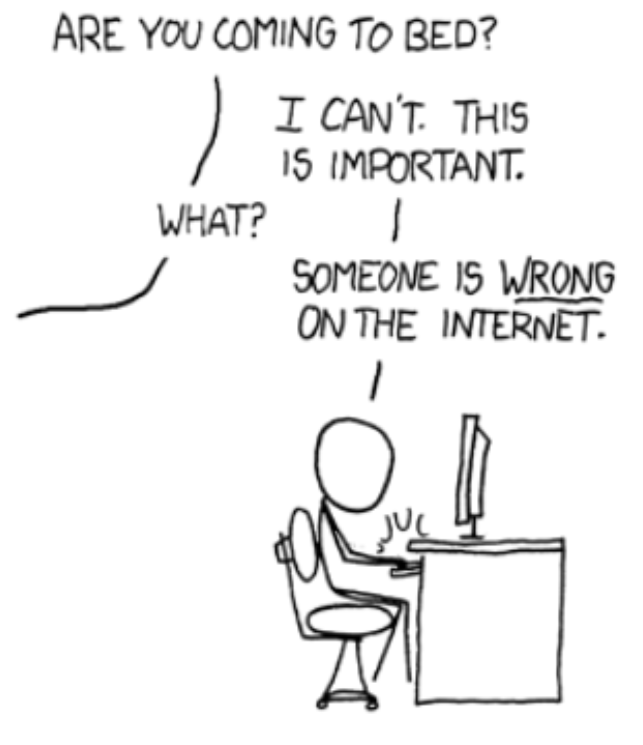
\includegraphics[scale=0.50]{error.png}
  \caption{Error correction}
  \label{fig:error}
\end{figure}


\href{https://coleridgeinitiative.org/show-us-the-data/stakeholder-questions/#researchers}{Researchers}


A set of academic and agency researchers were asked a series of structured questions including: \begin{enumerate*}[label=(\arabic*)]
    \item how they might use the tools to advance their research; 
    \item how the tools might advance the work of junior researchers;
    \item how the tools might inspire researchers to do their work differently; and
    \item how might the researcher community become engaged in this effort? 
\end{enumerate*} Their detailed responses are summarized in \hyperref[subsec:AcademicResearchers]{Appendix D: Researchers}.

Academic Institutions

Several benefits for researchers at institutions included improved discovery of what data exist and are available, better access to data, and opportunities for collaboration, especially across disciplines.  More use of the data would also create motivation to improve the metadata, e.g., developing and conforming to metadata and citation standards and making sure data are complete. This would also help improve existing governance structures and help integration across existing infrastructures.  Institutions want to understand usage and improve discovery and access from their data repositories. Institutions also use a lot of state and other data, so there could be wider applications beyond federal data. Detailed responses are available in \hyperref[subsec:Academicinstitutions]{Appendix D: Institutions}.

\href{https://coleridgeinitiative.org/show-us-the-data/stakeholder-questions/#publishers}{Publishers}



The workshop participants were asked structured questions to get feedback on what the publisher stakeholder community thinks about the potential of the Rich Context Content project and its machine learning and natural language processing components. The questions related to: \begin{enumerate*}[label=(\arabic*)]
    \item Concerns about the Machine Learning / Natural Language Processing (ML/NLP) approach to capturing data use; 
    \item Additional functionality that would be useful;
    \item the value proposition for publishers to participate;
    \item How publishers could participate; and
    \item where should the application reside and be managed?
\end{enumerate*} Their responses are summarized in \hyperref[subsec:publishers]{Appendix D: Publishers}.

\subsection{Maturity}
As the project matures, it is hoped that the community will provide additional input.  Most immediately, the community should provide input into the theory of change and what measures should be used to measure the value of data.  In subsequent activities, the community could also support the development of the broader information infrastructure.  This would include improving the ML tools themselves, filling gaps in the corpus that the ML models missed, and incentivizing both data users and producers to contribute documentation, code, and analytical uses to the platform.
%TODO: insert 'figure 14'
\begin{figure}[ht]
\centering
  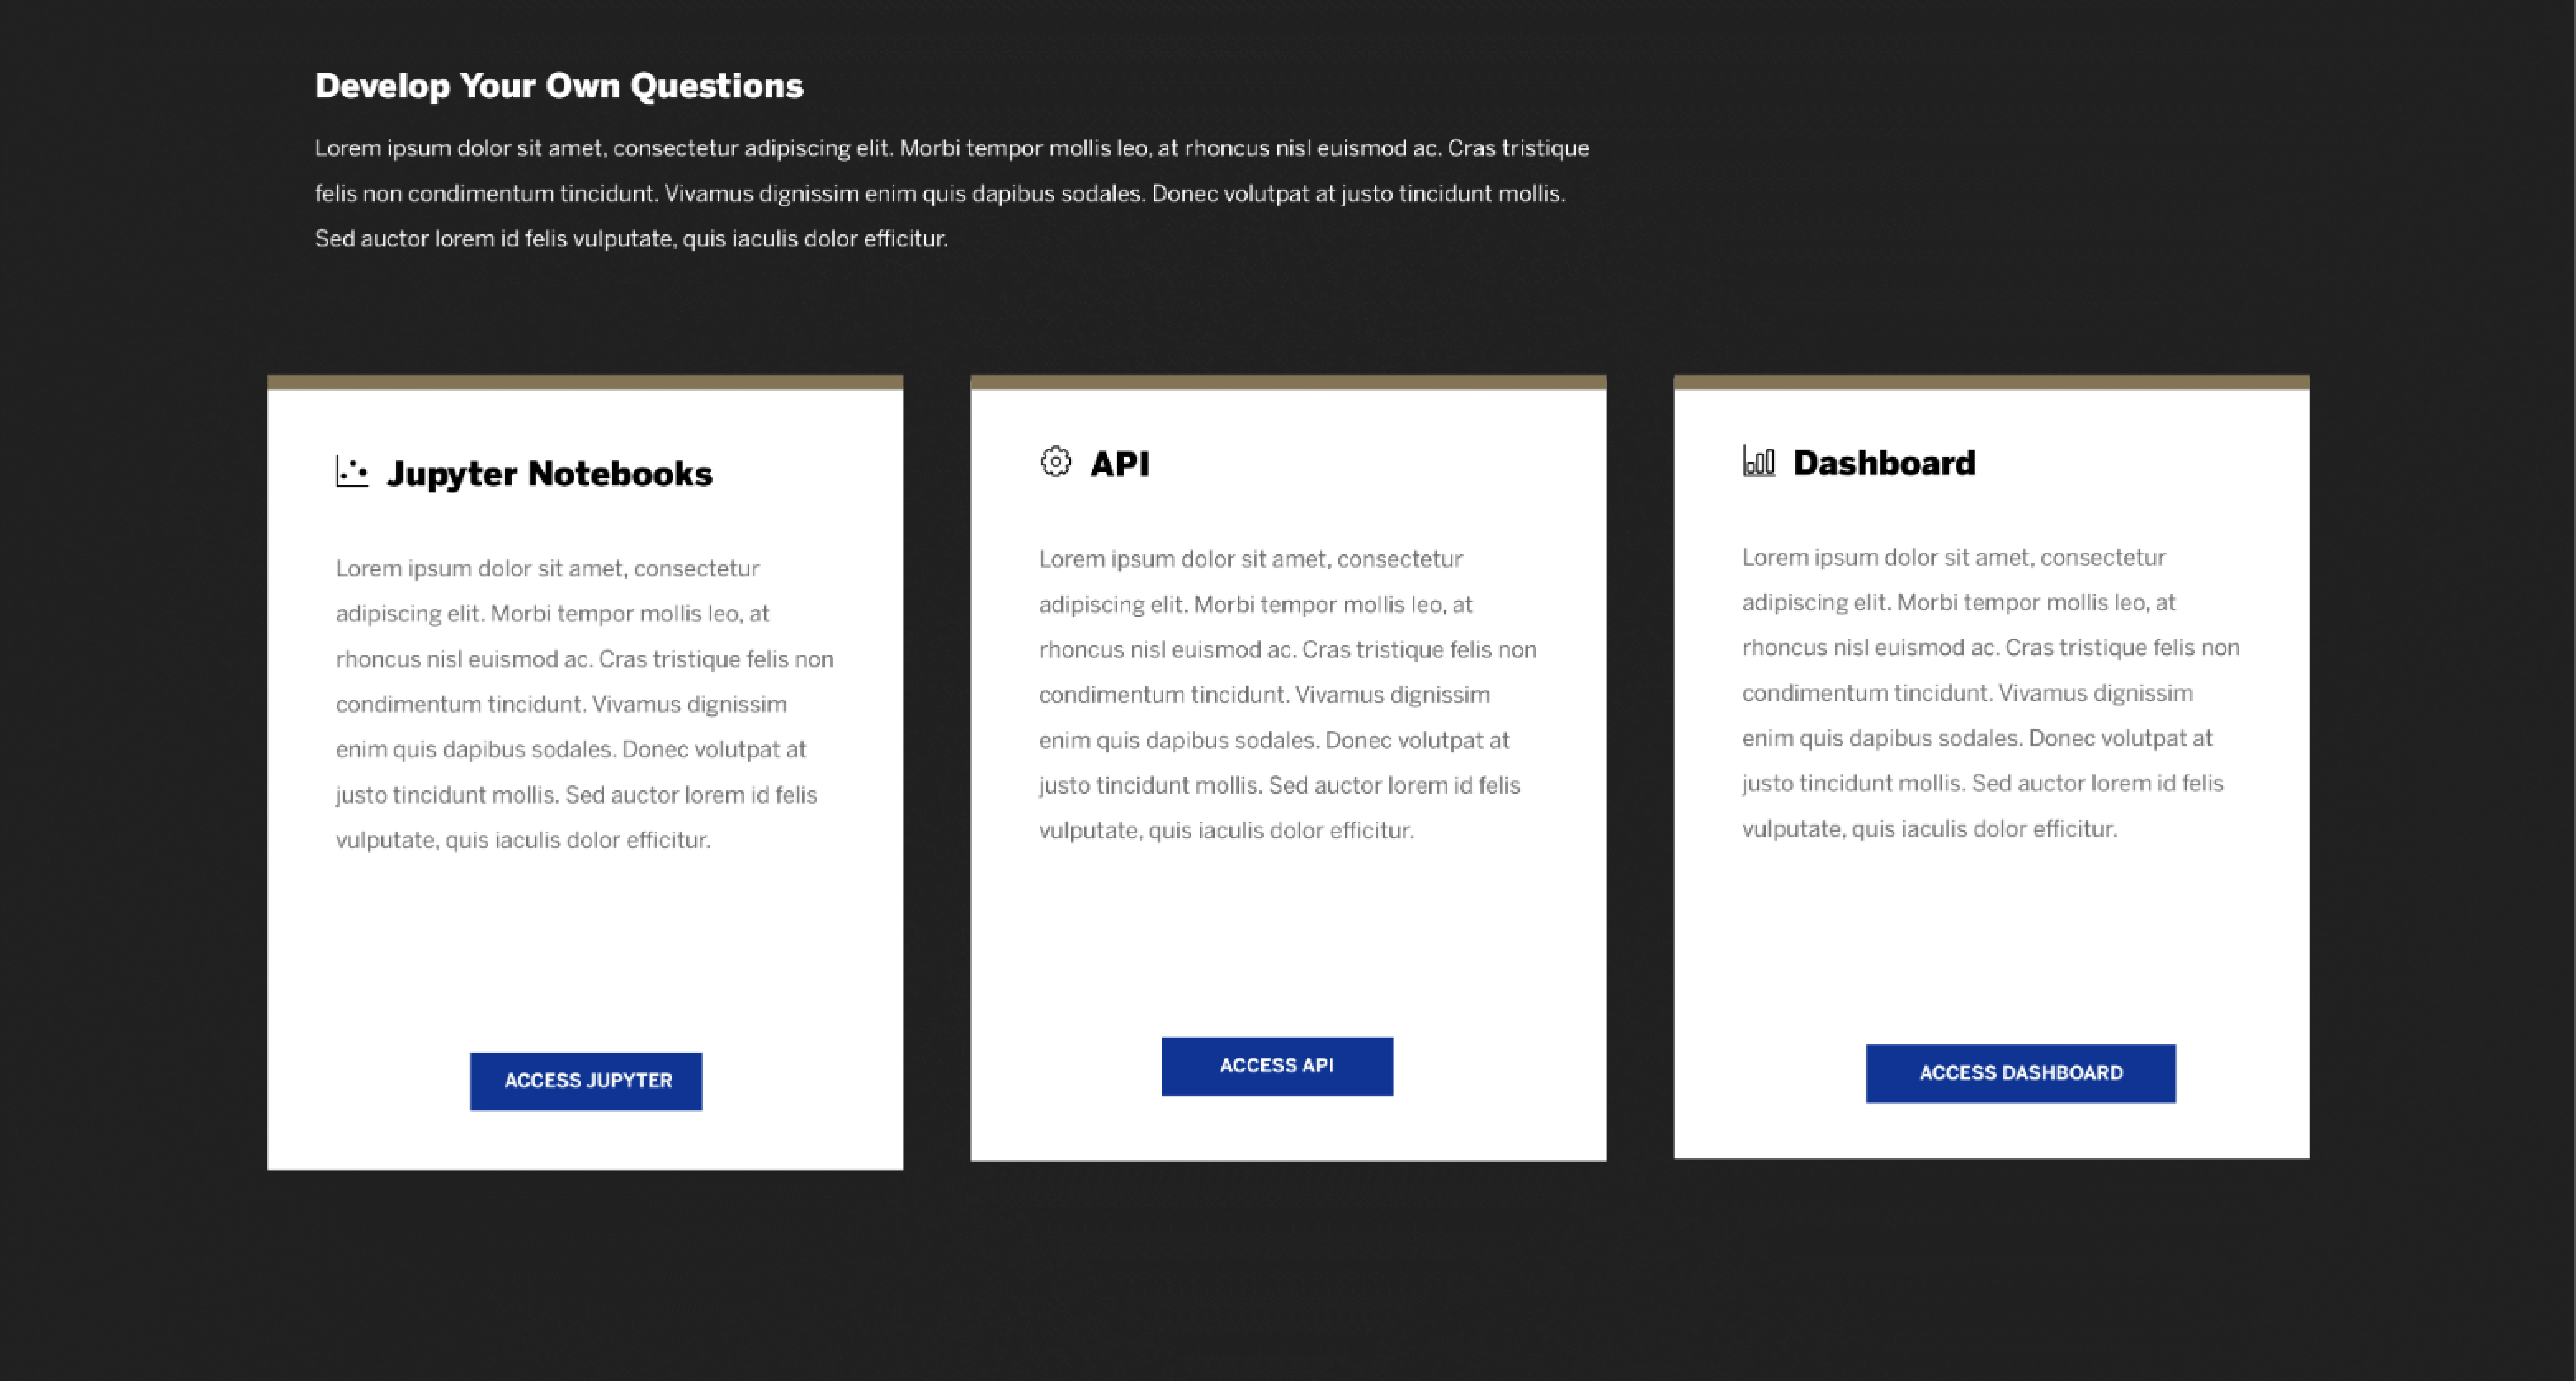
\includegraphics[scale=0.30]{user_engagement.png}
  \caption{User engagement}
  \label{fig:user_engagement}
\end{figure}
 
Initially the engagement mechanism will be workshops and webinars.  However, it is expected that the platform will include substantial modalities that allow for human-computer interaction and error correction .


\subsection{Input on User Tools}
The initial “ask” will be to get internal staff and researchers to comment on the user tools, their functionality, and the usage measures through staff briefings using the provided tools – the Jupyter Notebooks, the API and the usage/researcher dashboard – as well as develop their own questions.


Initially, these will be small workshops focused on training, exploring the platform, and collecting user experience data. During these early workshops, usability testing will also be taking place to inform and improve the tool set.

\subsection{Measures Based on a Theory of Change}
Agencies have identified a framework that they would like tested with their internal and external communities.

\newpage
% ------------------------------------ APPENDICES BELOW -----------------------------------------------------
\newpage
\section*{APPENDIX A:  METADATA SCHEMA}
  \addcontentsline{toc}{section}{APPENDIX A: METADATA SCHEMA}
\label{sec:APPENDIXA}
This describes the metadata schema. The Data Dictionary is provided in Appendix

\begin{figure}[h!]
  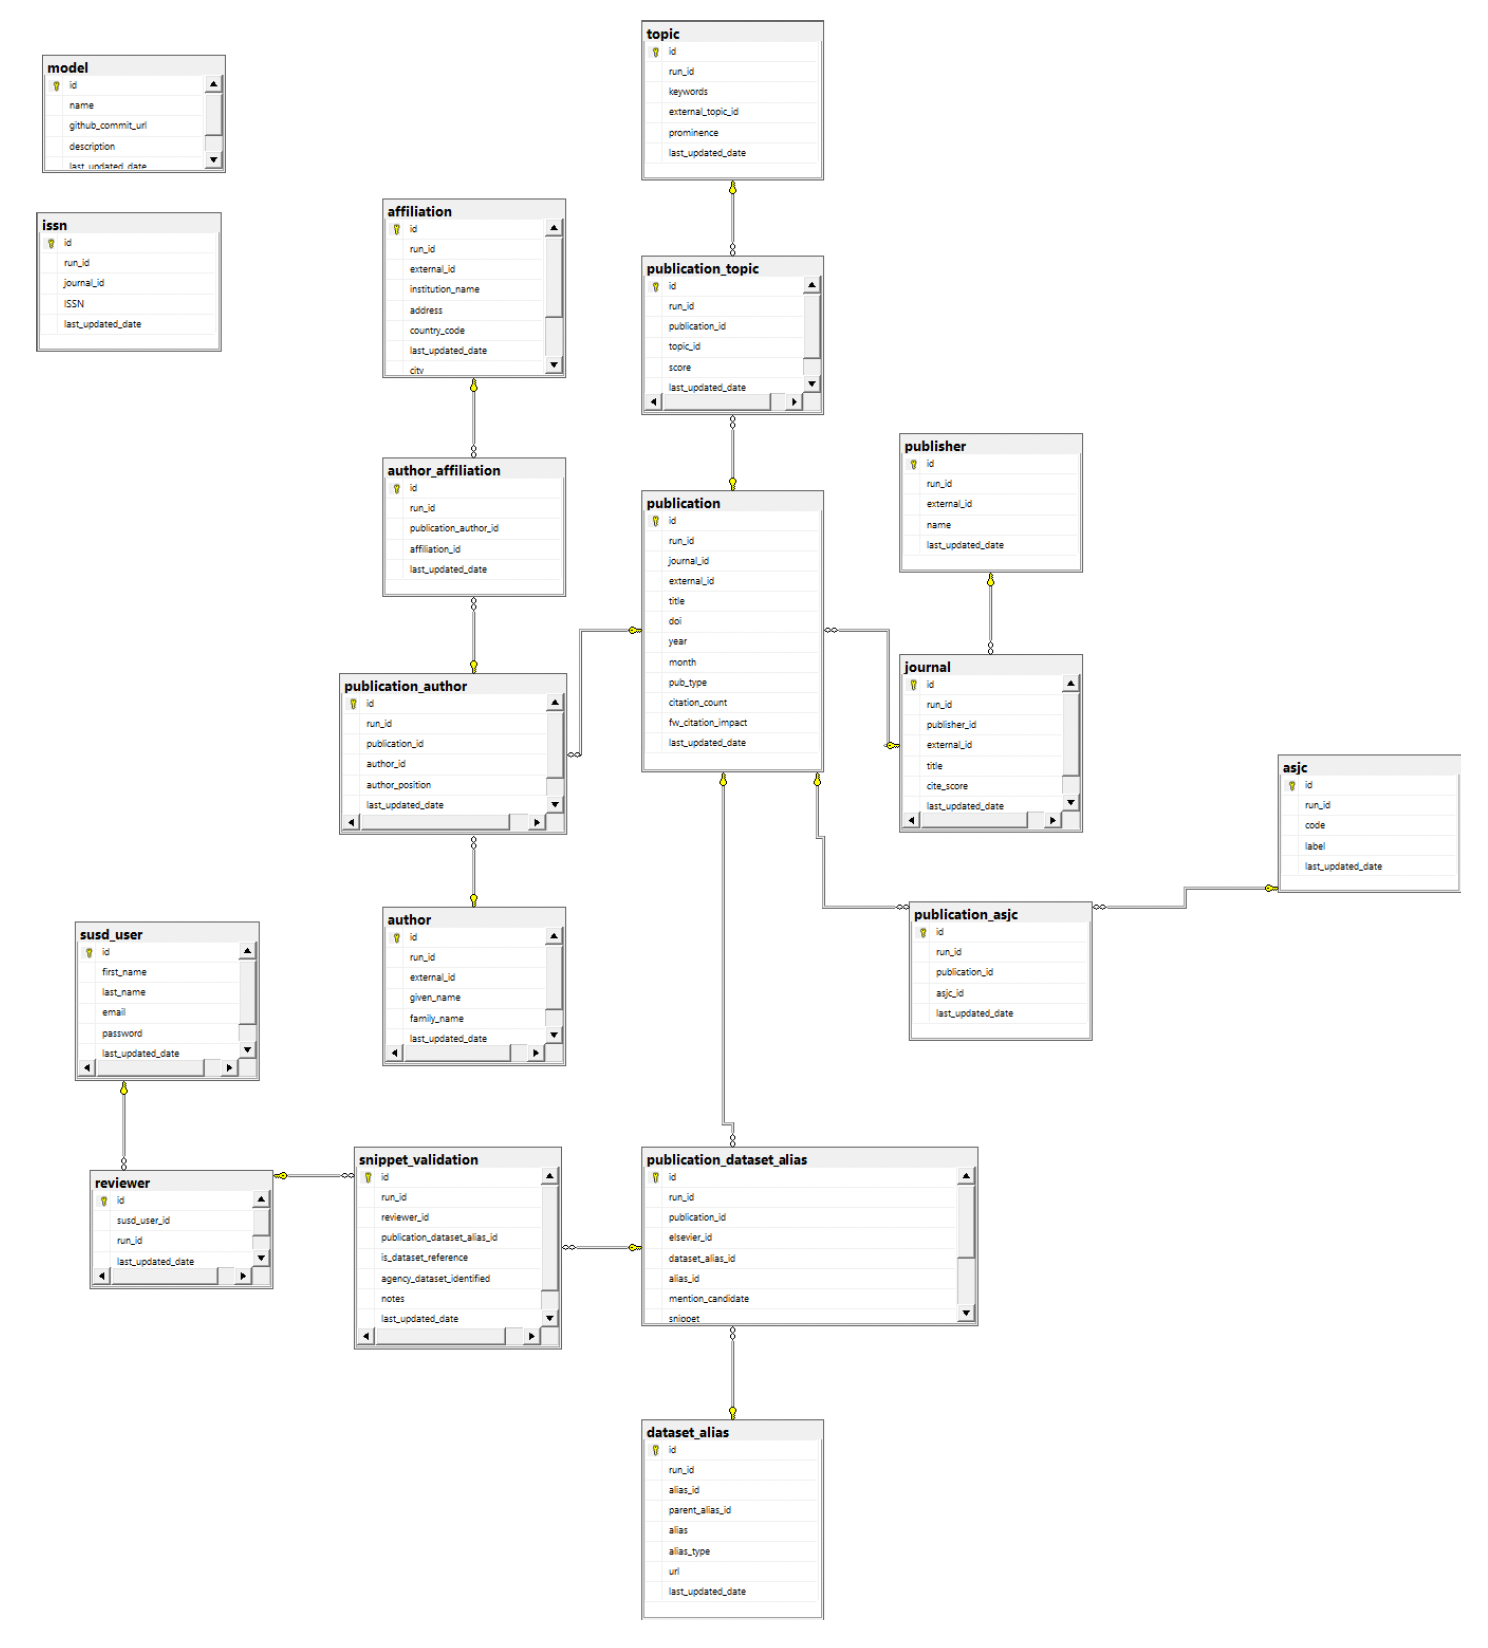
\includegraphics[scale=0.60]{AppendixA.png}
  \label{fig:appendixA}
\end{figure}

\newpage

\section*{APPENDIX B: METADATA TABLE AND DATA DICTIONARY}
  \addcontentsline{toc}{section}{APPENDIX B: METADATA TABLE AND DATA DICTIONARY}
\label{sec:APPENDIXB}

\begin{table}[h!]

{\renewcommand{\arraystretch}{1.5}%
\begin{tabularx}{1\textwidth} { 
  | >{\raggedright\arraybackslash}X 
  | >{\raggedright\arraybackslash}X 
  | >{\raggedright\arraybackslash}X 
  | >{\raggedright\arraybackslash}X
  | >{\raggedright\arraybackslash}X|}
 \hline
 \multicolumn{5}{|c|}{\textbf{AffiliationGeo : Geo information about affiliations}}\\
 \hline
 \textbf{Column name} & \textbf{Description} & \textbf{Data type} & \textbf{Length} & \textbf{Is nullable} \\
 \hline
 affiliation\_id & Nan & bigint & 0 & YES \\
 \hline
 q\_in & Nan & varchar & -1 & YES \\
 \hline
 q\_final & Nan & varchar & -1 & YES \\
 \hline
 nattempt & Nan & smallint & 0 & YES \\
 \hline
 boundingbox & Nan & varchar & -1 & YES \\
 \hline
 lat & Nan & float & 0 & YES \\
 \hline
 lon & Nan & float & 0 & YES \\
 \hline
 display\_name & Nan & varchar & -1 & YES \\
 \hline
 importance & Nan & float & 0 & YES \\
 \hline

\end{tabularx}
\label{table: appendix b - affiliation Geo}
}
\end{table}

\begin{table}[h!]

{\renewcommand{\arraystretch}{1.5}%
\begin{tabularx}{1\textwidth} {|p{3cm}|p{5.33cm}|p{2cm}|p{2cm}|p{2cm}|}
 \hline
 \multicolumn{5}{|c|}{\textbf{agency\_run: The table with runs for the different agencies}}\\
 \hline
 \textbf{Column name} & \textbf{Description} & \textbf{Data type} & \textbf{Length} & \textbf{Is nullable} \\
 \hline
 id & unique identifier to the agency\_run table & bigint & 0 & NO \\
 \hline
 agency & name of the agency for which the run was performed & varchar & 32 & NO \\
 \hline
 version & version of the run for the agency. allows multiple versions on the same data sets, or possibly new runs for the same agency but with different input data sets. & varchar & 32 & NO \\
 \hline
 run\_date & approximate date the run was performed. & date & 0 & YES \\
 \hline
 last\_updated\_date & last time the row was updated. generally the time of creation of the row. & datetime & 0 & NO \\
 \hline

\end{tabularx}
\label{table: appendix b - agency run}
}
\end{table}

\begin{table}[h!]

{\renewcommand{\arraystretch}{1.5}%
\begin{tabularx}{1\textwidth}{|p{3cm}|p{5.33cm}|p{2cm}|p{2cm}|p{2cm}|}
 \hline
 \multicolumn{5}{|c|}{\textbf{asjc: All Science Journal Classification code defines the research area of a journal and }}\\
\multicolumn{5}{|c|}{\textbf{the articles it contains.}}\\

 
 \hline
 \textbf{Column name} & \textbf{Description} & \textbf{Data type} & \textbf{Length} & \textbf{Is nullable} \\
 \hline
 id  & unique identifier for this entry & bigint & 0 & NO \\
 \hline
 run\_id & identifies the agency run for which this entry was determined, foreign key to agency\_run.id & bigint & 0 & NO \\
 \hline
 code & The All Science Journal Classification code which defines the research area of a journal and the articles it contains. There may be more than one ASJC code for each journal / publication. The 334 codes are used here providing a relatively precise definition of research area. & bigint & 0 & NO \\
 \hline
 label & TBD & nvarchar & -1 & YES \\
 \hline
 last\_updated\_date & last time the row was updated. generally the time of creation of the row. & datetime & 0 & NO \\
 \hline

\end{tabularx}
\label{table: appendix b - asjc}
}
\end{table}
\begin{table}[h!]

{\renewcommand{\arraystretch}{1.5}%
\begin{tabularx}{1\textwidth} {|p{3cm}|p{5.33cm}|p{2cm}|p{2cm}|p{2cm}|}
 \hline
 \multicolumn{5}{|c|}{\textbf{author: table with author information}}\\
 \hline
 \textbf{Column name} & \textbf{Description} & \textbf{Data type} & \textbf{Length} & \textbf{Is nullable} \\
 \hline
 id & unique identifier for this entry & bigint   & 0   & NO  \\
 \hline
 run\_id & identifies the agency run for which this entry was determined, foreign key to agency\_run.id & bigint  & 0  & NO  \\
 \hline
 external\_id & id assigned by Elsevier to the author. allow different authors to be identified across publications, even if they have different names there. & varchar & 128 & YES \\
 \hline
 given\_name  & the unique given name of the author as determined by Elsevier & nvarchar & 150 & YES \\
 \hline
 family\_name & the unique family name of the author as determined by Elsevier & nvarchar & 150 & YES \\
 \hline
 last\_updated\_date & last time the row was updated. generally the time of creation of the row. & datetime & 0 & NO\\
\hline
\end{tabularx}
\label{table: appendix b - author}
}
\end{table}

\begin{table}[h!]

{\renewcommand{\arraystretch}{1.5}%
\begin{tabularx}{1\textwidth} {|p{4cm}|p{5.33cm}|p{2cm}|p{1.5cm}|p{1.5cm}|}
 \hline
 \multicolumn{5}{|c|}{\textbf{author\_affiliation: table linking authors to their affiliations in a publication}}\\
 \hline
 \textbf{Column name} & \textbf{Description} & \textbf{Data type} & \textbf{Length} & \textbf{Is nullable} \\
 \hline
 Id & unique identifier for this entry & bigint & 0 & NO  \\
 \hline
 run\_id & identifies the agency run for which this entry was determined, foreign key to agency\_run.id & bigint & 0 & NO  \\
 \hline
 publication\_author\_id & identifies the publication\_author here linked to publication affiliation & bigint & 0 & YES \\
 \hline
 publication\_affiliation\_id & identifies the publicaiton\_affiliation entry here linked to a publication author. & bigint & 0 & YES \\
 \hline
 last\_updated\_date & last time the row was updated. generally the time of creation of the row. & date  & 0 & NO  \\
\hline

\end{tabularx}
\label{table: appendix b - author affiliation}
}
\end{table}

\begin{table}[h!]

{\renewcommand{\arraystretch}{1.5}%
\begin{tabularx}{1\textwidth} {|p{4cm}|p{5.33cm}|p{2cm}|p{1.5cm}|p{1.5cm}|}
 \hline
 \multicolumn{5}{|c|}{\textbf{dataset\_alias: Datasets provided by an agency  for a particular run and possible aliases}}\\
 \hline
 \textbf{Column name} & \textbf{Description} & \textbf{Data type} & \textbf{Length} & \textbf{Is nullable} \\
 \hline
 id & unique identifier for this entry  & bigint  & 0   & NO  \\
 \hline
 run\_id  & identifies the agency run for which this entry was determined, foreign key to agency\_run.id   & bigint   & 0   & NO  \\
 \hline
 alias\_id & the alias\_id as provided by Elsevier. & bigint  & 0   & NO  \\
 \hline
 parent\_alias\_id  & identifies the parent dataset entry in this table, as identified by the alias\_id!  & bigint   & 0   & YES \\
 \hline
 alias & the name of the data set or the alias depending on whether alias\_id==parent\_alias\_id or not. & varchar  & 160 & YES \\
 \hline
 alias\_type & flaf indicating whether the row stores the dataset itself, or an alias. & varchar  & 50  & YES \\
 \hline
 url  & URL to information about the dataset   & varchar & 2048 & YES \\
 \hline
 last\_updated\_date & last time the row was updated. generally the time of creation of the row. & datetime & 0   & NO \\
\hline

\end{tabularx}
\label{table: appendix b - dataset alias}
}
\end{table}

\begin{table}[h!]

{\renewcommand{\arraystretch}{1.2}%
\begin{tabularx}{1\textwidth} {|p{3cm}|p{6.33cm}|p{2cm}|p{1.5cm}|p{1.5cm}|}
 \hline
 \multicolumn{5}{|c|}{\textbf{dyad: The core table with dyads representing dataset references.}}\\
 \hline
 \textbf{Column name} & \textbf{Description} & \textbf{Data type} & \textbf{Length} & \textbf{Is nullable} \\
 \hline
 id & unique identifier for this entry & bigint & 0 & NO \\
 \hline
 run\_id &
  identifies the agency run for which this entry was determined, foreign key to agency\_run.id &
  bigint &
  0 &
  NO \\
  \hline
 publication\_id &
  foreign key the publication table's id column, identifying the publication within which the dataset reference represented by this dyad was identified. &
  bigint &
  0 &
  NO \\
  \hline
  elsevier\_id &
  REMOVE &
  int &
  0 &
  NO \\
  \hline
  dataset\_alias\_id &
  foreign key to the dataset\_alias table's id column identifying the match made between this dyad and a dataset alias provided by an agency. if no such match was found this column has a NULL &
  bigint &
  0 &
  YES \\
  \hline
 alias\_id &
  the intrinsic id assigned by Elsevier to the dataset alias, corresponding to the alias\_id column in the dataset\_alias table. &
  bigint &
  0 &
  YES \\
  \hline
  mention\_candidate &
  the phrase in the publication that was deemed by the algorithm to reflect a reference to a dataset &
  varchar &
  1028 &
  NO \\
  \hline
  snippet &
  snippet of text surrounding the mention\_candidate, meant to provide contextual information to reviewers/validators &
  varchar &
  -1 &
  YES \\
  \hline
  last\_updated\_date &
  last time the row was updated. generally the time of creation of the row. &
  datetime &
  0 &
  NO \\
  \hline
 is\_fuzzy &
  column has value 1 if the matching between mention candidate and dataset alias was performed using a fuzuuy algorithm, 0 otherwise. &
  bit &
  0 &
  YES \\
\hline
fuzzy\_score & 
in case the matching between mention candidate and dataset alias was perfomed using a fuzzy algorithm, this column stores the score indicating how certain the match was deemed to be. &
real &
0 &
YES \\
\hline

\end{tabularx}
\label{table: appendix b - dyads}
}
\end{table}

\begin{table}[h!]

{\renewcommand{\arraystretch}{1.5}%
\begin{tabularx}{1\textwidth} {|p{4cm}|p{5.33cm}|p{2cm}|p{1.5cm}|p{1.5cm}|}
 \hline
 \multicolumn{5}{|c|}{\textbf{dyad\_model: model scores for particular entries in the dyad table}}\\
 \hline
 \textbf{Column name} & \textbf{Description} & \textbf{Data type} & \textbf{Length} & \textbf{Is nullable} \\
 \hline
 id & unique identifier for this entry & bigint & 0 & NO \\
 \hline
 run\_id & identifies the agency run for which this entry was determined, foreign key to agency\_run.id & bigint   & 0 & NO \\
 \hline
 dyad\_id  & identifies the dyad & bigint & 0 & NO  \\
 \hline
 model\_id & identifies the model & bigint & 0 & NO  \\
 \hline
 score  & the score of this model for the dyad & real   & 0 & YES \\
 \hline
last\_updated\_date & last time the row was updated. generally the time of creation of the row.  & datetime & 0 & NO \\
\hline

\end{tabularx}
\label{table: appendix b - dyads models}
}
\end{table}

\begin{table}[h!]

{\renewcommand{\arraystretch}{1.5}%
\begin{tabularx}{1\textwidth} {|p{4cm}|p{5.33cm}|p{2cm}|p{1.5cm}|p{1.5cm}|}
 \hline
 \multicolumn{5}{|c|}{\textbf{issn: The ISSN / ISBN codes for the journal.}}\\
 \hline
 \textbf{Column name} & \textbf{Description} & \textbf{Data type} & \textbf{Length} & \textbf{Is nullable} \\
 \hline
 id & unique identifier for this entry & bigint   & 0  & NO  \\
 \hline
 run\_id & identifies the agency run for which this entry was determined, foreign key to agency\_run.id & bigint & 0 & NO \\
 \hline
 journal\_id  & foreign key to the journal table's id column, identifying the journal for this ISSN & bigint   & 0  & YES \\
\hline
ISSN & The ISSN / ISBN codes for the referenced journal/source & varchar  & 13 & YES \\
\hline
last\_updated\_date & last time the row was updated. generally the time of creation of the row. & datetime & 0  & NO \\
\hline

\end{tabularx}
\label{table: appendix b - issn}
}
\end{table}

\begin{table}[h!]

{\renewcommand{\arraystretch}{1.5}%
\begin{tabularx}{1\textwidth} {|p{4cm}|p{5.33cm}|p{2cm}|p{1.5cm}|p{1.5cm}|}
 \hline
 \multicolumn{5}{|c|}{\textbf{journal: Journal that a publication in the publication table appeared in.}}\\
 \hline
 \textbf{Column name} & \textbf{Description} & \textbf{Data type} & \textbf{Length} & \textbf{Is nullable} \\
 \hline
 id & Unique identifier and primary key for this table. & bigint   & 0    & NO  \\
 \hline
 run\_id & foreign key, identifier of the agency run for which this entry was determined. & bigint   & 0    & NO  \\
 \hline
 publisher\_id & foreign key to the publisher table, identifying the publisher for this journal at the time the agency run was executed. & bigint  & 0 & YES \\
 \hline
 external\_id & The Scopus ID for the journal / source & varchar  & 128  & YES \\
 \hline
 title & The name of the journal / source that the publication was published in.        & varchar  & 1028 & NO  \\
\hline
cite\_score   & Citescore is an Elsevier derived metric that measures the relative standing of a journal. & decimal & 0 & YES \\
\hline
last\_updated\_date & last time the row was updated. generally the time of creation of the row. & datetime & 0  & NO \\
\hline

\end{tabularx}
\label{table: appendix b - journal}
}
\end{table}

\begin{table}[h!]

{\renewcommand{\arraystretch}{1.5}%
\begin{tabularx}{1\textwidth} {|p{4cm}|p{5.33cm}|p{2cm}|p{1.5cm}|p{1.5cm}|}
 \hline
 \multicolumn{5}{|c|}{\textbf{model: The Kaggle models that are run. }}\\
 \hline
 \textbf{Column name} & \textbf{Description} & \textbf{Data type} & \textbf{Length} & \textbf{Is nullable} \\
 \hline
 id & unique identifier for this entry & bigint   & 0  & NO  \\
 \hline
 name  & the name of the model & varchar  & 32 & NO  \\
 \hline
 github\_commit\_url & the github url where the commit for this model can be found & varchar  & 1024 & YES \\
 \hline
description & description of the model  & nvarchar & -1 & YES \\
\hline
last\_updated\_date & last time the row was updated. generally the time of creation of the row. & datetime & 0 & NO  \\
\hline

\end{tabularx}
\label{table: appendix b - model}
}
\end{table}

\begin{table}[h!]

{\renewcommand{\arraystretch}{1.5}%
\begin{tabularx}{1\textwidth} {|p{3cm}|p{6.33cm}|p{2cm}|p{1.5cm}|p{1.5cm}|}
 \hline
 \multicolumn{5}{|c|}{\textbf{publication: publications discovered in a run}}\\
 \hline
 \textbf{Column name} & \textbf{Description} & \textbf{Data type} & \textbf{Length} & \textbf{Is nullable} \\
 \hline
 id & unique identifier for this entry & bigint  & 0   & NO  \\
 \hline
 run\_id & identifies the agency run for which this entry was determined, foreign key to agency\_run.id & bigint  & 0   & NO  \\
 \hline
 journal\_id & foreign key to the journal for this publicaiton& bigint  & 0   & YES \\
 \hline
 external\_id & the scopus ID (for Elsevier publications) of this publication. & varchar & 128 & YES \\
 \hline
 title & title of the publication & varchar & 400 & YES \\
 \hline
 doi  & DOI of the publication & varchar & 80  & YES \\
 \hline
 year & The year that the publication was published as recorded in Scopus & int & 0   & YES \\
 \hline
 month & The month of publication. May not be available. This will be an integer value i.e. 1 = January etc & int     & 0   & YES \\
 \hline
 pub\_type & The type of publication. Types includes - Article, review, book, book chapter, letter.  & varchar & 30  & YES \\
 \hline
 citation\_count & The number of times this publication is cited in Scopus & int     & 0   & YES \\
 \hline
 fw\_citation\_impact & The Field Weighted Citation Impact (FWCI) for the publication. This is a measure for how impactful or important a publication is as measured through normalised citations. The number of times cited divided by the expected number of citations of articles in the same year, subject and publication type. World average across papers is 1.0 for this metric. This metric also changes over time. & float & 0 & YES \\
\hline
last\_updated\_date & last time the row was updated. generally the time of creation of the row. & datetime & 0 & NO \\
\hline

\end{tabularx}
\label{table: appendix b - publication}
}
\end{table}

\begin{table}[h!]

{\renewcommand{\arraystretch}{1.5}%
\begin{tabularx}{1\textwidth} {|p{4cm}|p{5.33cm}|p{2cm}|p{1.5cm}|p{1.5cm}|}
 \hline
 \multicolumn{5}{|c|}{\textbf{publication\_affiliation: The table with affiliations on a publication.}}\\
 \hline
 \textbf{Column name} & \textbf{Description} & \textbf{Data type} & \textbf{Length} & \textbf{Is nullable} \\
 \hline
 id & unique identifier of the affiliation table & bigint   & 0   & NO  \\
 \hline
 run\_id  & identifies the agency run for which this entry was determined, 
 foreign key to agency\_run.id & bigint   & 0  & NO  \\
 \hline
 external\_id & id assigned by Elsevier to this affiliation & varchar  & 128 & YES \\
 \hline
institution\_name & the name of the institution to which a author was associated. & nvarchar & 750 & YES \\
\hline
address & the address of the author, most likely that of their institution & nvarchar & 750 & YES \\
\hline
country\_code & the three letter country code associated to the affiliaiton, most likely of the institution  & nvarchar & 10 & YES \\
\hline
last\_updated\_date & last time the row was updated. generally the time of creation of the row.& datetime & 0  & NO  \\
\hline
city & the city for the addres or institute in this affiliation   & nvarchar & 128 & YES \\
\hline
state & if appropriate, the state for the addres or institute in this affiliation & nvarchar & 128 & YES \\
\hline
postal\_code & if appropriate, the postal code for this affiliation & nvarchar & 64  & YES \\
\hline

\end{tabularx}
\label{table: appendix b - publication affiliation}
}
\end{table}

\begin{table}[h!]

{\renewcommand{\arraystretch}{1.5}%
\begin{tabularx}{1\textwidth} {|p{4cm}|p{5.33cm}|p{2cm}|p{1.5cm}|p{1.5cm}|}
 \hline
 \multicolumn{5}{|c|}{\textbf{publication\_asjc: Associative table linking a publication to ASJC entries.}}\\
 \hline
 \textbf{Column name} & \textbf{Description} & \textbf{Data type} & \textbf{Length} & \textbf{Is nullable} \\
 \hline
 id & unique identifier for this entry & bigint & 0 & NO \\
 \hline
 run\_id & identifies the agency run for which this entry was determined, foreign key to agency\_run.id & bigint   & 0 & NO \\
 \hline
 publication\_id     & foreign key to publication table's id column, identifying the publication in this relation   & bigint   & 0 & NO \\
\hline
 asjc\_id & foreign key toi the ASJC   & bigint & 0 & NO \\
 \hline
last\_updated\_date & last time the row was updated. generally the time of creation of the row. & datetime & 0 & NO \\
\hline

\end{tabularx}
\label{table: appendix b - publication asjc}
}
\end{table}

\begin{table}[h!]

{\renewcommand{\arraystretch}{1.5}%
\begin{tabularx}{1\textwidth} {|p{4cm}|p{5.33cm}|p{2cm}|p{1.5cm}|p{1.5cm}|}
 \hline
 \multicolumn{5}{|c|}{\textbf{publication\_author: Associative table linking publication and author tables.}}\\
 \hline
 \textbf{Column name} & \textbf{Description} & \textbf{Data type} & \textbf{Length} & \textbf{Is nullable} \\
 \hline
 id & unique identifier for this entry & bigint & 0 & NO \\
 \hline
 run\_id & identifies the agency run for which this entry was determined, foreign key to agency\_run.id & bigint   & 0 & NO  \\
 \hline
 publication\_id & foreign key to the publication for this author & bigint & 0 & NO \\
 \hline
 author\_id & foreigj key to the table with scopus author entries & bigint & 0 & NO \\
 \hline
 author\_position  & position of author in the list of authors on the publication  & int & 0 & YES \\
 \hline
last\_updated\_date & last time the row was updated. generally the time of creation of the row. & datetime & 0 & NO \\
\hline

\end{tabularx}
\label{table: appendix b - publication author}
}
\end{table}

\begin{table}[h!]

{\renewcommand{\arraystretch}{1.5}%
\begin{tabularx}{1\textwidth} {|p{4cm}|p{5.33cm}|p{2cm}|p{1.5cm}|p{1.5cm}|}
 \hline
 \multicolumn{5}{|c|}{\textbf{publication\_topic: identifying the topic assigned to a publication}}\\
 \hline
 \textbf{Column name} & \textbf{Description} & \textbf{Data type} & \textbf{Length} & \textbf{Is nullable} \\
 \hline
 id & unique identifier for this entry & bigint   & 0 & NO  \\
 \hline
 run\_id & identifies the agency run for which this entry was determined, foreign key to agency\_run.id & bigint   & 0 & NO  \\
 \hline
 publication\_id & foreign key to the topic table's id column identifying the publication in this relation between publications and topics. & bigint & 0 & NO \\
 \hline
topic\_id  & foreign key to the topic table's id column identifying the topic in this relation between publications and topics.  & bigint & 0 & NO \\
 \hline
 score  & TBD & real     & 0 & YES \\
 \hline
 last\_updated\_date & last time the row was updated. generally the time of creation of the row. & datetime & 0 & NO \\
\hline

\end{tabularx}
\label{table: appendix b - publication topic}
}
\end{table}

\begin{table}[h!]

{\renewcommand{\arraystretch}{1.5}%
\begin{tabularx}{1\textwidth} {|p{4cm}|p{5.33cm}|p{2cm}|p{1.5cm}|p{1.5cm}|}
 \hline
 \multicolumn{5}{|c|}{\textbf{publisher: Publishers of the journals the publications were published in.}}\\
 \hline
 \textbf{Column name} & \textbf{Description} & \textbf{Data type} & \textbf{Length} & \textbf{Is nullable} \\
 \hline
 id & unique identifier for this entry & bigint   & 0   & NO  \\
 \hline
 run\_id & identifies the agency run for which this entry was determined, foreign key to agency\_run.id & bigint   & 0   & NO  \\
 \hline
 external\_id & external identifier of this publisher in elseviers scopus repository & nvarchar & 128 & YES \\
 \hline
 name & name of the publisher  & nvarchar & 120 & YES \\
 \hline
 last\_updated\_date & last time the row was updated. generally the time of creation of the row.  & datetime & 0   & NO \\
\hline

\end{tabularx}
\label{table: appendix b - publisher}
}
\end{table}


\begin{table}[h!]

{\renewcommand{\arraystretch}{1.5}%
\begin{tabularx}{1\textwidth} {|p{4cm}|p{5.33cm}|p{2cm}|p{1.5cm}|p{1.5cm}|}
 \hline
 \multicolumn{5}{|c|}{\textbf{reviewer: Reviewers are  assigned to validate dyads in the publication\_dataset\_alias table.}}\\
 \hline
 \textbf{Column name} & \textbf{Description} & \textbf{Data type} & \textbf{Length} & \textbf{Is nullable} \\
 \hline
 id & unique identifier for this entry & bigint   & 0 & NO \\
 \hline
 susd\_user\_id & foreign key to the susd\_user table's id columns, identifying the user corresponding to this reviewer & bigint & 0 & NO \\
 \hline
 run\_id & identifies the agency run for which this entry was determined, foreign key to agency\_run.id & bigint   & 0 & NO \\
 \hline
last\_updated\_date & last time the row was updated. generally the time of creation of the row. & datetime & 0 & NO \\
\hline

\end{tabularx}
\label{table: appendix b - reviewer}
}
\end{table}

\begin{table}[h!]

{\renewcommand{\arraystretch}{1.5}%
\begin{tabularx}{1\textwidth} {|p{4.3cm}|p{5.33cm}|p{2cm}|p{1.2cm}|p{1.5cm}|}
 \hline
 \multicolumn{5}{|c|}{\textbf{snippet\_validation: the validation results for dyads provided by reviewers}}\\
 \hline
 \textbf{Column name} & \textbf{Description} & \textbf{Data type} & \textbf{Length} & \textbf{Is nullable} \\
 \hline
 id & unique identifier for this entry & bigint   & 0  & NO  \\
 \hline
 run\_id  & identifies the agency run for which this entry was determined, foreign key to agency\_run.id  & bigint   & 0  & NO  \\
 \hline
 reviewer\_id & foreign key to the reviewer table's id column, identifying the reviewer assigned to validate this snippet & bigint   & 0  & NO  \\
 \hline
 dyad\_id & foreign key to the dyad table's id column, identifying the dyad that is being validated. & bigint   & 0  & NO  \\
 \hline
 is\_dataset\_reference & if the value in this column is 1 it indcates the dyad indeed has identified a reference to a datasdet, if 0 it is not a dataset reference, if -1 the reviewer was unsure about it. & smallint &
  0 & YES \\
  \hline
 agency\_dataset\_identified & if the value in this column is 1 it indicates the dyad indeed identified the specific dataset provided by the agency, if 0 it is not a reference to that dataset, if -1 the reviewer was unsure about it. & smallint & 0 & YES \\
 \hline
 notes & any notes the reviewer attached to the dyad being reviewed & nvarchar & -1 & YES \\
 \hline
 last\_updated\_date & last time the row was updated. generally the time of creation of the row. & datetime & 0  & NO \\
\hline

\end{tabularx}
\label{table: appendix b - snippet validation}
}
\end{table}

\begin{table}[h!]

{\renewcommand{\arraystretch}{1.5}%
\begin{tabularx}{1\textwidth} {|p{4cm}|p{5.33cm}|p{2cm}|p{1.5cm}|p{1.5cm}|}
 \hline
 \multicolumn{5}{|c|}{\textbf{susd\_user: A user of the validation tool.}}\\
 \hline
 \textbf{Column name} & \textbf{Description} & \textbf{Data type} & \textbf{Length} & \textbf{Is nullable} \\
 \hline
 id          & unique identifier of this table & bigint  & 0   & NO  \\
 \hline
first\_name & First name of the individual.   & varchar & 100 & YES \\
\hline
last\_name  & Surname of the individual.      & varchar & 100 & YES \\
\hline
email       & email of the user.              & varchar & 100 & YES \\
\hline
password    & encrypted password of the user. & varchar & 100 & YES \\
\hline
last\_updated\_date & last time the row was updated. generally the time of creation of the row. & datetime & 0 & NO \\
\hline

\end{tabularx}
\label{table: appendix b - susd user}
}
\end{table}

\begin{table}[h!]

{\renewcommand{\arraystretch}{1.5}%
\begin{tabularx}{1\textwidth} {|p{4cm}|p{5.33cm}|p{2cm}|p{1.5cm}|p{1.5cm}|}
 \hline
 \multicolumn{5}{|c|}{\textbf{topic: topics defined by Elsevier and assigned to publications. consist of three}}\\
 \multicolumn{5}{|c|}{\textbf{concatenated keywords}}\\
 \hline
 \textbf{Column name} & \textbf{Description} & \textbf{Data type} & \textbf{Length} & \textbf{Is nullable} \\
 \hline
 id  & unique identifier for this entry & bigint  & 0   & NO  \\
 \hline
 run\_id  & identifies the agency run for which this entry was determined, foreign key to agency\_run.id  & bigint  & 0    & NO  \\
 \hline
 keywords & a topic is defined in Elsevier by three keywords. This columns sotres these as a |-separated string. & varchar & 1028 & YES \\
 \hline
 external\_topic\_id & external identifier of this topic provided by Elsevier. & varchar & 128 & YES \\
\hline
prominence  & TBD  & real     & 0 & YES \\
\hline
last\_updated\_date & last time the row was updated. generally the time of creation of the row. & datetime & 0 & NO  \\
\hline
last\_updated\_date & last time the row was updated. generally the time of creation of the row. & datetime & 0 & NO  \\
\hline

\end{tabularx}
\label{table: appendix b - topic}
}
\end{table}



\clearpage
\section*{APPENDIX C: TECHNICAL WORKFLOW DESCRIPTION}
  \addcontentsline{toc}{section}{APPENDIX C: TECHNICAL WORKFLOW DESCRIPTION}
\label{sec:APPENDIXC}

\textbf{\textcolor{TealBlue}{Partners}}
\begin{description}
   \item[EL] Elsevier
   \item[IDIES] Institute for Data Intensive Engineering and Science, Johns Hopkins University
   \item[NYU] New York University
   \item[TACC] Texas Advanced Computing Center at the University of Texas at Austin
\end{description}

\bigskip

\textbf{\textcolor{TealBlue}{Roles}}
\begin{description}
    \item[SYSADMIN] a defined user of the admin dashboard who has been authorized by the Democratizing Data leadership to initialize projects that an agency has requested and to assign users as administrators of those projects
    \item[ADMIN] a defined user from the agency staff who has been assigned by the agency to manage a project, configure its input parameters, monitor progress, and assign reviewers, etc.
    \item[REVIEWER] a user assigned by the admin to review/validate the results of the machine learning algorithms.
\end{description}

\bigskip

\textbf{\textcolor{TealBlue}{Glossary/Definitions}}
\begin{description}
    \item[Project] A dataset search and discovery activity requested and defined by a funding entity (currently federal agency). It is characterized in a statement of work by a set of datasets that are targets of the inquiry, as well as a set of restrictive parameters. 
    \item[Main Alias] The main alias is the dataset name that most commonly describes the dataset and/or the dataset which the agency would wish results to be grouped by. 
    \item[Alias Type] Many Datasets have short form names or alternative names that are used instead of the Main Alias. These are dataset aliases. A specific form of alias is an acronym or abbreviation. Where such aliases exist they can form part of the search routines. 
    \item[Research Output] A document / publication representing the formal results of research. Research outputs include journal articles, conference papers, review papers, book chapters, books etc.
\end{description}

\bigskip

\textbf{\textcolor{TealBlue}{Steps}}

Indicated by a sequence number and by location

\bigskip
\bigskip

\underline{\textbf{Step 0: Project initialization [IDIES]}}

A \textbf{SYSADMIN} initializes a new project in the admin dashboard.

This requires the following actions:
\begin{enumerate}
    \item Adding project level metadata such as: \begin{itemize}
        \item Formal department name (e.g., USDA or US Department of Agriculture)
        \item Formal agency name (e.g., NASS or National Agricultural Statistical Service)
        \item Unique identifier which includes a date stamp and version number (e.g., 2022\_12\_15\_v1)
    \end{itemize}
    \item Assigning a "defined user" to be ad ADMIN for this project and communicating with that ADMIN user to explain entry to the system.
\end{enumerate}

Side effects:
\begin{itemize}
    \item An entry representing the project will be written in the \texttt{agency\_run} table.
    \item An entry representing the agency \textbf{ADMIN} will be added to the \texttt{reviewer} table.\begin{itemize}
        \item if no user exists yet an entry will also be added to the \texttt{susd\_user} table.
    \end{itemize}
    \item An entry will be added to the \texttt{agency\_run\_history} table.
\end{itemize}

\bigskip

\underline{\textbf{Step 1: Project definition [IDIES]}}

Agency ADMIN uploads target dataset-alias file format: either

\textbf{csv\footnote{Note that Excel is discouraged because it typically eliminates leading zeroes and can thus negatively affect the functionality of identifiers
}}: % note theres a citation here

\hspace{1cm}
\begin{minipage}{\textwidth}

Each row should correspond to a dataset name/alias

columns:
\begin{itemize}
    \item \texttt{Main\_alias\_id}: identifier, created by NYU upon receipt and unique in file
    \item \texttt{Main\_alias}: the string identifying name of dataset identified by the agency as the formal name of the dataset
    \item \texttt{\_alias\_name}: identifies and aliases that are commonly associated with \texttt{Main\_alias}
    \item \texttt{alias\_type}: one from [\texttt{main\_alias}, acronym]
    \item Dataset DOI: if available
    
\end{itemize}

\end{minipage}


or

\textbf{JSON}:

\hspace{1cm}
\begin{minipage}{\textwidth}

\begin{lstlisting}[language=json, firstnumber=1]
{"dataset": <dsname>,
 "aliases": [{"alias": <alias>,
              "type": <one of ["alias", "acronym"]>}
 
 ],
 ...
}
\end{lstlisting}
\end{minipage}

\textbf{ADMIN} set other search config parameters:
\begin{itemize}
    \item data range: [start-date, end-date] where data is ISO-8601 compliant (YYYY-MM-DD) and based on calendar year
    \item US author flag: boolean
\end{itemize}

\textbf{ADMIN} clicks button to save or submit:
\begin{itemize}
    \item \textbf{save}: result stored in database \begin{itemize}
        \item Data model extension needed.
        \item History of consecutive save-s stored.
    \end{itemize}
    \item \textbf{submit}: Elsevier notified \begin{itemize}
        \item TBD how: likely file uploaded to new S3 folder that \textbf{Elsevier} is listening to
        \item milestone noted in database
    \end{itemize}
\end{itemize}

\bigskip
\underline{\textbf{Step 2: Identify relevant topics for search corpus creation [EL]}}

\textbf{Elsevier} uses the job identifier created in step 0 to organize its work and undertakes process as follows: 
\begin{itemize}
    \item Take datasets names and aliases from step 1;
    \item Exact text marching on Science Direct;
    \item Identify the Research Topics on the matches generated;
    \item Aggregate the counts of matched research outputs by Topics;
    \item Apply filter that excludes those topics with less than a count of 5 research outputs.
\end{itemize}

\textbf{Elsevier} transmits a JSON file containing resulting list of Research Topics from Science Direct to \textbf{IDIES} with the following aggregate metadata:
\begin{itemize}
    \item unique run identifier;
    \item Research Topics;
    \item count of research outputs against the filtered Research Topics.
\end{itemize}

NYU and IDIES review and select the research topics with EL.

\textbf{IDIES} shows the result in the admin dashboard and stores milstones in database.

\textbf{ADMIN} inspects result (Note that in V2 agencies will be able to provide input).

\bigskip
\underline{\textbf{Step 3: Determination search corpus [Elsevier]}}

\textbf{Elsevier} determines the input for the ML Algorithms:
\begin{itemize}
    \item Search Scopus using Research Topics and the search config parameters and identify the research outputs records that are theoretically available for the search corpus. \begin{itemize}
        \item Output 2.1 Number of records theoretically available in Scopus.
    \end{itemize}
    \item Filter the records to exclude those for which full text does not exist.\begin{itemize}
        \item Output 2.2 Number of records for which full text exists.
    \end{itemize}
    \item Exclude records for which full text search is not allowed because of licensing agreements. \begin{itemize}
        \item Output 2.3 Number of records for which full text exists and we are licensed that may be searched. 
    \end{itemize}
    \item From this filtered set of research outputs, identify the Research Topics and calculate the number of research outputs that are linked to each topic.
    \item Filters topics to include only those with more than 5 research outputs per topic. 	\begin{itemize}
        \item Output 2.4: List of research topics with counts of research outputs greater than 5
    \end{itemize}
\end{itemize}

\textbf{Elsevier} transfers Outputs 2.1 to 2.4 to \textbf{IDIES} in a JSON file.

\textbf{IDIES} displays results on the dashboard and stores milestone in the database.

\textbf{ADMIN} inspects the result (Version 2 will allow more interaction).

\bigskip
\underline{\textbf{Step 4: Running ML algorithms [Elsevier]}}

\textbf{Elsevier} runs the ML models on the Search Corpus:

\begin{itemize}
    \item Record the results of the models in a way that enables the different results generated by the different models to be later compared (i.e. which datasets were found by which models).
    \item Perform fuzzy match using the alias names to determine whether the datasets found by the ML models ae on the agency dataset list and tags with the unique identifier. 
    \item Filter the set of matched records to indicate which are associated with target datasets and those where snippet cannot be generated for licensing reasons
\end{itemize}

\textbf{Elsevier} provides aggregate metadata about the run to \textbf{IDIES}.

For target dataset:
\textbf{
\begin{itemize}
    \item Dataset name;
    \item Unique ID for dataset;
    \item Flag for whether dataset is in agency search list;
    \item Name of model(s) that found the dataset;
    \item Threshold chosen for inclusion;
    \item Count of number of mentions;
    \item Count of number of unique research outputs in which that dataset has been found;
    \item Count of number of publications for each research topic.
\end{itemize}
}

For unknown datasets with frequency greater than 5:
\textbf{
\begin{itemize}
    \item Predicted name of unknown dataset;
    \item Count of number of mentions;
    \item Count of number of unique research outputs in which that dataset has been found;
    \item Count of number of research outputs for each research topic.
\end{itemize}
}

\textbf{IDIES} displays this in admin dashboard and records milestone in databases.
\textbf{ADMIN} inspects the result and approves continuation. [precise details TBD].

\bigskip
\underline{\textbf{Step 5: Generation Publication Record Data for validation [Elsevier]}}

\textbf{Elsevier} takes the research outputs that are matched with one or more target datasets and produces the agreed metadata for those research output records (see \hyperref[sec:APPENDIXB]{Appedix B} for metadata that is available for individual research outputs). The data for individual research records is for those that contain the target datasets or their aliases only. 

Whilst research output metadata is produced only for the research output that contain a target dataset or alias, it is possible that a research output will contain other datasets in addition to the target ones. In those circumstances, the snippet associated with those additional datasets will be provided.

\bigskip
\underline{\textbf{Step 6: Ingestion in database [IDIES]}}
\begin{itemize}
    \item \textbf{IDIES} retrieves data from S3 storage on SciServer;
    \item JSON files read and ingested into staging database;
    \item Data from staging tables transformed into core database;
    \item Admin dashboard shows statistsics such as: \begin{itemize}
        \item total number publications found;
        \item number of research outputs for each dataset;
        \item number of topics for each dataset show topics sorted in descending frequency;
        \item number of authors for each dataset;
        \item number of journals for each dataset.
    \end{itemize}
\end{itemize}

\bigskip
\underline{\textbf{Step 7: Validation [IDIES]}}

\textbf{ADMIN} configures validation:
\begin{itemize}
    \item defines users (email, password);
    \item assigns users as \textbf{REVIEWER} for this project;
    \item sets number of snippets in a batch;
    \item sets fraction of snippets whith multiple reviews.
\end{itemize}

\textbf{REVIEWER} validates snippets assigned to them.

\textbf{ADMIN} inspects progress of validation in admin dashboard.

V2 ADMIN provides map of EL research topics to AGENCY topic of interest.

\medskip
\underline{\textbf{Step 8: Finalization [IDIES]}}

\textbf{ADMIN} decides validation is complete.

Validated data is sent to S3 bucket.
\begin{itemize}
    \item One CSV file per table.
    \item Only accepted dyads, no snippet data
\end{itemize}

\textbf{TACC} retrieves it and loads it in database underlying the API.

\textbf{Elsevier} extracts information of use for ML tuning.

\newpage
\section*{APPENDIX D: SHOW US THE DATA WORKSHOP RESULTS}
  \addcontentsline{toc}{section}{APPENDIX D: SHOW US THE DATA WORKSHOP RESULTS}
\label{APPENDIXD}

\subsection*{Chief Data Officers and Evidence Act Officials} \label{subsec:CDOE}
On September 21, 2021, the Coleridge Initiative convened a panel of Evidence Act Officials and Chief Data Officers to request their input about the results of the “Show US the Data” competition before the October 20th workshop.  The goal of the CDO expert pre-session was to develop a point of view from representative CDOs regarding the applicability of the learnings and tools developed in the “Show US the Data” competition.   Since the competition focused on uses of data sets in research, the outcomes were most immediately appliable to agencies with scientific mission components.   CDOs from agencies for which discovery activities occurred in the competition were invited to review results in one-on-one sessions and then to attend this panel discussion.  The Agencies represented in the discussion were Commerce (NOAA), NSF, USDA, Transportation.   Given that the breadth of data work in an Agency may cross many mission teams, some agencies had multiple team members participate in the discussion session.

Specific questions were posed to identify ways that the approach and prototype algorithms might be used to support agency mission activities both near-term and strategically, including \begin{enumerate*}[label=(\arabic*)]
    \item how the capabilities might be used;
    \item opportunities for near term use in the agencies; 
    \item potential obstacles to use; 
    \item key points of engagement; 
    \item proposed next steps.
\end{enumerate*}

The type of tools developed in the competition might support emerging research themes, connect researchers to previously undiscovered datasets for stimulating new discovery, and providing evidence of citizen benefits. As such, they are more useful for prioritizing resources and work efforts for making public data available for research and public uses than as simply a pathway to achieve compliance with the Open Public Electronic Necessary Government Data Act and other mandates. They can drive broader visibility and transparency about datasets and their uses both within and outside the agencies. Most impactful would be creating communities around connecting and creating meaningful exchanges between the users of the data and those producing and maintaining the data. 

One important barrier to use is the agencies’ lack of current workforce skills for developing and using these types of technical tools.   Also discussed were competing priorities for resources within agencies and overall priorities of Agency mission activities. 

Building greater visibility and engagement would require a significantly expanded awareness outreach effort that could include Boards, special purpose groups, councils and civic tech organizations.

The discussions about near-term use and next steps coalesced into a common point – identification of specific use cases within Federal agencies to sponsor application of the approach and tools followed by analysis and capture of learnings from each step along the process-priority setting, workforce, barriers and engagement model.

It was suggested by the participants that the October session include some dialogue about potential use cases so that there might be collective sponsorship and support for the next steps. 

\subsection*{Academic Researchers}\label{subsec:AcademicResearchers}
The Coleridge Initiative convened a panel of experts representing the perspective of researchers to get their input about the results of the “Show US the Data” challenge before the October 20 conference. The goal of the panel was to gain understanding about a new machine learning approach to identifying public uses of agency data, identify strengths and weaknesses of the approach, discuss how researchers would draw on this usage information captured by live data streams, and suggest ways to incorporate feedback from the public on both the usage documentation and on the data sets.  The panel discussion will be summarized and incorporated in the October conference.

The participants were asked a series of structured questions including: \begin{enumerate*}[label=(\arabic*)]
    \item how they might use the tools to advance their research;
    \item how the tools might advance the work of junior researchers; 
    \item how the tools might inspire researchers to do their work differently; and 
    \item how might the researcher community become engaged in this effort? 
\end{enumerate*}  Below are some key highlights summarized.  Detailed minutes are attached.
\begin{itemize}
    \item Providing the right incentives for researchers facilitates success and encourages use and feedback to improve the system. The tools can assure that the burden is not all on the researcher to provide their publication data. Rather, a positive feedback loop could be created by researchers having their citations and publications included, getting people to advertise their work, giving seminars, and sharing their data and best practices in terms of citing data, so that their work can get acknowledged. This also could lead to improvements such as a uniform citation for a dataset. 
    \item The tools allow researchers to make connections between what datasets are being used and for what purposes—allowing researchers to build on what’s already been done. Making connections also highlights which datasets may be underused. The tools can also foster partnerships between academic researchers and government agencies that have data the researchers are using. Those two-way relationships can also help improve the data sets’ accuracy and usability.
\end{itemize}

\subsection*{Publishers}\label{subsec:publishers}
The Publisher workshop was held in conjunction with three other workshops (Chief Data Officers, Researchers, and Academic Institutions) to answer questions and gather input to feed into the Coleridge Initiative “Show US the Data Conference” on October 20, 2021. Structured questions were asked to get feedback on what the academic institution stakeholder community thinks about Machine Learning/Natural Language Processing. 

The workshop participants were asked structured questions to get feedback on what the publisher stakeholder community thinks about the potential of the Rich Text Content project and its machine learning and natural language processing components. \begin{enumerate*}[label=(\arabic*)]
    \item Concerns about the Machine Learning / Natural Language Processing (ML/NLP) approach to capturing data use; 
    \item Additional functionality that would be useful;
    \item the value proposition for publishers to participate;
    \item How publishers could participate; and 
    \item where should the application reside and be managed?
\end{enumerate*}

The participants raised several points including:

\begin{itemize}
    \item This initiative needs to be a sustainable infrastructure where there is funding for work that is produced, and there is value in producing a high-quality curated corpus. There should be transparency in any pricing model. The small to medium publishers have valuable content and contributions but have a lower level of sophistication which may impact the rate of adoption.
    \item There should be a central place, such as data.gov, where this information can be accessed. In addition, a publisher dashboard maintained for smaller publishers could be very helpful so that publishers could also see how data are being used, citations, and new services that publishers could provide.
    \item One of the biggest challenges with reusing and understanding the ongoing value of datasets is how much metadata is there and how much context there is around that data. Researchers are also funded in a way that they don’t have access to those government repositories and are left with fewer choices to put their data so they end up in general repositories like Figshare, Dryad, etc. General repositories aren’t very helpful for building on research unless they are able to pull in the required metadata. There is a need for greater incentive for authors to comply with open data policies.  If publishers make this more findable and prominent and enable credit as a first class object: incentives, quality, services, and compliance will increase. 
\end{itemize}

Other discussion points raised included: 

\begin{itemize}
    \item \textit{Value Proposition}: many publishers are investigating services that they might provide in relation to identification and analysis in getting data. Is this a free substitute for something that they would like to provide a service as part of a publisher’s offerings? What is the value proposition for publishers? 
    \item \textit{Bias}: Having machine learning drawing conclusions about how data are being used may not lead to the most accurate insights. How can human interaction be added into the model to improve the results and the accuracy will continue to grow.
    \item \textit{Relative importance of two main use cases}: \begin{enumerate*}[label=(\arabic*)]
        \item a compliance driven use case -- for agencies to show that they are tracking reuse per the mandate; and
        \item providing a means to discover data.
    \end{enumerate*} To what extent has the relative importance of these use cases been established with users? 
    \item \textit{Risk of using NLP to capture data}: in making our entire Full text XML corpus available to do the work, how to ensure the content was only used for this purpose, by a controlled group, and deleted afterwards. This doesn’t relate to concerns about the job itself (publishers do make content available to third parties for indexing, abstracting, etc).
    \item A link back to the publisher is critical, ultimately building an informal citation network. The community develop different visualizations to suit their needs?
    \item Publishers can participate in multiple ways, including allowing indexing services to use their  content for this purpose; or running the ML/NLP algorithms internally on their content. Harvesting is currently allowed by some publishers.
    \item A public/private partnership that would be friendly to international users and be resilient to US administrative government change could be  considered to run this function, with central access available. 
    \item A broad general value proposition is enhancing your value (both quantitatively and qualitatively) to the community you are trying to serve. There are also non-financial benefits for publishers, such as increased usage and citations. Publishers want to comply with funder goals, long term solution is more around formal citation (as mentioned earlier), and Value proposition on “win-win” content/data discovery, links between the two (more consumers of government data and more consumers of published articles) the technical and business challenges in creating a long-term solution? Could a combined effort be established?
    \item There is a need for equity across publishers and potentially there was additional enabling needed for smaller publishers. Most are doing things in a different way, so thinking in terms of using a broker where there is a degree of standardization may be a good idea.
\end{itemize}

The participants agreed that it may make sense to start off with a pilot on one or two specific topics.
\begin{itemize}
    \item The tools foster community and mentorship, helping junior researchers use data to knit together people and research to impact their work. Junior researchers could discover new data sets and ways to use existing data sets and gain visibility if their research is represented in the database. 
    \item An interactive partnership approach between agencies and the research community can help agencies prioritize by seeing how data are being used by others. Agencies can use the buy-in of researchers—documented as high use of certain datasets—to demonstrate its importance to Congress, call attention to underutilized data, and make investments in data improvement.

\end{itemize}

Several ideas were put forth to encourage researcher community engagement:

\begin{itemize}
    \item Researchers could be incentivized by providing curation tools—for example, finding related datasets by joining datasets and cleaning up the data. Agencies could provide links to tools for cleaning and linking the data. Some researchers may not know how much data are available to them from agencies. Some younger researchers find this out only by asking more senior researchers. 
    \item Access to grey literature (research that has not been published in a peer reviewed journal but are available in libraries of universities and elsewhere) could be incredibly valuable, creating communities around working papers and even avoiding publication bias. 
    \item The tools offer further opportunity for development, such as information regarding authors (name, email addresses, etc.) could be harvested or a Citation Index drawn on for collaborators, allowing authors and other researchers in the field to build up a network to share information about certain metadata and otherwise clarify uncertainties, fill gaps, and improve overall use. Researcher could automatically share information about the quality of a dataset.

\end{itemize}

The panel identified the key next actions as follows: 

\begin{itemize}
    \item The project should stay focused on the value add and allow for exciting developments.
    \item Researchers should be able to see how easy the tool is to use and immediately see the value. Engaging high profile users—research “influencers”—could also be a great way to set a trend among others. 

\end{itemize}

\subsection*{Academic Institutions}\label{subsec:Academicinstitutions}
The Academic Institutions workshop was held in conjunction with three other workshops (Chief Data Officers, Researchers, and Publishers) to answer questions and gather input to feed into the Coleridge Initiative Show US the Data Conference on October 20, 2021. Structured questions were asked to get feedback on what the academic institution stakeholder community thinks about Machine Learning/Natural Language Processing. 

The participants discussed several issues and brought up the key points below:
\begin{itemize}
    \item Several benefits for researchers at institutions included improved discovery of what data exist and are available, better access to data, and opportunities for collaboration, especially across disciplines.  More use of the data would also create motivation to improve the metadata, e.g., developing and conforming to metadata and citation standards and making sure data are complete. This would also help improve existing governance structures and help integration across existing infrastructures.
    \item Institutions want to understand usage and improve discovery and access from their data repositories. Institutions also use a lot of state and other data, so there could be wider applications beyond federal data.  The application could also help identify gaps in which data were being underutilized.  In addition, preservation policies for data could use data to support decisions, e.g., a librarian to check after a period of time to see if data has been used, and if no one has used the data, could archive it or stop maintaining it. The cumulative costs of maintaining repositories are going to be important and will be impacted by the use case of determining which datasets should be kept for what period of time. 
    \item Some land grant universities have close relationships with federal agencies such as USDA. It could be helpful to consider pilot projects that build on these relationships.

\end{itemize}

\subsection*{Miscellaneous}
Other discussion points included:
\begin{description}
    \item [Concerns.] Participants expressed a desire for data beyond those in scientific publications (“gray” literature, other media), ensuring the accuracy of data included in the dashboards, and establishing a mechanism for feedback on what agencies are doing with public comments and suggestions on improving the data.  Privacy concerns related to the ability of competing institutions and researchers to view the dataset details that an institution is using, particularly prepublication. Questions arose on who would run such a service and be responsible for protecting privacy, uncovering potential bias, and usability. 
    \item [Participation and access.] A central host was generally favored but institutions also wanted to be able to host specific search and display capabilities particularly if “gray “literature that is held by an institutional library could be included.  Possibilities include institution repositories or research information management systems or library discovery environments. For example, University of Michigan has already invested into building out the crosswalks between the institution repository and the research information management system. The usage data should also be available to view at the site where the agency is providing the data.
    \item [Value.] Data citations could lead to tenure or other salutary job impacts for researchers. In addition, Consortium approaches often work if incentives are created to benefit individual institutions and the group as a whole.  Helping to rationalize the current system would also provide value as there are competing tools, and it's unclear which data are where, in what format, and in what detail. If agencies would provide standard citation info for the data sets that would be helpful. 

\end{description}

\clearpage
\begin{thebibliography}{99}

\bibitem{source1} Lane, J., I. Mulvany, and P. Nathan, \textit{Rich Search and Discovery for Research Datasets: Building the Next Generation of Scholarly Infrastructure}. 2020, London: Sage.
\bibitem{source2} Lane, J., et al., \textit{Data Inventories for the Modern Age? Using Data Science to Open Government Data}. Harvard Data Science Review, 2022.
\bibitem{source3} Oliveira, A.S., et al., \textit{Prospective scenarios: A literature review on the Scopus database}. Futures, 2018. \textbf{100}: p. 20-33.
\bibitem{source4} Burnham, J.F., \textit{Scopus database: a review}. Biomedical digital libraries, 2006. \textbf{3}(1): p. 1-8.
\bibitem{source5} Aghaei Chadegani, A., et al., \textit{A comparison between two main academic literature collections: Web of Science and Scopus databases}. Asian social science, 2013. \textbf{9}(5): p. 18-26.
\bibitem{kaggle} Kaggle. Kaggle: Show US the Data. 2021  02/09/2022]; Available from: \url{https://www.kaggle.com/c/coleridgeinitiative-show-us-the-data}
\bibitem{ghani} Ghani, R., \textit{The Winning Methods, in Show US the Data}. 2021, Coleridge Initiative \url{https://coleridgeinitiative.org/wp-content/uploads/2021/11/Coleridge-Conference-Deck-rayid-ghani.pdf}: Virtual
\bibitem{source7} The Coleridge Initiative, \textit{Show US the Data Final Report}, C. Initiative, Editor. 2021: Coleridge Initiative.
\bibitem{source8} Szalay, A.S., et al., \textit{Designing and mining multi-terabyte astronomy archives: The Sloan Digital Sky Survey}. ACM SIGMOD Record, 2000. \textbf{29}(2): p. 451-462.
\bibitem{source9} Szalay, A.S., \textit{From skyserver to sciserver}. The ANNALS of the American Academy of Political and Social Science, 2018. \textbf{675}(1): p. 202-220.
\bibitem{source10} Taghizadeh-Popp, M., et al., \textit{SciServer: A science platform for astronomy and beyond}. Astronomy and Computing, 2020. \textbf{33}: p. 100412.

\end{thebibliography}

\end{document}